\chapter{Graphematik}\label{kap:Graphematik}\is{Graphematik}

Während die beiden vorangegangenen Kapitel der Lautung gewidmet waren, beschäftigt sich das aktuelle Kapitel mit der \textit{Schreibung des Deutschen} -- der deutschen \textit{Graphematik}. Lernende und sogar Lehrende äußern immer wieder die Ansicht, dass die Schreibung des Deutschen unsystematisch sei. Orthografieerwerb besteht demzufolge aus dem Erlernen von Regeln, gepaart mit dem Auswendiglernen von unzähligen Ausnahmeschreibungen (\gqq{Merkwörtern}), zum Beispiel allen Wörtern mit Dehnungs-\textit{h}. 

Ziel des Kapitels ist es, die Leserinnen und Leser davon zu überzeugen, dass die Schreibung des Deutschen bis auf sehr wenige Ausnahmen systematisch ist, wenn man sie leserseitig betrachtet. Diese Systematik ist über viele Jahrhunderte hinweg aus der Sprachgemeinschaft heraus entstanden. Erst vor etwas mehr als 100 Jahren erfolgte eine Festlegung der Schreibung -- und damit eine Orthografie. 

Der Erwerb dieser Orthografie ist über weite Strecken ein impliziter Regelbildungsprozess: Lernende leiten die Regeln selbstständig aus den Schreibungen ab, die sie vorfinden. Dieser Prozess kann allerdings beschleunigt werden, indem die Lernenden einerseits mit geeignetem Material konfrontiert werden, aus dem die Regeln ableitbar sind, und andererseits auf Regelmäßigkeiten hingewiesen wird. Ziel des Kapitels ist es, die Leserinnen und Leser in die Lage zu versetzen, solches Material für Schülerinnen und Schüler auswählen zu können und die Regelmäßigkeiten verstehen zu können.

Zu Beginn des Kapitels wird die Graphematik von der Orthografie abgegrenzt. Der oft von Schreiberinnen und Schreibern geäußerte Eindruck, die Orthografie sei unsystematisch, ist vermutlich darauf zurückzuführen, dass die Orthografie aus der Sicht der Schreiberin bzw. des Schreibers betrachtet wird. \citet[3]{Bredeletal2017} folgend wird in diesem Kapitel dafür argumentiert, dass die Schreibung der deutschen Sprache sehr systematisch ist, wenn man sie\is{Leserzentriertheit} aus Sicht der Leserin und des Lesers betrachtet (\textit{Leserzentriertheit}). In Abschnitt~\ref{sec:Leserzentriertheit} geht es um diesen sehr wichtigen Punkt, der im Verlauf des Kapitels immer wieder aufgegriffen wird. Im Anschluss an diesen Abschnitt wird das Schriftsystem des Deutschen vorgestellt. In Abschnitt~\ref{sec:PGK} werden die graphematischen Prinzipien vorgestellt, mit Hilfe derer man die große Mehrheit der Schreibungen erklären kann. Gegen Ende des Kapitels geht es um die Erwerbsreihenfolgen, die sich aus den Betrachtungen ergeben und die bei Kindern auch beobachtet werden können. Eine Zusammenfassung und Übungen schließen das Kapitel ab.

\section{Graphematik und Orthografie}\is{Orthografie}

Die Lautung des Deutschen ist verglichen mit der Schreibung relativ frei. Zwar gibt es Festlegungen wie die, dass man das Wort \textit{Marzipan} auf der ersten oder der letzten Silbe betonen muss; aber ob Sprecherinnen und Sprecher den r-Laut rollen, wie es in Süddeutschland üblich ist, oder ob sie ihn ungerollt sprechen wie in Norddeutschland, ist jeder Sprecherin und jedem Sprecher selbst überlassen. Schreibungen sind in dieser Hinsicht anders. Wir schreiben nach einer festgelegten \textit{Orthografie}. Diese Orthografie ist im sogenannten amtlichen Regelwerk und dem Wörterverzeichnis des Duden-Verlags \citep[]{DudenRechtschreibung2024} festgelegt und für Schulen und Ämter verbindlich \citep[9]{GallmannSitta1996}.

Graphematik und Orthografie sind keine Synonyme. Die Graphematik ist eine Teildisziplin der Linguistik, die sich damit beschäftigt, nach welchen Regeln kleinere graphematische Einheiten -- nämlich Buchstaben, Grapheme, graphematische Silben -- zu größeren graphematischen Einheiten, \zB Wörtern und Sätzen, zusammengesetzt werden. Sie untersucht also den Schreibgebrauch -- wie die Nutzerinnen und Nutzer einer Sprache schreiben. Die Orthografie schreibt hingegen vor, wie man schreiben \textit{soll} \citep[180, 186--187]{FuhrhopPeters2013}. Eine graphematische Fragestellung wäre etwa:

\begin{quote}
Schreiben die Schreiber(innen) eher \textit{aufgrund dieser Tatsache} oder \textit{auf Grund dieser Tatsache}?     
\end{quote}

Bezogen auf die Orthografie könnte man nur fragen: 

\begin{quote}
Welche Variante (\textit{aufgrund} oder \textit{auf Grund}) ist laut amtlichem Regelwerk korrekt?\footnote{Beide Varianten sind derzeit zulässig.}
\end{quote}


Warum sollten sich angehende Lehrkräfte mit Graphematik beschäftigen? Es genügt nicht, einfach nur die Orthografie zu beherrschen, denn nur graphematische Betrachtungen geben Aufschluss darüber, welche Schreibungen schwierig sind und welche einfach, bei welchen Wörtern es sich um echte Ausnahmen handelt, die man einfach lernen muss (in der Schule sind diese Wörter die sogenannten \textit{Merkwörter}\is{Merkwort}) und welche man über ein graphematisches Prinzip erklären kann. Vom Standpunkt der Orthografie aus ist eine Schreibung wie <*tohben> für \textit{toben} genauso falsch wie die Schreibung <*Kuhr> für \textit{Kur}. Graphematisch betrachtet ist die Schreibung \textit{toben} jedoch vorhersagbar (vgl. Abschnitt~\ref{AbschnittDehnungsh}), die Schreibung \textit{Kur} jedoch nicht, denn es müsste nach den graphematischen Prinzipien eigentlich \textit{Kuhr} geschrieben werden. \textit{Kur} ist also ein Merkwort, \textit{toben} nicht. Es geht bei den Betrachtungen in diesem Kapitel also vordergründig nicht darum, Wissen zu erwerben, welches an die Schülerinnen und Schüler weitergegeben wird. Es geht hier um metasprachliches Wissen, welches man benötigt, um das schriftsprachliche Können von Schülerinnen und Schülern einschätzen und weiterentwickeln zu können.



\section{Leserzentriertheit}\label{sec:Leserzentriertheit}
\is{Leserzentriertheit}

Lernende am Beginn des Schriftspracherwerbs haben Erfahrung mit gesprochener Sprache. Wenn man sich mit Phonetik beschäftigt, beschäftigt man sich also mit Sprache in der Form, wie sie diese Lernenden kennen. Die gesprochene Sprache unterscheidet sich jedoch stark von der geschriebenen, wie ein Vergleich zwischen einer orthografischen Verschriftung und einer Transkription zeigt.

Im Folgenden wird dazu als Beispiel der Anfang der Fabel \textit{Der Nordwind und die Sonne} betrachtet.

\ea \label{ea:Nordwind}
\ea \label{ea:Nordwindgeschrieben}     Geschriebene Variante: 
\textit{Einst stritten sich Nordwind und Sonne, wer von ihnen beiden wohl der Stärkere wäre...}
\ex \label{ex:Nordwindgesprochen}   Eine mögliche gesprochene Variante: \resizebox{\linewidth}{!}{\textipa{[PaIns\textprimstress StKItnzIç\textprimstress nO5tvIntUn\textprimstress zOn@ve5fOni:mbaIdnvo:ld5\textprimstress StE5k5K@ve5]}}
\z 
\z 

Zunächst kann man feststellen, dass es bestimmte Gemeinsamkeiten gibt. Man findet häufig Entsprechungen zwischen Lauten und Schriftzeichen. Zum Beispiel entspricht dem Buchstaben <i> häufig der Laut \textipa{[I]}, dem <n> entspricht das \textipa{[n]}. Diese Übereinstimmung zwischen Lautung und Schreibung werden Sie in diesem Kapitel als Schreibungen nach dem \textit{phonographischen Prinzip}\is{phonographisches Prinzip} kennenlernen (vgl. Abschnitt~\ref{sec:PGK}).

Darüber hinaus gibt es aber zahlreiche Unterschiede zwischen Schreibung und Lautung, von denen hier nur einige erwähnt werden sollen:
\ea
\ea \label{SchreibungvsLautung1} In der geschriebenen Variante werden Konsonanten verdoppelt, die nur einmal gesprochen werden (\zB das <t> in \textit{stritten}).
\ex \label{SchreibungvsLautung2} Bei \textit{wohl} gibt es ein stummes h, welches nur geschrieben, aber nicht gesprochen wird.
\ex \label{SchreibungvsLautung3} Bei \textit{Nordwind} wird zweimal \textipa{[t]} gesprochen, aber <d> geschrieben.
\ex \label{SchreibungvsLautung4} Bei \textit{Stärkere} spricht man den ersten Vokal als \textipa{[E]}. Man schreibt diesen Laut hier <ä>, obwohl man den gleichen Laut in \textit{Bett} <e> schreibt.
\ex \label{SchreibungvsLautung5} In der Transkription gibt es keine Lücken zwischen den Wörtern. 
\ex \label{SchreibungvsLautung6} In der Transkription gibt es keine Groß- und Kleinschreibung.
\z
\z


Die in (\ref{SchreibungvsLautung1}) und (\ref{SchreibungvsLautung2}) diskutierten Schreibungen verweisen auf die Silbenstruktur -- das <tt> auf ein Silbengelenk, das <h> auf einen Vokal mit zwei X-Positionen. Es handelt sich um Schreibungen nach dem \textit{silbischen Prinzip}\is{silbisches Prinzip} (vgl. Abschnitt~\ref{sec:silbischesPrinzip}). Die Schreibungen, um die es in (\ref{SchreibungvsLautung3}) und (\ref{SchreibungvsLautung4}) geht, haben gar nichts mit der Lautung zu tun, sie geben vielmehr Aufschluss über morphologische Verwandtschaft: \textit{Stärkere} ist verwandt mit \textit{stark}, \textit{Nord-} mit \textit{Norden} und \textit{Wind} mit \textit{windig}. Diese Unterschiede zwischen Lautung und Schreibung folgen dem \textit{morphologischen Prinzip}\is{morphologisches Prinzip} der deutschen Graphematik (vgl. Abschnitt~\ref{sec:MorphPrin}). Bei (\ref{SchreibungvsLautung5}) und (\ref{SchreibungvsLautung6}) kann man anhand der Schreibung Rückschlüsse auf die syntaktische Struktur der Äußerung ziehen. Es handelt sich deshalb um Schreibungen nach dem \textit{syntaktischen Prinzip}\is{syntaktisches Prinzip} (vgl. Abschnitt~\ref{sec:syntPrinz}). Geschriebene Sprache ist also nicht einfach gesprochene Sprache in einem anderen Medium. Geschriebene Sprache ist ein konzeptionell und medial eigenes -- gänzlich anderes -- System als die gesprochene Sprache. 

Auf den ersten Blick scheint es nicht ökonomisch, zwei so unterschiedliche sprachliche Systeme zu unterhalten. Jedes dieser Systeme ist jedoch ökonomisch mit Blick auf das Medium, in welchem diese Systeme vorherrschend sind. Die gesprochene Sprache wird vor allem auditiv wahrgenommen, die geschriebene Sprache vor allem visuell.\footnote{Cf. jedoch \citet{KochOesterreicher2007}, die zeigen, dass konzeptionelle Mündlichkeit und Schriftlichkeit zwei Pole eines Kontinuums darstellen.} Ein auditives Merkmal wie beispielsweise die \is{Intonation}Intonation, also der Tonhöhenverlauf, hat in der geschriebenen Sprache visuelle Pendants, etwa Kommas oder Lücken zwischen den Wörtern.

\subsection{Syntaktische und morphologische Informationen bei Wortschreibungen}

Charakteristisch für die geschriebene Sprache ist, dass die Adressatinnen und Adressaten des Geschriebenen bei der Produktion der sprachlichen Äußerung nicht anwesend sind. Häufig wissen die Schreibenden nicht einmal, welche konkreten Personen das Geschriebene lesen werden und zu welcher Zeit sie das tun werden. Über das sprachliche und inhaltliche Wissen der Rezipient(inn)en können die Schreibenden nur Vermutungen anstellen. Umgekehrt können die Leserinnen und Leser auch keine Rückfragen stellen. Deshalb sind schriftliche Äußerungen in der Regel redundant gestaltet und mit Informationen angereichert, die über lautliche Eigenschaften der Äußerung hinausgehen. Beispiel (\ref{ea:Substantivierung}) zeigt, dass die Großschreibung der Substantive etwa Informationen über die syntaktische Rolle eines Wortes in einer Phrase (Wortgruppe) gibt.

\ea \label{ea:Substantivierung}
\ea \label{ea:Substantivierung1} Das Gras ist grün.
\ex \label{ea:Substantivierung2} Man sieht kaum das schöne Grün.
\z
\z

In Satz (\ref{ea:Substantivierung1}) ist \textit{grün} Kopf der Adjektivphrase (vgl. Abschnitt~\ref{section:AP}). In Satz (\ref{ea:Substantivierung2}) ist es hingegen als großgeschriebenes Substantiv Kopf einer Nominalphrase (vgl. Abschnitt~\ref{section:NP}). 

Morphologische Schreibungen wie \textit{Tag} (statt \textit{Tak}) oder \textit{lustig} (statt \textit{lustich}) geben Informationen darüber, zu welcher Wortfamilie ein Wort gehört. Zur Illustration des gerade Diskutierten wird eine Schreibung eines Erstklässlers betrachtet:

\ea [*]{kelpchen}\label{ea:kelpchen}
\z

Die meisten Leserinnen und Leser des Deutschen werden -- eventuell mit einem passenden Kontext -- kaum Schwierigkeiten haben, in dieser Schreibung das Wort \textit{Kälbchen} zu erkennen. Gegenüber der Schreibung \textit{kelpchen}, die nur lautliche Informationen enthält, bietet die Schreibung \textit{Kälbchen} Informationen, die über die Lautung hinausgehen. Man kann etwa die Verwandtschaft zu \textit{Kalb} sehen. Günstig für Leserinnen und Leser ist auch, dass das Suffix \textit{chen} immer gleich geschrieben wird. Man könnte auch \textit{Kälbjen} schreiben und immer noch das \textit{Kälbchen} darin erkennen. Dadurch, dass das Suffix aber bei anderen Wörtern immer \textit{chen} geschrieben wird, wäre eine Schreibung wie \textit{Kälbjen} schwerer zu lesen, weil man \textit{chen} nicht mehr so einfach als Morphem (Wortbaustein) erkennen kann.

Nun könnte man einwenden, dass es kaum Lesende geben wird, die die Verwandtschaft zu \textit{Kalb} oder \textit{Kälber} bei \textit{kelpchen} nicht erkennen. Anders ist das jedoch bei unbekannten Wörtern. Das illustriert folgendes Beispiel aus einer Studie von \citet{BangelMueller2015}. In dieser Studie wurde das Leseverständnis von Fünftklässlern getestet. Bangel und Müller zeigen, dass gute Leserinnen und Leser in der Lage waren, Wörter in Morpheme zu zerlegen. Als Beispiel diskutieren sie das Wort \textit{unermüdlich}. Die meisten Kinder, die an der Studie teilgenommen haben, kannten dieses Wort nicht. Die Kinder, die das Wort jedoch in die Morpheme \textit{un-er-müd-lich} zerlegen konnten, konnten sich die Bedeutung herleiten, denn sie erkannten den Stamm \textit{müd}. Wäre die deutsche Orthografie nicht leserzentriert, würde das Wort -- an der Lautung orientiert -- \textit{unermütlich} geschrieben werden. Bei dieser Schreibung könnte man jedoch die Bedeutung nicht anhand der Morpheme ermitteln. 


Leserzentriertheit bedeutet also, dass Schreibungen so gestaltet sind, dass sie vorteilhaft für Lesende sind. Leserzentriertheit führt häufig dazu, dass das Schreiben schwierig wird. Für Schreibende wäre es günstiger, wenn Schreibungen vor allem die Lautung wiedergeben würden. Für Lesende hingegen ist es vorteilhaft, mehr als die rein lautliche Information zu bekommen.\footnote{Die Vorteile werden offensichtlich, wenn man versucht, Erstklässlertexte zu lesen oder aber auch Texte aus der Zeit vor der Normierung der Rechtschreibung.} Die meisten Menschen lesen mehr als dass sie schreiben. Leserzentriertheit hat also viele Vorteile, die die Nachteile – allen voran die lange Erwerbsdauer – aufwiegen.


\subsection{Ober- und Unterlängen der Buchstaben}\label{sec:OberUnterlängen}

Wir beginnen mit einem kleinen Selbstversuch. In Tabelle~\ref{tab:OberUnterlaengen} sehen Sie zwei Listen von \is{Logatom}Logatomen (Nonsensewörtern).  Bitte lesen Sie die Wörter nicht genau, sondern versuchen Sie, sie so schnell wie möglich zu erfassen. Was beobachten Sie?


\begin{table}[!htbp]
  \centering
    \caption{\label{tab:OberUnterlaengen}Einfluss der Ober- und Unterlängen}
  \begin{tabular}{lll}
    \lsptoprule
mit Ober- und Unterlängen && ohne Ober- und Unterlängen\\\midrule
\textit{haleginde} &\textcolor{white}{xxxxxxxxxx} & \textit{masenaus}\\
\textit{geifele} & &\textit{siewene}\\
\textit{gillippe} && \textit{zorrussen}\\
\textit{kätpeli}& & \textit{wörseni}\\
\textit{geferten}& & \textit{virsemmen} \\
    \lspbottomrule
  \end{tabular}
\end{table}


Die meisten Leserinnen und Leser werden feststellen, dass sich die Wörter in der linken Spalte leichter lesen als die in der rechten Spalte. Das liegt daran, dass die Silbengrenzen links klar durch sogenannte \textit{Ober- und Unterlängen} markiert sind.

\begin{figure}
    \centering
    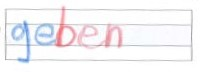
\includegraphics[]{figures/Schreibliniensystem.jpg}
    \caption{Schreibliniensystem mit Oberband (Bereich zwischen der oberen und der zweiten Linie von oben), Mittelband (zwischen den beiden mittleren Linien) und Unterband.}
    \label{Schreibliniensystem}
\end{figure}

\is{Ober- und Unterlängen}Ober- und Unterlängen sind die Teile eines Buchstaben, die über das sogenannte Mittelband hinausragen. Abbildung~\ref{Schreibliniensystem} zeigt die Schreibung \textit{geben} in einem Schreibliniensystem für Erstklässler. Der Bereich zwischen den beiden mittleren Linien ist das Mittelband. Das Feld darüber nennt man das Oberband, das darunter das Unterband. Oberlängen befinden sich im Oberband, Unterlängen im Unterband. <g> hat also eine Unterlänge, <b> eine Oberlänge \citep[192--193]{FuhrhopPeters2013}. 

Silbengrenzen erkennt man im Geschriebenen  an den Ober- und Unterlängen \citep[217--221]{FuhrhopPeters2013}. Die Buchstabenform übernimmt in der geschriebenen Sprache also die Funktion, die die Sonorität der Laute (vgl. Abschnitt~\ref{subsec:Sonoritaet}), in der gesprochenen Sprache hat. Phonologisch gesehen beginnt das Wort \textit{geben} wenig sonor mit einem Plosiv. Die geringe Sonorität wird durch die Unterlänge des Buchstaben \textit{g} angezeigt. Bis zum Vokal \textipa{[e:]} steigt die Sonorität an. In der Schrift kann man das daran erkennen, dass das \textit{e} keine Ober- oder Unterlänge hat. Dann sinkt die Sonorität wieder ab bis zum \textipa{[b]}. Die Silbengrenze liegt also vor dem \textit{b}, dem Buchstaben mit der Oberlänge. Die hohe Sonorität des nächsten Sonoritätsgipfels kann man in der Schrift daran erkennen, dass \textit{e} keine Ober- oder Unterlänge hat. \textipa{[n]} ist ein sonorer Konsonant, der Buchstabe \textit{n} hat deshalb ebenfalls keine Ober- oder Unterlänge.

Allgemein kann man sagen, dass wenig sonore Laute meist Buchstaben mit Ober- oder Unterlängen entsprechen: \textit{p, b, t, d, k, g, h}. Die hochsonoren Vokale entsprechen Buchstaben ohne Ober- und Unterlängen: \textit{a, e, i, o, u}. 

Ober- und Unterlängen haben, wie \citet{Drews2011} zeigt, einen messbaren Einfluss auf die Lesegeschwindigkeit und Lesegenauigkeit. Das liegt daran, dass geübte Leserinnen und Leser nicht Buchstabe für Buchstabe lesen, sondern größere Einheiten auf einmal erfassen (\zB \cite{Scheerer-Neumann1998}). Über die Bereiche, die sie nicht genau lesen, stellen die Leserinnen und Leser Hypothesen an. Dabei helfen ihnen die Ober- und Unterlängen. Wenn sie anhand dieser beispielsweise wissen, dass ein Wort drei Silben hat, können sie eine deutlich präzisere Voraussage machen, um welches Wort es sich handeln könnte als wenn sie keine Information über die Anzahl der Silben haben.

Der Zusammenhang zwischen geringer Sonorität und den Ober- oder Unterlängen ist nicht absolut. Eine Ausnahme ist \textit{s}, ein Buchstabe, der meistens an Silbengrenzen steht, aber keine Ober- oder Unterlänge hat. Interessant ist in diesem Zusammenhang jedoch die Entwicklung, die das Deutsche in den letzten Jahrhunderten erlebt hat. Für das stimmlose \textipa{[s]} hat sich das \textit{ß}, ein Buchstabe mit Oberlänge, entwickelt \citep[199--200]{FuhrhopPeters2013}. Das Schreibsystem hat sich also in gewisser Weise repariert.

Als zweites Beispiel für die Entwicklung zu einer besseren Markierung von Silbengrenzen hin wird das \textit{y} betrachtet. Als Buchstabe mit Unterlänge ist es nicht gut geeignet, um einen vokalischen Silbenkern zu repräsentieren. Während das \textit{y} im Frühneuhochdeutschen aber noch sehr häufig war, wird es seitdem immer weiter verdrängt und durch <i> ersetzt, einen Buchstaben, welcher ohne Ober- und Unterlänge ein besserer graphematischer Silbenkern ist \citep[220--221]{FuhrhopPeters2013}.



\section{Buchstaben und Grapheme}\label{sec:BuchstabenGrapheme}

\is{syllabische Schrift}\is{Alphabetschrift}\is{logographische Schrift} Im Allgemeinen werden nach \citet[69--70]{Duerscheid2016} drei Schrifttypen unterschieden: der \textit{logographische} Schrifttyp, der \textit{syllabische} Schrifttyp und der \textit{alphabetischen} Schrifttyp. Bei Schriftsystemen vom logographischen Schrifttyp, zu denen etwa das Chinesische gehört, entspricht ein Schriftzeichen in der Regel einer bedeutungstragenden Einheit (\zB einem Wort oder einem Morphem). Bei Schriftsystemem vom syllabischen und alphabetischen Typ hingegen entsprechen die Schriftzeichen \textit{bedeutungsunterscheidenden Einheiten} (Silben beim syllabischen Typ, \zB Japanisch, und Lauten beim alphabetischen Typ, \zB Deutsch, Russisch, Griechisch).

Wenn ein Schriftzeichen in einer Alphabetschrift bedeutungsunterscheidend ist, bezeichnet man es als \textit{Graphem} \citep[202]{FuhrhopPeters2013}.

\begin{Definition}{Grapheme}\label{def:Grapheme}
    
\noindent Grapheme sind die kleinsten bedeutungsunterscheidenden Einheiten der Schriftsprache.
\end{Definition}



Ähnlich wie die Phoneme (Definition~\ref{def:Phonem}), gewinnt man die Grapheme eines Schriftsystems durch \textit{Minimalpaaranalyse}\is{Minimalpaar}. Dafür stellt man zwei Wörter, die sich in einem einzigen Schriftzeichen unterscheiden, gegenüber. Haben die beiden Wörter auch unterschiedliche Bedeutung, sind die beiden unterschiedlichen Schriftzeichen Grapheme. Wenn man beispielsweise \textit{als} und \textit{alt} vergleicht, stellt man fest, dass sie sich in einem Schriftzeichen unterscheiden, \textit{s} vs. \textit{t}. Außerdem gibt es einen Bedeutungsunterschied. Daraus kann man schlussfolgern, dass <s> und <t> Grapheme sind. Grapheme setzt man in spitze Klammern. 

\is{Graphem}Grapheme können aus genau einem Buchstaben bestehen, dann bezeichnet man sie als \textit{einfache Grapheme}\is{Graphem!einfach}, \zB <s, t, a, w>. Es gibt aber auch Grapheme, die aus mehreren Buchstaben bestehen (\textit{komplexe Grapheme})\is{Graphem!komplex}. Man kann etwa \textit{mich} und \textit{mit} kontrastieren und dadurch zeigen, dass <ch> und <t> Grapheme sind. <ch> ist ein komplexes Graphem, so wie auch <qu> und <sch>. Ein vokalisches komplexes Graphem ist <ie>.


Es ist wichtig, Buchstaben und Grapheme nicht gleichzusetzen. Es gibt
\begin{itemize}
    \item Buchstaben, die Grapheme des Deutschen sind, \zB <e>,
    \item Buchstaben, die keine Grapheme des Deutschen sind, \zB \textit{q},
    \item mehrere Buchstaben, die zusammen ein Graphem bilden \zB <ch>.
\end{itemize}


Das\is{Grapheminventar} im Folgenden aufgelistete Grapheminventar des Deutschen orientiert sich an der \citet[909f]{Duden2022}. Hinzugefügt sind lediglich die Schreibdiph\-thonge. Hier orientieren wir uns an \citet[210, 222]{FuhrhopPeters2013}, die bei der Auflistung der Graphem-Phonem-Korrespondenzen zwar keine Korrespondenzen zwischen lautlichen Diphthongen und Schreibdiphthongen angeben, später aber genau diese Korrespondenzen diskutieren. Die Annahme von Schreibdiphthongen als Grapheme kann man mit Minimalpaaren wie \textit{fielen - feilen, freuen - Frauen} begründen. Diese Grapheme anzunehmen ist außerdem sinnvoll für didaktische Implikationen.


\ea
\textit{Grapheminventar des Deutschen}\\
    \begin{itemize}
        \item einfache Grapheme: \textit{a, b, d, e, f, g, h, i, j, k, l, m, n, o, p, r, s, t, u, v, w, x, z, ß, ä, ö, ü}
        \item komplexe Grapheme: \textit{ch, qu, sch, ng, ie, ei, au, eu}
    \end{itemize}
\z



Einige der hier angegebenen Grapheme sind umstritten. Gegen das Graphem <ng> wird argumentiert, dass es zwei Lauten entspricht, von denen einer durch einen phonologischen Prozess getilgt wird (vgl. Abschnitt~\ref{sec:gTilgung}). \citet[94--97]{Nerius1989} bezeichnet <ng> als \gqq{Buchstabenverbindung}. \citet[209]{FuhrhopPeters2013} listen <ng> nicht als Phonem, führen es in Klammern allerdings bei den Phonem-Graphem-Beziehungen auf.  

Außerdem stellen \citet[205]{FuhrhopPeters2013} den Graphemstatus von <sch> infrage. Mittels der Minimalpaare \textit{Masche -- manche -- Maske}  zeigen sie, dass <s> und <ch> separat ersetzbar sind. Das Minimalpaar \textit{Masche -- manche} zeigt demnach, dass das <s> innerhalb des <sch> ein Graphem ist. Das Minimalpaar \textit{Masche -- Maske} zeigt, dass das <ch> innerhalb des <sch> ein Graphem ist. Gegen diese Analyse kann man einwenden, dass ein Graphem eine lautliche Einheit repräsentiert. Wenn man <sch> als zwei Grapheme betrachtet, müsste diesen beiden Graphemen eine Phonemfolge entsprechen, was aber nicht der Fall ist.

Bei <ie> wird diskutiert, dass die Gespanntheit im Deutschen in der Regel nicht am Graphem selbst angezeigt wird (\cite[211]{FuhrhopPeters2013}, \cite[24]{Primus2010}). 

Die Buchstaben \textit{c, y} und \textit{q} sind keine Grapheme des Deutschen, denn es gibt keine Minimalpaare, wo etwa \textit{c} mit einem anderen Graphem kontrastiert. \textit{c} kommt allein (also nicht als <ch> oder <sch>) nur in Fremdwörtern vor. \textit{y} kommt überhaupt nur in Fremdwörtern vor. \textit{q} kommt nur in der Verbindung <qu> vor: \textit{Qual, Quelle, quaken}.\footnote{Es gibt Minimalpaare, bei denen <qu> als Ganzes ersetzt wird: \textit{Qual -- Wal}. Dieses Minimalpaar zeigt, dass <qu> und <w> Grapheme des Deutschen sind. Man kann auch das \textit{q} alleine ersetzen: \textit{Quelle -- Duelle}.  Es gibt aber keine Möglichkeit das \textit{u} von <qu> zu ersetzen (etwa \textit{Quelle -- *Qielle}), cf. \citet[204]{FuhrhopPeters2013}.}

Die eher sprachdidaktisch orientierte Forschung tendiert dazu, <ng>, <sch>, <ie> und die Schreibdiph\-thonge als Grapheme zu behandeln, etwa \citet[21--22]{SchruenderLenzen2013}, die sich auf \citet{Thome2000a} bezieht.


\section{Phonem-Graphem-Korrespondenzen}\label{sec:PGK}

In Alphabetschriften gibt es regelhafte Entsprechungen zwischen Phonemen und Graphemen. Diese Entsprechungen nennt man \textit{Phonem-Graphem-Korres\-pon\-den\-zen}. Beispielsweise entspricht dem  Phonem \textipa{/l/} das Graphem <l>: \textit{leicht, Wal, Fohlen}. Bei den meisten Graphemen sind die Entsprechungen aber nicht 1:1. Beispielsweise kann ein \textipa{/p/} als <p> (\textit{Paar}), als <pp> (\textit{Klippe}) oder als <b> (\textit{hinab}) geschrieben werden. \citet[95--97]{Nerius1989} stellt die Beziehungen zwischen Phonemen und Graphemen daher konsistent als 1:x-Beziehungen dar. Wie weiter unten ausgeführt, folgt die sprachdidaktische Literatur bis heute diesem Ansatz. In der linguistischen Literatur hingegen, \zB in der \citet[910]{Duden2022}, wird jedem Phonem ein einziges Graphem zugeordnet, \zB dem \textipa{/p/} das <p>. Anders geartete Schreibungen, also <pp> oder <b> werden durch die weiteren graphematischen Prinzipien erklärt.

In den Tabellen~\ref{tab:PGBKonsonanten} und \ref{tab:PGBVokale} sind die Korrespondenzen in Anlehnung and die \citet[910--911]{Duden2022} dargestellt. Die IPA-Symbole entsprechen dabei denen, die in Kapitel~\ref{kap:Phonologie} eingeführt wurden. Nicht in der Duden-Grammatik aufgeführt sind die Korrespondenzen zwischen der Phonemfolge \textipa{/kv/} und <qu> und zwischen \textipa{/\t{ts}/} und <z>, die wir aber aufnehmen, weil wir <qu> und <z> als Graphem annehmen. Die \citet[911]{Duden2022} listet außerdem eine Korrespondenz zwischen \textipa{/\ae/} und <ä> auf. Wir folgen hier der phonetischen Literatur, die für das Deutsche nicht den Laut \textipa{[\ae]}, sondern das \textipa{[E]} vorsieht.


Während es bei den Konsonanten eine 1:1-Beziehung gibt -- jedem Phonem entspricht ein Graphem und umgekehrt (Tabelle~\ref{tab:PGBKonsonanten}) -- ist das bei den Vokalen nicht der Fall. Meist werden zwei Phoneme, ein ungespannter und ein gespannter Vokal, durch ein Graphem repräsentiert. Es existiert also eine 2:1- bzw. für <e> sogar eine 3:1-Beziehung. 1:1-Beziehungen gibt es nur bei \textipa{/i/} -- <ie> und \textipa{/I/} -- <i> (Tabelle~\ref{tab:PGBVokale}).

\begin{table}
    \centering
        \caption{\label{tab:PGBKonsonanten} Phonem-Graphem-Beziehungen für die Konsonanten}
    \begin{tabular}{llll}\lsptoprule
         Phoneme & Grapheme & Phoneme & Grapheme\\\midrule
         \textipa{/p/}&<p> & \textipa{/x/}&<ch>\\
         \textipa{/t/}&<t> & \textipa{/v/}&<w>\\
         \textipa{/k/}&<k> & \textipa{/z/}&<s>\\
         \textipa{/kv/}&<qu> & \textipa{/j/}&<j>\\
         \textipa{/b/}&<b> & \textipa{/h/}&<h>\\
        \textipa{/d/}&<d> & \textipa{/m/}&<m>\\
         \textipa{/g/}&<g> & \textipa{/n/}&<n>\\
         \textipa{/f/}&<f> & \textipa{/N/}&<ng>\\ 
         \textipa{/s/}&<ß> & \textipa{/l/}&<l>\\
         \textipa{/S/}&<sch> & \textipa{/K/}&<r>\\ 
         \textipa{/\t{ts}/}&<z> &\\\lspbottomrule
    \end{tabular}
\end{table}



\begin{table}
    \centering
    \begin{tabular}{llllll}\lsptoprule
         \multicolumn{2}{c}{gespannte Vokale}& \multicolumn{2}{c}{ungespannte Vokale}& \multicolumn{2}{c}{Diphthonge}\\
         Phoneme & Grapheme & Phoneme & Grapheme& Phoneme & Grapheme\\\midrule
         \textipa{/i/}&<ie> & \textipa{/I/}&<i>& \textipa{/\t*{aU}/}& <au>\\
         \textipa{/y/}&<ü> & \textipa{/Y/}&<ü>& \textipa{/\t*{OI}/}&<eu>\\
        \textipa{/e/}&<e> &\textipa{/E/}&<e>&\textipa{/\t*{aI}/}& <ei>\\
         \textipa{/\o/}&<ö> &\textipa{/\oe/}&<ö>\\
         \textipa{/a/}&<a> & \textipa{/a/}&<a>\\
         \textipa{/o/}&<o>& \textipa{/O/}&<o>\\
         \textipa{/u/}&<u> & \textipa{/U/}&<u>\\
          \textipa{/E/}&<ä> &\textipa{/@/}&<e>&\\ 
\lspbottomrule
    \end{tabular}
    \caption{\label{tab:PGBVokale} Phonem-Graphem-Beziehungen für die Vokale}
\end{table}

In der sprachdidaktischen Literatur geht man von 1:x-Beziehungen aus. \citet[84--93]{Thome2019} beispielsweise unterscheidet zwischen  \textit{Basisgraphemen} und \textit{Orthographemen}. Ein Phonem entspricht einem Basisgraphem und eventuell einem oder mehreren Orthographemen. Die Tabellen~\ref{BasisgraphemeOrthographeme1}  und \ref{BasisgraphemeOrthographeme2}  sind aus \citet{Thome2019} übernommen.

\begin{table}
    \centering
    \footnotesize
    \begin{tabular}{llllll}\lsptoprule
         Pho-&Basisgrapheme& \multicolumn{4}{c}{Orthographeme}\\
         eme&meist oder immer & manchmal & gelegentlich & selten & sehr selten\\\midrule
         \textipa{/n/}&<n> Nase & --&--&<nn> Tanne&--\\\hline
         \textipa{/r/}&<r> Rad &- &--&--&<rr> wirr\\
         &&&&&<rh> Rhein\\\hline
        \textipa{/t/}&<t> Tisch &-&<d> Bild&<tt> Mitte&<dt> Stadt\\
        &&&&&<th> Thron\\\hline
         \textipa{/d/}&<d> Dach&--&--&--&<dd> Kladde\\\hline
         \textipa{/l/}&<l> Lampe &--&<ll> Ball&--&--\\\hline
         \textipa{/s/}&<s> Eis& &<ss> Kuss&<ß> Gruß&-\\\hline
         \textipa{/x/}&<ch> Bach&--&--&<g> König&\\\hline
         \textipa{/m/}&<m> Maus&-- &<mm> Kamm&--&--\\\hline
         \textipa{/z/}&<s> Seil& --&--&--&--\\\hline
         \textipa{/f/}&<f> Fisch&<v> Vogel &--&<ff> Schiff&<ph> Physik\\\hline
         \textipa{/v/}&<w> Wiese& --&--&--&<v> Vase\\\hline
         \textipa{/g/}&<g> Gabel& --&--&--&<gg> Egge\\\hline
         \textipa{/k/}&<k> Kuchen&<g> Berg &<ck> Ecke&-&<ch> Chor\\
         &&&&&<c> Clown\\\hline
         \textipa{/b/}&<b> Buch& --&--&--&<bb> Ebbe\\\hline
         \textipa{/S/}&<sch> Schaf& <s> Spiel&-&-&-\\\hline
         \textipa{/h/}&<h> Haus& --&--&-&--\\\hline
         \textipa{/\t{ts}/}&<z> Zaun& -&<tz> Katze&--&--\\\hline
         \textipa{/p/}&<p> Pinsel& <b> Laub&--&<pp> Treppe&--\\\hline
         \textipa{/N/}&<ng> Ring& --&<n> Bank&--&--\\\hline
         \textipa{/j/}&<j> Junge& --&--&--&--\\\hline
         \textipa{/\t{pf}/}&<pf> Pferde Seil& --&--&--&--\\\hline
         \textipa{/\t{ks}/}&<chs> Fuchs& <x> Hexe&--&--&--\\
\lspbottomrule
    \end{tabular}
    \caption{\label{BasisgraphemeOrthographeme1}Basis- und Orthographeme der Konsonanten, übernommen aus: \citet[89]{Thome2019}}
\end{table}


\begin{table}
    \centering
    \footnotesize
    \begin{tabular}{llllll}\lsptoprule
         Pho-&Basisgrapheme& \multicolumn{4}{c}{Orthographeme}\\
         neme&meist oder immer & manchmal & gelegentlich & selten & sehr selten\\\midrule
         \textipa{/@/} & <e> Hase&-- &-- &-- &--\\\hline
         \textipa{/I/} & <i> Insel&-- &-- &-- &<ie> vierzig\\\hline
         \textipa{/a/} & <a> Apfel&-- &-- &-- &--\\\hline
         \textipa{/i:/} & <ie> Biene&-- &<ih> ihr &<i> Igel &<ieh> sieht\\\hline
         \textipa{/e:/} & <e> Feder&-- &<eh> sehr &-- &<ee> See\\\hline
         \textipa{/a:/} &<a> Glas &-- &-- &<ah> sah &<aa> Haar\\\hline
         \textipa{/E/} & <e> Zelt&-- &<ä> hält &-- &--\\\hline
         \textipa{/\t*{aI}/} & <ei> Ei &-- &-- &-- &<eih> Geweih\\
         &&&&&<ai> Mais\\\hline
         \textipa{/U/} & <u> Muschel&-- &-- &-- &--\\\hline
         \textipa{/O/} & <o> Frosch&-- &-- &-- &--\\\hline
         \textipa{/o:/} & <o> Hose&-- &<oh> Sohn &-- &<oo> Boot\\\hline
         \textipa{/u:/} & <u> Blume&-- &-- &<uh> Kuh &--\\\hline
         \textipa{/\t*{aU}/} & <au> Auto &-- &-- &-- &--\\\hline
         \textipa{/y:/} &  <ü> Hüte&<üh> Kühe &-- &-- &--\\\hline
         \textipa{/Y/} & <ü> Büsche&-- &-- &-- &--\\\hline
         \textipa{/\o:/} &<ö> Löwe &-- &<öh> Söhne &-- &--\\\hline
         \textipa{/\t*{OY}/} & <eu> Eule&&<äu> läuten  &-- &--\\\hline
         \textipa{/E:/} &<ä> Käse &<äh> Fähre &-- &-- &--\\\hline
         \textipa{/\oe /} &<ö> Töpfe &-- &-- &-- &--\\
         \lspbottomrule
    \end{tabular}
    \caption{\label{BasisgraphemeOrthographeme2}Basis- und Orthographeme der Vokale, übernommen aus: \citet[89]{Thome2019}}
\end{table}
         

\is{Basisgraphem}Basisgrapheme sind Grapheme, die häufig vorkommen. \is{Orthographem}Orthographeme sind Grapheme, die selten vorkommen. Thomé geht davon aus, dass der Erwerb der Basisgrapheme dem der Orthographeme vorangeht. Zum Beispiel wird <p> als Basisgraphem für das Phonem \textipa{/p/} zuerst erworben; <b> oder <pp> sind Orthographeme für \textipa{/p/} und werden daher später erworben \citep[89--90]{Thome2019}. 

Die Korrespondenzen bei den s-Lauten unterscheiden sich ebenfalls. Während die \citet[910]{Duden2022} von einer 1:1-Zuordnung ausgeht: \textipa{/s/} -- <ß> und \textipa{/z/} -- <s>, nimmt \citet{Thome2019} <s> als Basisgraphem für beide Laute, \textipa{/s/} und \textipa{/z/} an, weil der Laut \textipa{[s]} durch die Auslautverhärtung häufig <s> geschrieben wird.

Genau wie die Duden-Grammatik geht Thomé bei den Vokalgraphemen von einer grundsätzlichen 2:1-Beziehung zwischen Phonemen und Basisgraphemen aus. So entspricht dem Basisgraphem <u> das Phonem \textipa{/u:/} (\textit{Blume}), aber auch das Phonem \textipa{/U/} (\textit{Muschel}). Bei <e> gibt es -- wie in der \citet{Duden2022} -- eine 1:3-Beziehung. Diesem Graphem entsprechen die Phoneme \textipa{/@, e, E/}, etwa in den Wörtern \textit{Hase, Feder, Zelt}. Bei den i-Lauten nimmt Thomé -- wie die Duden-Grammatik -- eine 1:1-Beziehung an: <ie> entspricht \textipa{/i:/} und <i> entspricht \textipa{/I/}.\footnote{Die Unterscheidung zwischen Basisgraphemen und Orthographemen ist insofern nützlich, als man im Erwerb tatsächlich beobachten kann, dass zunächst die Basisgrapheme und erst danach die Orthographeme erworben werden. Strenggenommen sind jedoch die Orthographeme häufig keine Grapheme, denn Grapheme sind die \textit{kleinsten} bedeutungsunterscheidenden Einheiten der Schriftsprache. \citet[89]{Thome2019} listet beispielsweise für \textipa{/a:/} als Basisgraphem <a> wie in \textit{Glas} und als Orthographem <ah> wie in \textit{sah} auf. Da man sowohl das <h> als auch das <a> ersetzen kann, um ein Minimalpaar zu bilden (\textit{Sau} und \textit{sieh}), handelt es sich bei <ah> nicht um die kleinste bedeutungsunterscheidende Einheit. Diesen Einwand kann man -- wie bei \citet{FuhrhopThierrof2005} dargestellt -- zwar auch beim <sch> bringen. Bei <sch> kann man jedoch argumentieren, dass <s> und <ch> anderen Lauten entsprechen als <sch>. Ein weiterer Einwand gegen den Phonembegriff bei Thomé ist, dass <chs> zwar eine häufige Schreibung ist, das ihm zugeordnete \textipa{/ks/} jedoch kein Phonem, sondern eine Phonemfolge ist. Deshalb sind viele Autor(inn)en der Meinung, dass <chs> eigentlich zwei Grapheme sind, <ch> und <s>, \zB \citet[96]{Nerius1989}, der bei \textit{Wachs} eine Entsprechung <ch> -- \textipa{/k/} und eine weitere <s> -- \textipa{/s/} annimmt.}

\largerpage
Ein Vorteil von Thomés Ansatz ist, dass er Erwerbsreihenfolgen gut erklärt. Beispielsweise wird \textipa{/s/} durch die Auslautverhärtung tatsächlich häufig <s> geschrieben und diese Zuordnung wird auch früher erworben als die \textipa{/s/} -- <ß>-Zuordnung.

\largerpage
Ein Nachteil des Ansatzes von Thomé ist, dass die Annahme von Orthographemen wenig erklärt und damit die Chance vertan wird, Regelhaftes in der Orthografie als solches zu erkennen. Auch das kann man an der Analyse der s-Laute zeigen. Thomé erklärt mit der Zuordnung von \textipa{/s/} und \textipa{/z/} zu <s> nur, dass die meisten Wörter, in denen \textipa{[s]} gesprochen wird, mit <s> geschrieben werden. Das stimmt, es hilft aber nicht, wenn man sich fragt, ob man \textit{Gras} oder \textit{*Graß} schreiben muss. Hier wird Regelhaftes als arbiträr dargestellt: Bei \textit{Gras} und \textit{Eis} handelt es sich um Schreibungen, die morphologisch (also über Ableitungen) zu begründen sind. Man schreibt \textit{Gras}, weil es \textit{Gräser} (mit \textipa{[z]}) gibt und \textit{Eis}, weil es \textit{eisig} (mit \textipa{[z]}) gibt.

\newpage
Auch die Schreibung der Doppelkonsonanz wird als etwas Arbiträres dargestellt. Nach Thomés Ansatz müsste man die Schreibung \textit{Mitte} mit zwei unabhängigen Überlegungen begründen: (1) <i> ist das Basisgraphem von \textipa{/I/}, (2) <tt> ist ein Orthographem von \textipa{/t/}. Dass beides miteinander zusammenhängt, dass man die Aussprache \textipa{/I/} also aus der Schreibung <tt> ableiten kann, wird durch diese Analyse nicht klar.

Linguistisch gesehen ist es also wenig sinnvoll, Orthographeme überhaupt als Grapheme anzusehen. Davon abgesehen werden durch sie regelhafte Schreibungen als arbiträr dargestellt. Deshalb werden wir im Folgenden als Phonem-Graphem-Korrespondenzen die Korrespondenzen aus der \citet[]{Duden2022} betrachten, die meist den Korrespondenzen zwischen Phonemen und Basisgraphemen bei Thomé entsprechen. Die Schreibungen, die Thomé als Orthographeme bezeichnet, werden wir über die weiteren Prinzipien der Orthografie erklären.

\section{Graphematische Prinzipien}\label{sec:GraphPrin}\is{graphematische Prinzipien}
Die Schreibung des Deutschen ist durch bestimmte Grundsätze geprägt. Diese Grundsätze nennt man \textit{graphematische Prinzipien}. Der wichtigste Grundsatz jeder Alphabetschrift ist das \textit{phonographische Prinzip}. Nach diesem Prinzip wird jedem Phonem ein Graphem zugeordnet. Nach dem \textit{silbischen Prinzip} kennzeichnet man bei Schreibungen Eigenschaften, die mit der Silbenstruktur zu tun haben, beispielsweise ein Silbengelenk durch eine Doppelkonsonanz (\zB \textit{Fussel}). Nach dem \textit{morphologischen Prinzip} schreibt man verwandte Stämme gleich oder zumindest ähnlich (\zB \textit{Stämme} mit <ä>, weil der Singular \textit{Stamm} ist). Nach dem \textit{syntaktischen Prinzip} schreibt man so, dass man die syntaktische Struktur einer Äußerung erkennen kann. Die Großschreibung nominaler Köpfe (Substantive) ist eine Ausprägung des syntaktischen Prinzips. Einige Schreibungen lassen sich darüber erklären, dass man versucht, gleichlautende Wörter (etwa \textit{Leib -- Laib}) unterschiedlich zu schreiben. Diese Schreibungen lassen sich über das \textit{Homographievermeidungsprinzip} erklären. In der Literatur werden noch weitere Prinzipien diskutiert, etwa das ästhetische Prinzip oder das historische \citep[88--98]{Nerius2007} die wir hier aussparen wollen.

Die Reihenfolge, in welcher die Prinzipien diskutiert werden, ist nicht willkürlich. Das zuerst genannte Prinzip, das phonographische, ist zugleich das dominanteste. Das zuletzt genannte Homographievermeidungsprinzip hat deutlich weniger Einfluss. Wenn Prinzipien miteinander konkurrieren, \gqq{gewinnt} in der Regel das grundlegendere Prinzip. Die Erwerbsreihenfolge der ersten vier Prinzipien entspricht in etwa der hier angegebenen Reihenfolge, d.\,h. zunächst schreiben Lernende nach dem phonographischen Prinzip, später kommen silbische Schreibungen dazu, noch später morphologische. Schreibungen nach dem syntaktischen Prinzip werden manchmal erst gegen Ende der Schulzeit perfektioniert (vgl. Abschnitt~\ref{sec:Erwerbsreihenfolgen}). 


\subsection{Phonographisches Prinzip}
\label{Absatz_phon_prin}


Das \textit{phonographische Prinzip} (auch \textit{phonologisches} oder \textit{phonematisches Prinzip, Lautprinzip}) lässt sich vereinfacht wie folgt fassen:


\begin{Definition}{Phonographisches Prinzip}\\
\noindent Den lautlichen Elementen (Phonemen) sind in der Schriftsprache schriftliche Elemente (Grapheme) zugeordnet.\footnote{Für explizitere Formulierungen cf. etwa \citet[144]{Duerscheid2016}, \citet[40]{GallmannSitta1996}.}
\end{Definition}

Im Folgenden werden vier Wörter betrachtet: \textit{mit, mich, bitte} und \textit{Kiel}. Das Wort \textit{mit} besteht im Standard aus drei Phonemen: \textipa{/mIt/}. Um die \textit{phonographische Schreibung} zu ermitteln, wird jedes Phonem durch das Graphem ersetzt, welches ihm laut Graphem-Phonem-Korrespondenzen entspricht (Tabellen~\ref{tab:PGBKonsonanten},  Seite \pageref{tab:PGBKonsonanten}, und \ref{tab:PGBVokale}, Seite \pageref{tab:PGBVokale}): 

\ea
\begin{tabular}{lccc}
Phoneme: & \textipa{/m/} & \textipa{/I/} & \textipa{/t/}\\
&| & | & |\\
Grapheme: & <m> & <i> & <t>\\
\end{tabular}
\z

Die Schreibung <mit> wird als phonographische Schreibung bezeichnet, denn sie ergibt sich allein aufgrund der Graphem-Phonem-Korrespondenzen.

Das Wort \textit{mich} besteht ebenfalls aus drei Phonemen: \textipa{/mIç/}. Nun wird wieder jedes der Phoneme durch das entsprechende Graphem ersetzt: \textipa{/m/} durch <m>, \textipa{/I/} durch <i> und \textipa{/ç/} durch das komplexe Graphem <ch>:

\ea \begin{tabular}{lccc}
Phoneme: & \textipa{/m/} & \textipa{/I/} & \textipa{/ç/}\\
&| & | & |\\
Grapheme: & <m> & <i> & <ch>\\
\end{tabular}
\z


Es ergibt sich die Schreibung <mich>. Auch diese Schreibung ist also phonographisch.

Das Wort \textit{bitte} besteht aus vier Phonemen: \textipa{/\textprimstress bI\.*{t}@/}. Man ersetzt wieder jedes dieser Phoneme durch ein Graphem:

\ea
\begin{tabular}{lcccc}
Phoneme: & \textipa{/b/} & \textipa{/I/} & \textipa{/t/} & \textipa{/@/}\\
&| & | & |&\\
Grapheme: & <b> & <i> & <t> & <e>\\
\end{tabular}
\z

Bei der Schreibung <bite> handelt es sich um eine \textit{phonographische} Schreibung, aber nicht um eine \textit{orthografische} Schreibung. Um zur orthografischen Schreibung zu gelangen, muss man weitere Prinzipien (in diesem Fall das silbische Prinzip) berücksichtigen.

\textit{Kiel} besteht aus drei Phonemen: \textipa{/ki:l/}. 

\ea
\begin{tabular}{lccc}
Phoneme: & \textipa{/k/} & \textipa{/i:/} & \textipa{/l/}\\
&| & | & \\
Grapheme: & <k> & <ie> & <l>\\
\end{tabular}
\z

Wenn man von der Großschreibung absieht, ist \textit{Kiel} also eine phonographische Schreibung, denn dem gespannten \textipa{/i/} entspricht als Graphem <ie>.

Schreibungen von Kindern zu Beginn des Schriftspracherwerbs orientieren sich zunächst vor allem am phonographischen Prinzip. Der folgende Text wurde von einer Zweitklässlerin geschrieben (Alter: 7;11). 

\ea
\ea
    \textit{Nach ein pa Wochen bekam die Muter en Kind das nanten sie Wiki. Wiki wuks her ran und waso gros widianderin. alz er 9 Jare alt wa sagte die Muter past auf die Hae auf. wensie euch Fresen dan seit ir Tot...}
\ex
    In Standardorthografie: \textit{Nach ein paar Wochen bekam die Mutter ein Kind, das nannten sie Wiki. Wiki wuchs heran und war so groß wie die anderen. Als er 9 Jahre alt war, sagte die Mutter: Passt auf die Haie auf. Wenn sie euch fressen, dann seid ihr tot...}
\z
\z

Der Text enthält Wörter, deren Orthografie sich tatsächlich nur aus dem phonographischen Prinzip ableitet: \textit{nach, Wochen, bekam, die, das} usw. Darüber hinaus schreibt das Kind Wörter phonographisch, bei denen für die orthografische Schreibung weitere Prinzipien beachtet werden müssen: Bei \textit{Jare, Fresen} das silbische Prinzip und bei den meisten Wörtern mit \textipa{/K/}-Vokalisierung (\textit{pa, wa}) das morphologische Prinzip.

Wenn man von der Groß- und Kleinschreibung, die hier noch sehr willkürlich eingesetzt wird, absieht, dann gibt es in diesem Text lediglich drei Schreibungen, bei denen andere Prinzipien als das phonographische Prinzip beachtet wurden: \textit{Kind} (statt phonographisch \textit{kint}), \textit{und} (statt phonographisch \textit{unt}) und \textit{sagte} (statt phonographisch \textit{sakte}). Da es sich um häufige Wörter handelt, ist es möglich, dass das Kind die anderen Prinzipien nicht im eigentlichen Sinne \gqq{beachtet} hat, sondern die Wörter memoriert hat.

Wenn man von \textit{Phonem-Graphem-Beziehungen} spricht, könnte man auch die \textipa{/g/}-Schreibung bei \textit{Tag} oder \textit{lustig} als Schreibung nach den Graphem-Phonem-Korrespondenzen annehmen, weil Phoneme nämlich -- im Unterschied zu den Phonen -- Abstraktionen über die (tatsächlich produzierten) Phone sind. Phoneme sind also die Einheiten, die im mentalen Lexikon repräsentiert sind. Die phonologische Repräsentation von \textit{Tag} ist \textipa{/ta:g/}, die von \textit{lustig} ist \textipa{/\textprimstress lUs.tIg/}. Demzufolge wären \textit{Tag} und \textit{lustig} phonographische Schreibungen. Da man Phänomene des Schriftspracherwerbs auf diese Weise aber nicht erklären kann, weil der Zugriff auf die phonologische Repräsentation erst erlernt werden muss, werden wir der \citet[913f]{Duden2022} folgen und solche Schreibungen als morphologische Schreibungen analysieren.



\begin{Exkurs}{\gqq{Lesen durch Schreiben}, Anlauttabellen und Igel-Syndrom}
\label{ExkursIgelsyndrom}

\noindent In vielen Schulen wird der Erwerb der Phonem-Graphem-Korrespondenzen durch die Arbeit mit einer \textit{Anlauttabelle}\is{Anlauttabelle} gestützt. In einer solchen Tabelle ist jedem Graphem das Bild eines Gegenstandes oder Lebewesens zugeordnet, dessen Bezeichnung mit dem Laut beginnt, der durch das Graphem repräsentiert wird. Neben dem <k> ist etwa ein Koffer, neben dem <b> eine Banane. Die extremste Form der Arbeit mit der Anlauttabelle ist wohl der -- besonders in den Medien sehr umstrittene -- Ansatz nach Reichen \textit{Lesen durch Schreiben}\is{Lesen durch Schreiben} (\cite[]{Reichen2008} und \cite{WiemerHuettenberger2015}). Reichen zufolge sollte das Schreiben mit der Anlauttabelle dem Lesen vorangehen. Die Kinder sollen also zunächst versuchen, Wörter mittels der Tabelle zu verschriften. Das Lesen lernen sie, indem sie die von ihnen selbst verschrifteten Wörter versuchen zu lesen.

Die Anlauttabelle hat eine Art Siegeszug durch die Fibellandschaft absolviert. Kaum ein Lehrwerk für die Schuleingangsphase kommt heute mehr ohne Anlauttabelle aus, selbst wenn die Lehrwerke sonst methodisch relativ fern von Reichen verortet werden können.

\begin{figure}[!htbp]
\centering
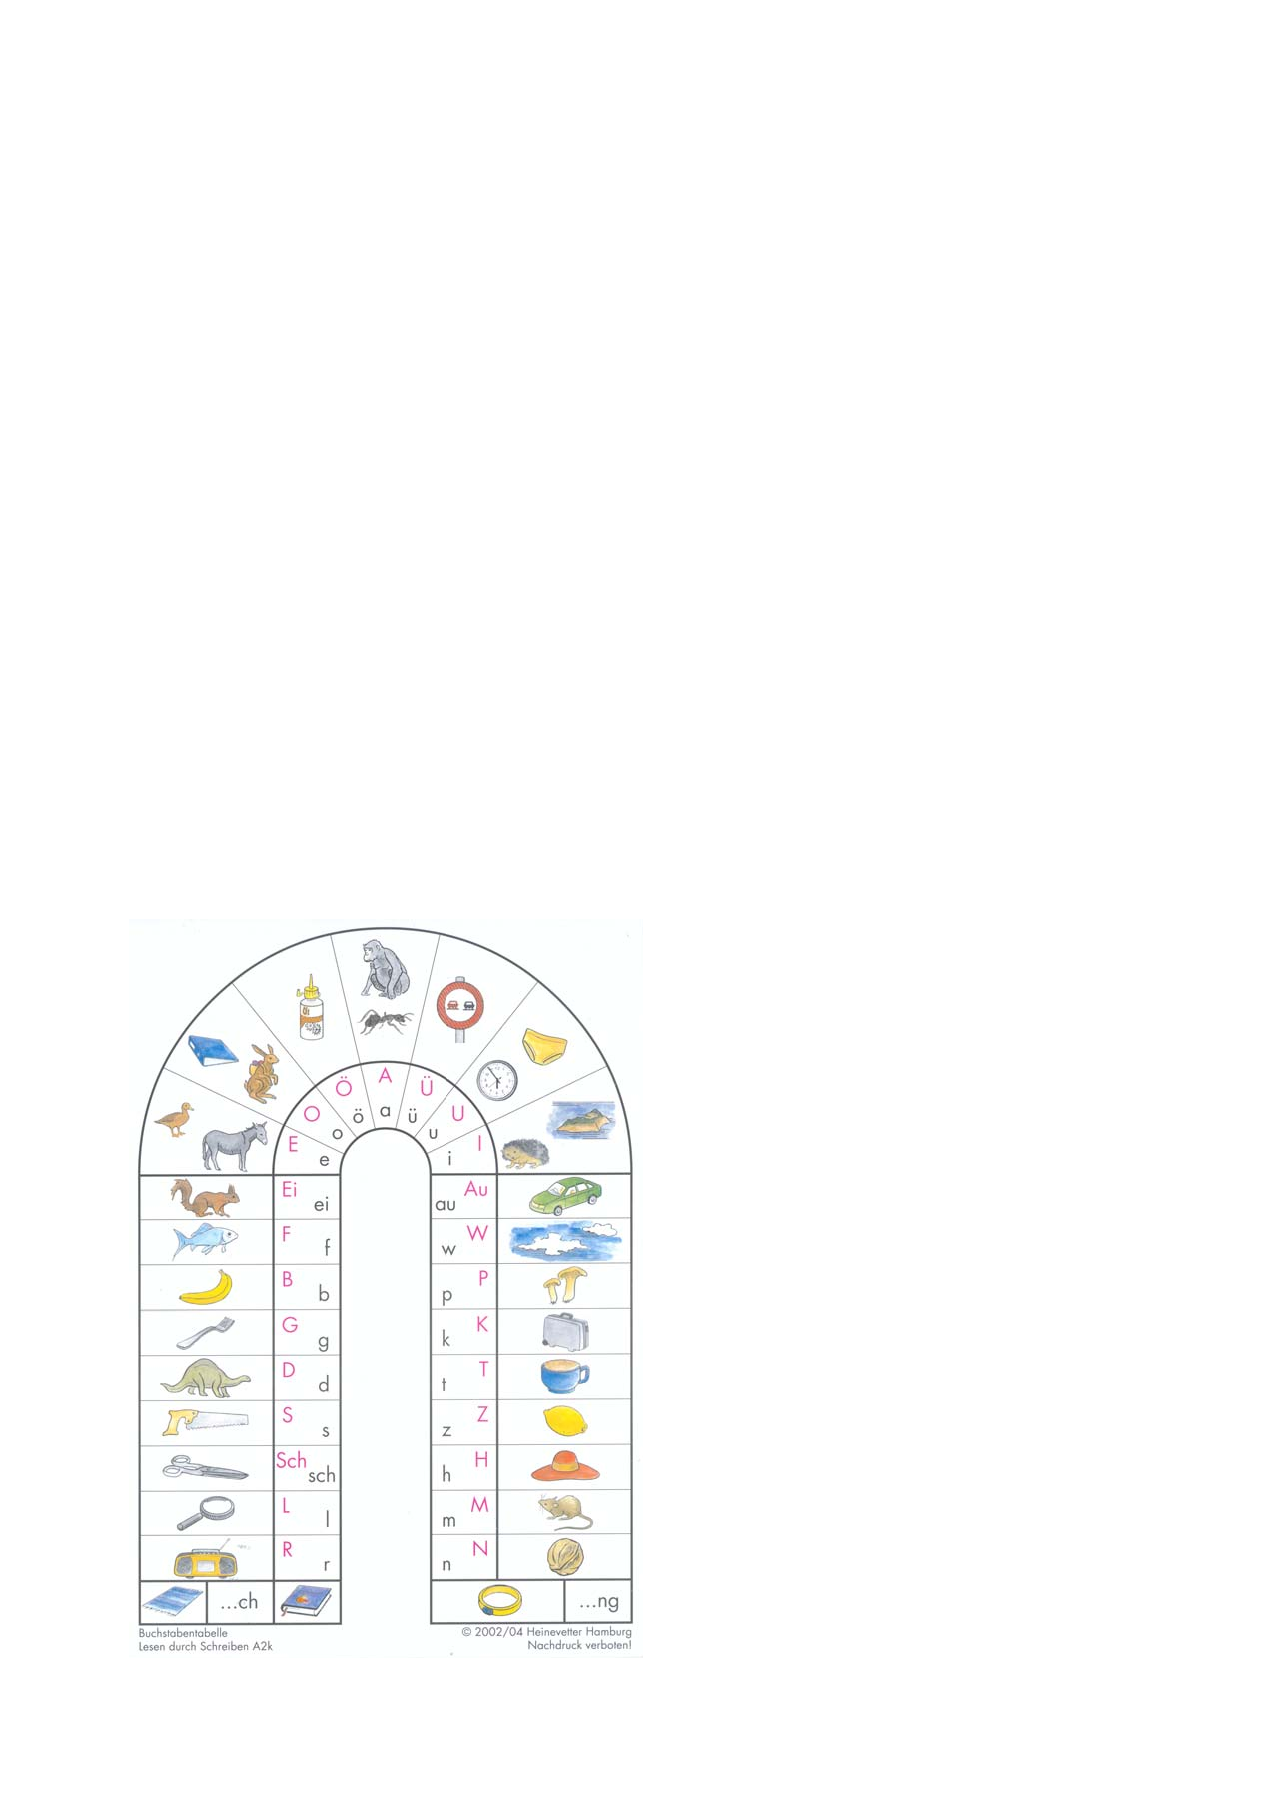
\includegraphics[width=.5\textwidth]{figures/Anlauttabelle_Reichen_2008.pdf}
\caption{Anlauttabelle aus \citet[4]{Reichen2008}}
\label{Anlauttabelle}
\end{figure}

Abbildung~\ref{Anlauttabelle} zeigt die Tabelle nach Reichen. Sie ist wie ein Tor geformt. In den Säulen stehen jeweils zwei Felder nebeneinander, im Bogen stehen sie übereinander. In dem einen der beiden Felder sind ein oder zwei Abbildungen zu sehen, in dem anderen ein Graphem (Großbuchstabe und Kleinbuchstabe). Die abgebildeten Lebewesen oder Gegenstände beginnen mit dem Laut, der über die Phonem-Graphem-Korrespondenzen dem jeweiligen Graphem zugeordnet ist. Der \textit{Dinosaurier} etwa beginnt mit dem Laut \textipa{/d/} und ist dem Graphem <D, d> zugeordnet. Die Konsonantengrapheme findet man in den beiden Säulen, die Vokalgrapheme im Bogen. Während man bei den Konsonantengraphemen eine 1:1-Relation findet (ein Bild pro Graphem), gibt es bei den Vokalgraphemen (außer bei <ü> und <ö>) zwei Bilder, die nur einem Graphem zugeordnet werden (\zB den \textit{Esel} für das gespannte \textipa{/e/} und die \textit{Ente} für das ungespannte \textipa{/E/}). 

Anlauttabellen sind im Prinzip Listen von Phonem-Graphem-Korres\-pon\-denzen für kindliche Nutzer. Reichen selbst hat unterschiedliche Anlauttabellen vorgeschlagen, \zB eine Erweiterung mit <eu, st, c, v, ä, pf, j, sp, x>. Die Tabellen der Schulbuchverlage heute unterscheiden sich zum Teil erheblich, vor allem in der Auswahl der bildlich dargestellten Beispielwörter. Für \textipa{/o/} beispielsweise wird \textit{Oma, Osterei} oder \textit{Ofen} angegeben, für \textipa{/l/} gibt es den \textit{Löwen} oder die \textit{Lupe}. Was jedoch immer gleich ist, ist die Korrespondenz zwischen \textipa{/i/} und dem \textit{Igel}. Wir werden gleich noch diskutieren, warum das so ist.

Warum ist die Methode nach Reichen so umstritten? Reichen selbst hat seine Methode nie wissenschaftlich evaluiert. Er beruft sich lediglich auf seine persönlichen Erfahrungen. Er argumentiert, dass die offene Unterrichtsform, die grundlegend für \textit{Lesen durch Schreiben} ist, die Motivation der Kinder hochhält, was sich positiv auf den Schriftspracherwerb auswirkt.

\citet{Weinhold2006} vergleicht in einer Longitudinalstudie den Schriftspracherwerb mittels der Reichen-Methode mit der silbenanalytischen Methode nach Röber (vgl. Exkurs~\ref{Exkurs:SAM}) und einem Fibellehrgang. Die Studie zeigt, dass die Reichen-Methode zumindest im ersten halben Schriftspracherwerbsjahr zu den besten Resultaten führt (S. 143). Die Anlauttabelle scheint für die Kinder in dieser Phase, wo sie sich vor allem am phonographischen Prinzip orientieren, also sehr nützlich zu sein. Danach überflügeln Klassen, die nach den anderen Methoden unterrichtet wurden, die Kinder, die nach der Reichen-Methode gelernt haben.

\citet{SchruenderLenzen2006} kann diesen anfänglichen Vorteil der Reichen-Methode in einer breit angelegten Studie nicht bestätigen. Die Kinder aus Klassen mit Fibellehrgängen erreichen am Ende der ersten Klasse bessere Werte (S. 34) im Rechtschreiben. Auch in der 3. Klasse sind die Fibelklassen den Klassen, die nach Reichen unterrichtet werden, überlegen (S. 35).

Neben der nicht nachgewiesenen Wirksamkeit\footnote{Nicht nachgewiesene Wirksamkeit ist ein Merkmal, welches diese Methode mit anderen teilt, cf. etwa \citet{BruegelmannBrinkmann2012}.} ist ein zweiter Grund dafür, dass die Methode umstritten ist, das sogenannte \textit{Igel-Syndrom}, cf. \citet[71]{Thome2019}\is{Igel-Syndrom}. Damit wird das Phänomen benannt, dass Kinder bis in die Mittelstufe hinein das gespannte \textipa{/i/} als <i> verschriften: <*Libe Oma!>; obwohl nach den Graphem-Phonem-Korrespondenzen <ie> geschrieben werden müsste. Bei <liebe> handelt es sich um eine phonographische Schreibung, also eine Schreibung nach dem phonographischen Prinzip. Obwohl phonographische Schreibungen generell früh erworben werden, sind ie-Fehlschreibungen häufig. \citet{Thome2000} argumentiert, dass das Igel-Syndrom eine direkte Folge der Arbeit mit der Anlauttabelle ist. In dieser Tabelle sind die Phonem-Graphem-Korrespondenzen für \textipa{/i, I/} schlicht falsch wiedergegeben. Für das ungespannte \textipa{/I/}, repräsentiert durch das Wort \textit{Insel}, wird richtigerweise <i> als Schreibung angegeben. Für das gespannte \textipa{/i/} wird mit <i> und dem \textit{Igel} jedoch eine falsche Korrespondenz angegeben.

Wenn die \textipa{/i/} -- <i>-Korrespondenz so selten vorkommt, warum verzichtet man dann nicht auf den \textit{Igel} und ersetzt ihn durch ein Wort mit der weitaus häufigeren Korrespondenz \textipa{/i/} -- <ie>? Das liegt daran, dass <ie> inital im Deutschen nicht vorkommt. Wörter, die mit \textipa{/i/} beginnen, werden mit <i> geschrieben: \textit{Igel, Iglu}. 

\citet[117]{Thome2000} schlägt deshalb statt einer Anlauttabelle eine Lauttabelle vor. Bei dieser Tabelle wird das Phonem \textipa{/i/} durch die \textit{Biene} repräsentiert. Damit wird die -- in der überwiegenden Mehrheit beobachtbare -- Graphem-Phonem-Korrespondenz \textipa{/i/} -- <ie> vermittelt. Es gibt inzwischen einige Lehrwerke, die das Problem angehen. Die Anlauttabelle der Tinto-Fibel etwa verzichtet zwar nicht auf den Igel, vermerkt aber zumindest die Möglichkeit der <ie>-Schreibung durch das Wort \textit{Knie} \citep[114]{Tintofibel}.
\end{Exkurs}

Zusammenfassend kann man feststellen, dass das phonographische Prinzip die Grundlage jeder Alphabetschrift ist. Jedem Phonem wird ein Graphem zugeordnet. Phonographische Schreibungen entstehen einzig und allein anhand dieser Zuordnung. Im Deutschen gibt es Wörter, die rein phonographisch geschrieben werden. Bei den meisten Schreibungen muss man jedoch weitere Prinzipien beachten.

\subsection{Silbisches Prinzip}\label{sec:silbischesPrinzip}
\is{silbisches Prinzip}

Die Beispiele im letzten Absatz haben gezeigt, dass phonographische Schreibungen nicht immer orthografisch sind. In den meisten Fällen greifen selbst bei der Schreibung einfacher Wörter mehrere Prinzipien. Viele betreffen die Silbe. Das liegt daran, dass -- wie eingangs erwähnt -- die Silbe für das Auge beim Lesen gut als Einheit erkennbar sein soll. Deshalb enthalten Schreibungen laut \citet[911ff]{Duden2022} auch silbenbezogene Informationen. 


Das silbische Prinzip hat vor allem zwei Ausprägungen: die \textit{Silbengelenksschreibung} (Konsonantenverdopplung oder \gqq{Schärfungsschreibung}\footnote{Der Begriff ist darauf zurückzuführen, dass die kurzen, ungespannten Vokale von einigen Sprecherinnen und Sprechern als scharf klingend empfunden werden.}) und die \textit{Dehnungsschreibung} (Doppelvokal oder \gqq{stummes h}).


\begin{Definition}{Silbisches Prinzip}

\noindent Schreibungen enthalten silbenbezogene Informationen, nämlich Informationen über die Vokallänge und das Vorhandensein eines Silbengelenks.


\end{Definition}



\subsubsection{Silbengelenksschreibungen}\label{sec:Silbengelenksschreibungen}
\is{Silbengelenksschreibung}


\subsubsubsection{Konsonantenverdopplung beim Silbengelenk}\is{Konsonantenverdopplung}
In Absatz~\ref{Absatz_phon_prin} wurde gezeigt, dass die Schreibung \textit{bitte} nicht allein über das phonographische Prinzip erklärt werden kann. Die phonographische Schreibung dieses Wortes ist <bite>. In der orthografischen Schreibung muss der Konsonant <t> verdoppelt werden.

In der didaktischen Literatur wird die Konsonantenverdopplung häufig \textit{Schärfungsschreibung}\is{Schärfungsschreibung} genannt. Zahlreiche erwachsene Schreiber(innen) formulieren die Regel für die Konsonantenverdopplung ähnlich wie in der folgenden Internetquelle\footnote{Richrath, Ulrike. 2020. Doppelkonsonanten: Zwei Regeln, die du dir leicht merken kannst. \url{https://die-lernlotsen.com/doppelkonsonanten-regeln} (28 Februar,
2020)}:

\begin{quote}
Hörst du den ersten Vokal im Wort kurz, dann schreibst du den nachfolgenden Mitlaut/ Konsonant [sic!] doppelt.[...] Hörst du den ersten Vokal im Wort lang, dann schreibst du den nachfolgenden Mitlaut nur einmal.
\end{quote}

Das stimmt für eine gewisse Anzahl an Wörtern: \textit{alle, Ratte, Fässer, Fälle, Hummel, Wippe, Fass, Fall} usw. Wenn man sich tatsächlich an diese Regel halten würde, würde man jedoch auch schreiben: \textit{*Felld, Hemmd, Hefft, Rosst, fünnf} usw. Die Regel scheint also falsch zu sein. Dass die Konsonantenverdopplung keine Folge der Aussprache des Vokals sein kann, zeigt auch der Vergleich zwischen Wörtern wie \textit{Sonne} und \textit{Sonde}. Die Vokale sind hier identisch und trotzdem wird der nachfolgende Konsonant einmal verdoppelt und das andere mal nicht. 

Andere Schreiberinnen und Schreiber des Deutschen geben an, sie würden die Doppelkonsonanten zweimal sprechen. Zu dieser Ansicht gelangen einige Sprecherinnen und Sprecher durch das Silbenklatschen von Wörtern mit Silbengelenk, bei denen der ambisilbische Konsonant doppelt gesprochen wird: \textit{al-le, Rat-te}. Auch zahlreiche Lehrmaterialien suggerieren, dass man ambisilbische Konsonanten doppelt spricht. Im \gqq{Rechtschreibführerschein} für die 2. Klasse \citep[AB 3.1.]{Dammeyer2010} steht dazu:

\begin{quote}
    Alle Mitlaute (Konsonanten), die in einem Wort \textit{zweimal} hintereinander \textit{gesprochen und geschrieben} werden, nennen wir Doppelmitlaute (Doppelkonsonanten).
\end{quote}

Wenn das der Fall wäre, wären Schreibungen wie \textit{alle, Fässer, Wippe} einfach phonographisch und sollten nach der Schuleingangsphase kein Problem mehr darstellen.

Einige Lehrkräfte und Lehrwerke vermitteln eine Regel, die deutlich mehr Fälle umfasst, etwa \citet[8]{MaierUsemann2015}:

\begin{quote}
Nach einem kurzen Vokal schreibst du fast immer mehrere Konsonanten: \textit{dunkel, schwanken}.
Wenn du dabei nur einen Konsonanten hörst, musst du ihn doppelt schreiben: \textit{rennen, Robbe}.
\end{quote}

Diese Regel erklärt alle bisher diskutierten Schreibungen, so auch die von \textit{Sonne} in Beispiel (\ref{ea:Sonne}) und \textit{Sonde} in Beispiel (\ref{ea:Sonde}):

\ea \label{ea:Sonne}
\begin{tabular}{cccc}
    [\textipa{z} & \textipa{O} & \textipa{\.*{n}} &\textipa{@}] \\
    | & | & |& |\\
    Konsonant & Vokal & Konsonant & Vokal\\
\end{tabular}
\z


Bei \textit{Sonne} folgt dem Kurzvokal \textipa{[O]} nur ein einziger gesprochener Konsonant: \textipa{[n]}. Diesen Konsonanten muss man in der Schreibung also verdoppeln: \textit{Sonne}.



\ea \label{ea:Sonde}
\begin{tabular}{ccccc}
    [\textipa{z} & \textipa{O} & \textipa{n} &\textipa{d}&\textipa{@}] \\
    | & | & |& | & |\\
    Konsonant & Vokal & Konsonant & Konsonant&Vokal\\
\end{tabular}
\z

Bei \textit{Sonde} ist das anders. Hier folgen dem Kurzvokal zwei Konsonanten, \textipa{[n]} und \textipa{[d]}. Man verdoppelt also nicht.

Warum hat sich in der Entwicklung der Schreibung eine solch kompliziert erscheinende Regel durchgesetzt? Wenn man die Wörter \textit{Sonne} und \textit{Sonde} phonologisch analysiert, ist die Regel eigentlich nicht kompliziert, vgl. Abbildung~\ref{fig:KonstSonne} und \ref{fig:KonstSonde}. Bei \textit{Sonne} ist das \textipa{/n/} ein Silbengelenk, bei \textit{Sonde} nicht. Als Silbengelenk wird das <n> verdoppelt, sodass jeder Buchstabe eindeutig einer Schreibsilbe zugeordnet werden kann. Die Schärfungsschreibung markiert also gar nicht den kurzen Vokal, sondern das Silbengelenk. Deshalb bezeichnet man die Konsonantenverdopplung auch als \textit{Silbengelenksschreibung}. Während der gesprochene Laut ambisilbisch\is{ambisilbischer Konsonant} ist, also zu beiden Silben gehört, sind die Schreibsilben getrennt: \textit{Son-ne}.


\begin{figure}
   \begin{forest}
   [Wort
       [σ, calign=last
         [Onset, ake
           [X
             [\textipa{z}]
           ]
         ]
         [Reim, calign=first
           [Nukleus, ake
             [X
           [\textipa{O}]
             ]
           ]
           [Koda, ake, name=ERBaum]
         ]
       ]
       [σ, calign=last
         [Onset, ake
           [X
             [\textipa{\.*{n}}]
           ]
           {\draw[-] (.north) -- (ERBaum.south);}
         ]
         [Reim
           [Nukleus, ake
           [X
             [\textipa{@}]
             ]
           ]
           [Koda, ake
           ]
         ]
       ]
      ]
   \end{forest}
   \caption{Konstituentenanalyse von \textit{Sonne}. Das \textipa{/n/} ist ein Silbengelenk.}
   \label{fig:KonstSonne}
\end{figure}

\begin{figure}
  \centering
  \begin{forest}
  [Wort
      [σ, calign=last
        [Onset, ake
          [X 
          [\textipa{z}]
          ]
        ]
        [Reim, calign=first
          [Nukleus, ake
            [X
            [\textipa{O}]
            ]
          ]
          [Koda, ake
          [X
          [\textipa{n}]
          ]
          ]
        ]
      ]
      [σ, calign=last
        [Onset, ake
          [X
          [\textipa{d}]
          ]
        ]
        [Reim, calign=first
          [Nukleus, ake
            [X
            [\textipa{@}]
            ]
          ]
          [Koda, ake
          ]
        ]
      ]
     ]
  \end{forest}
  \caption{Konstituentenanalyse von \textit{Sonde}. Das \textipa{/n/} gehört zur ersten Silbe.}
  \label{fig:KonstSonde}
\end{figure}


Wenn man noch einmal\is{Doppelkonsonanz} zu den zu Beginn des Abschnittes diskutierten Beispielen zurückkehrt, kann man feststellen, dass die meisten von ihnen ein Silbengelenk haben: \textit{alle, Ratte, Fässer, Fälle, Hummel, Wippe}. Die anderen beiden Wörter, \textit{Fass} und \textit{Fall}, sind Wörter, die mit einem Wort mit Silbengelenk verwandt sind, nämlich \textit{Fässer} bzw. \textit{fallen}. Bei diesen Wörtern liegt keine silbische Schreibung vor, sondern eine morphologische, vgl. Abschnitt~\ref{sec:MorphPrin}. Die Schärfungsschreibung verweist also immer auf ein Silbengelenk. Entweder befindet sich dieses im Wort selbst oder aber in einem verwandten Wort.

\subsubsubsection{Silbengelenksschreibung bei komplexen Graphemen}
\is{Graphem!komplex}
Die Wörter \textit{Tasse} und \textit{Tasche} wurden schon im Kapitel zur Phonologie analysiert, vgl. Abbildung~\ref{fig:KonstTasse} und \ref{fig:KonstTasche}. Sie werden hier erneut betrachtet.

\begin{figure}[!htbp]
  \centering
  \begin{forest}
  [Wort
      [σ, calign=last
        [Onset, ake
          [X
          [\textipa{t}]
          ]
        ]
        [Reim, calign=first
          [Nukleus, ake
            [X
            [\textipa{a}]
            ]
          ]
          [Koda, ake, name=ERBaum]
        ]
      ]
      [σ, calign=last
        [Onset, ake
          [X
          [\textipa{\.*{s}}]
          ]
          {\draw[-] (.north) -- (ERBaum.south);}
        ]
        [Reim
          [Nukleus, ake
            [X
            [\textipa{@}]
            ]
          ]
          [Koda, ake
          ]
        ]
      ]
     ]
  \end{forest}
  \caption{Konstituentenanalyse von \textit{Tasse}. \textipa{/s/} ist ein Silbengelenk.}
  \label{fig:KonstTasse}
\end{figure}

\begin{figure}[!htbp]
  \centering
  \begin{forest}
  [Wort
      [σ, calign=last
        [Onset, ake
          [X
          [\textipa{t}]
          ]
        ]
        [Reim, calign=first
          [Nukleus, ake
            [X
            [\textipa{a}]
            ]
          ]
          [Koda, ake, name=ERBaum]
        ]
      ]
      [σ, calign=last
        [Onset, ake
          [X
          [\textipa{\.*{S}}]
          ]
          {\draw[-] (.north) -- (ERBaum.south);}
        ]
        [Reim
          [Nukleus, ake
            [X
            [\textipa{@}]
            ]
          ]
          [Koda, ake
          ]
        ]
      ]
     ]
  \end{forest}
  \caption{Konstituentenanalyse von \textit{Tasche}. \textipa{/S/} ist ein Silbengelenk.}
  \label{fig:KonstTasche}
\end{figure}

Beide Wörter haben exakt dieselbe Silbenstruktur. Beide haben ein Silbengelenk. Die Schreibung unterscheidet sich jedoch: Bei \textit{Tasse} wird der Konsonant verdoppelt, bei \textit{Tasche} nicht. Die Beispiele in Tabelle~\ref{tab:SilbengelenkEinfKompl} zeigen die Regel hinter diesen Schreibungen: \is{Graphem!einfach}Einfache Grapheme werden als Silbengelenk verdoppelt, \is{Graphem!komplex}komplexe Grapheme jedoch nicht.


\begin{table}

    \caption{\label{tab:SilbengelenkEinfKompl} Silbengelenksmarkierung durch einfache und komplexe Grapheme}
\fittable{
\begin{tabular}{ll}
\lsptoprule
einfache Grapheme  (Verdopplung) &  komplexe Grapheme (keine Verdopplung)\\
     \midrule
     \textit{Tasse}& \textit{Tasche}  \\
     \textit{Massen}& \textit{machen}\\
     \textit{Wanne} & \textit{Wange}\\
     \lspbottomrule
\end{tabular}
}
\end{table}

Weil <s> und <n> einfache Grapheme sind, verdoppelt man bei den Beispielen \textit{Tasse, Massen} und \textit{Wanne}. Die Grapheme <sch>, <ch> und <ng> bestehen aus mehreren Buchstaben, sind also komplexe Grapheme. Man schreibt deshalb <Tasche, machen> und <Wange> und nicht <*Taschsche, *machchen> und <*Wangnge>. 

\subsubsubsection{Spezielle Silbengelenksschreibungen}\is{Silbengelenksschreibung!speziell}
\label{subsubsubsec:spezSG}
Zwei einfache Grapheme, die Grapheme <k> und <z>, haben eine sogenannte \textit{spezielle Silbengelenksschreibung}, nämlich <ck> und <tz>. Abbildung~\ref{fig:Konstanahacken} zeigt die Silbenstruktur eines Wortes mit <ck>, \textit{hacken}. \textipa{/k/} ist bei \textit{hacken} \textipa{[\textprimstress ha\.*k@n]} ein Silbengelenk. Man sollte nach der oben diskutierten Regel für die Silbengelenksschreibung also <hakken> schreiben. Aus historischen Gründen wird \textipa{/k/} als Silbengelenk jedoch <ck> geschrieben.\footnote{Das lateinische Alphabet verfügt über die Buchstaben <c> und <k>. In einigen älteren Sprachen repräsentierten diese beiden Grapheme zwei unterschiedliche Phoneme. Im Mittelhochdeutschen war das nicht mehr so, beide Buchstaben repräsentierten \textipa{/k/}. Unter diesen Umständen bekamen die beiden Buchstaben eine neue Funktion: Sie markierten Silbengrenzen. <k> wurde am Anfang einer Silbe verwendet, <c> am Ende \citep[156]{Paul2007}, etwa in mhd. \textit{danc} (nhd. \textit{Dank}), \textit{drec} (nhd. \textit{Dreck}), aber mhd. \textit{kal} für \textit{kahl}, \textit{keiser} für \textit{Kaiser} \citep{Grimm2020}. Ziel einer Silbengelenksschreibung ist es, zwei optisch trennbare Silben zu erzeugen, bei \textipa{['vEl@]} etwa \textit{Wel-le}. Da ein silbenfinales [k] <c> geschrieben wurde und ein silbeninitiales [k] <k>, ergab sich als Silbengelenksschreibung <ck>, etwa in \textit{Zuc-ker}.}\footnote{Anmerkung zur Silbentrennung am Zeilenende: Seit der letzten Orthografiereform wird nicht mehr \textit{hak-ken} getrennt, sondern \textit{ha-cken}.} Wenn die Affrikate \textipa{/\t{ts}/} ein Silbengelenk bildet, wird sie <tz> geschrieben. Ein Beispiel ist das Wort \textit{Mütze}, vgl. Abbildung~\ref{fig:KonstanaMuetze}. Wenn \textipa{/\t{ts}/} kein Silbengelenk ist, wird es einfach <z> geschrieben, \zB in \textit{Minze}.


\begin{figure}[!htbp]
  \centering
  \begin{forest}
  [Wort
      [σ, calign=last
        [Onset, ake
          [X
          [\textipa{h}]
          ]
        ]
        [Reim, calign=first
          [Nukleus, ake
            [X
            [\textipa{a}]
            ]
          ]
          [Koda, ake, name=ERBaum]
        ]
      ]
      [σ, calign=last
        [Onset, ake
          [X
          [\textipa{\.*{k}}]
          ]
          {\draw[-] (.north) -- (ERBaum.south);}
        ]
        [Reim
          [Nukleus, ake
          [X
          [\textipa{@}]
          ]
          ]
          [Koda, ake
            [X
            [\textipa{n}]
            ]
          ]
        ]
      ]
     ]
  \end{forest}
  \caption{Konstituentenanalyse von \textit{hacken}. \textipa{/k/} ist ein Silbengelenk, deshalb wird es orthografisch <ck> geschrieben.}
  \label{fig:Konstanahacken}
\end{figure}




\begin{figure}[!htbp]
  \centering
  \begin{forest}
  [Wort
      [σ, calign=last
        [Onset, ake
          [X
          [\textipa{m}]
          ]
        ]
        [Reim, calign=first
          [Nukleus, ake
          [X
            [\textipa{Y}]
          ]
          ]
          [Koda, ake, name=ERBaum]
        ]
      ]
      [σ, calign=last
        [Onset, ake
          [X
          [\textipa{\t{\.*{ts}}}]
          ]
          {\draw[-] (.north) -- (ERBaum.south);}
        ]
        [Reim
          [Nukleus, ake
          [X
          [\textipa{@}]
          ]
          ]
        ]
      ]
     ]
  \end{forest}
  \caption{Konstituentenanalyse von \textit{Mütze}. \textipa{/\t{ts}/} ist ein Silbengelenk. Orthografisch wird diese Affrikate als Silbengelenk durch <tz> repräsentiert.}
  \label{fig:KonstanaMuetze}
\end{figure}

\largerpage
Die speziellen Silbengelenksschreibungen\is{Silbengelenksschreibung!speziell} zeigen eindrücklich, dass Silbengelenksschreibungen ursächlich tatsächlich nichts mit der Kürze des Vokals zu tun haben. Die Wörter in Tabelle~\ref{tab:tzck} haben alle kurze Vokale, aber die Schreibung <tz> und <ck> findet man nur im Falle eines Silbengelenks.


Da die Silbengelenksschreibungen aber in den Schulen noch häufig mit Hinweis auf die Vokallänge unterrichtet werden, kommt es zu Schreibungen wie  \textit{*Höltzer, *Müntze, *Ancker}, es wird also <tz> statt <z> und <ck> statt <k> geschrieben.\footnote{Die Eselsbrücke \gqq{Nach l, n, r, das merke ja, steht nie tz und nie ck.} zielt genau auf diese Fälle ab: Wenn nach einem Vokal <l, n> oder <r> steht, kann es sich nicht um ein Silbengelenk handeln, denn ein Silbengelenk steht immer direkt nach einem Vokal.}\clearpage

\begin{table}
\caption{\label{tab:tzck} <tz> und <ck> als Silbengelenksschreibungen}
\begin{tabular}{lll}\lsptoprule
kein Silbengelenk & \textit{          }&Silbengelenk\\\midrule
     \textit{Hölzer} \textipa{[\textprimstress h\oe l.\t{ts}5]} &&  \textit{Klötzer} \textipa{[\textprimstress kl\oe \.*{\t{ts}}5]}\\
     \textit{Münze} \textipa{[\textprimstress mYn.\t{ts}@]}&&\textit{Mütze} \textipa{[\textprimstress mY\.*{\t{ts}}@]}\\
     \textit{Anker} \textipa{[\textprimstress PaN.k5]}&& \textit{hacken} \textipa{[\textprimstress ha\.*{k}@n]}\\
     \lspbottomrule
\end{tabular}
\end{table}



\begin{Exkurs}{Das Häusermodell nach Röber, Teil II}
\label{Exkurs:SAM}
\is{Häusermodell}

\noindent Die Ausführungen haben gezeigt, dass die Regel, die zahlreiche kompetente Schreiberinnen und Schreiber erinnern (\textit{Verdopple nach Kurzvokal!}), wenn man sie tatsächlich umsetzen würde, zu zahlreichen Fehlern führen würde, \zB <gellb> statt <gelb>. Gleichzeitig kann man aber beobachten, dass fortgeschrittene Schreiberinnen und Schreiber solche Fehler kaum machen. Die Regel \textit{Verdopple einen Konsonanten, der ein Silbengelenk darstellt!}, die deutlich mehr Fälle erfasst, wird offenbar implizit erworben. 

Es gibt einige Wissenschaftler(innen) und Lehrkräfte, die dafür argumentieren, dass die Schule sich nicht auf den impliziten Weg verlassen sollte, sondern den Erwerb der Schärfungsschreibung stärker steuern sollte, etwa Eichler (1976/1991) zitiert in \citet[72]{Bredeletal2017}. Eine Methode, dies zu tun, ist die Verwendung des \textit{Häusermodells} nach \citet{Roeber2013} , welches schon im Phonologiekapitel, Exkurs~\ref{ex:SAM_Grundlage}, Seite \pageref{ex:SAM_Grundlage}, eingeführt wurde. Röber stellt verschiedene Silbentypen graphisch unterschiedlich dar und leitet die Schreibung und die Lautung aus der Silbenstruktur ab. In Kapitel~\ref{kap:Phonologie} wurden die beiden Grundtypen von Häusern gezeigt. Diese beiden Typen werden hier noch einmal dargestellt, vgl. Abbildungen~\ref{fig:SAMHuete} und \ref{fig:SAMHuefte}.\is{Häusermodell} 

\begin{figure}
    \centering
    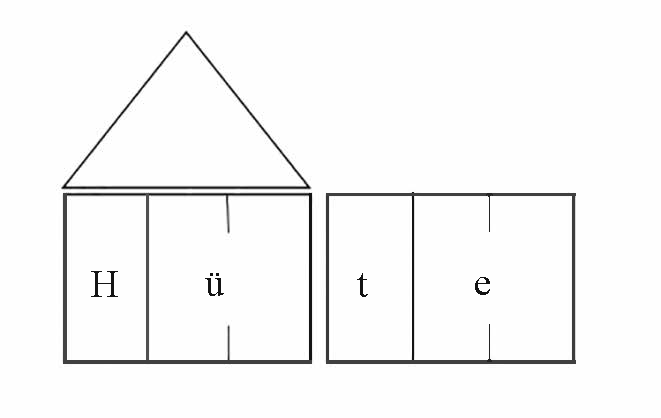
\includegraphics[width=0.5\textwidth]{figures/Huete.pdf}
    \caption{Darstellung der Silbenstruktur des Wortes \textit{Hüte} nach Röber. Die erste Silbe hat einen gespannten Vokal und ist offen.}
    \label{fig:SAMHuete}
\end{figure}

\begin{figure}
    \centering
    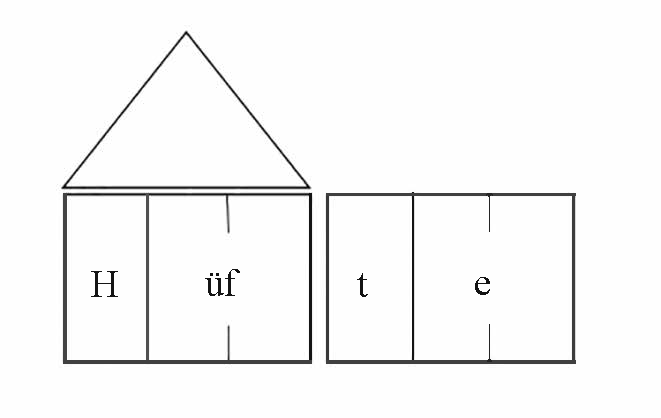
\includegraphics[width=0.5\textwidth]{figures/Huefte.pdf}
    \caption{Darstellung der Silbenstruktur des Wortes \textit{Hüfte} nach Röber. Die erste Silbe hat einen ungespannten Vokal und ist geschlossen.}
    \label{fig:SAMHuefte}
\end{figure}

Betonte Silben werden als Haus mit Dach dargestellt, unbetonte als Garage ohne Dach. Röber unterscheidet bei den betonten Silben zwei Silbentypen, die offene Silbe mit langem, gespannten Vokal (\textit{Hüte}-Typ, Abbildung~\ref{fig:SAMHuete}) und die geschlossene Silbe mit Kurzvokal (\textit{Hüfte}-Typ, Abbildung~\ref{fig:SAMHuefte}). 

Das Häusermodell kann die Unterscheidung zwischen gespannten und ungespannten Vokalen beim Lesen unterstützen und dadurch Leseaussprachen\is{Leseaussprache} wie \textipa{[\textprimstress hy:f.te:]} vermeiden helfen. Der Vokal im Haus mit Dach wird gespannt gesprochen, wenn er das große Zimmer im Haus allein bewohnt (\textit{Hüte}-Haus). Er wird ungespannt gesprochen, wenn er sich dieses Zimmer mit einem Konsonanten teilen muss (\textit{Hüfte}-Haus).\footnote{Man kann hier erkennen, warum das Modell mit Zweisilbern arbeitet. Diese Regularität gilt nämlich überhaupt nur für Zweisilber. Das Wort \textit{Hut} kann man nur unter Annahme einer weiteren Position für einen Konsonanten nach Langvokal analysieren, cf. \citet[166]{Roeber2013}.} Die Vokale der Garage werden reduziert gesprochen, meist entweder \textipa{[@]} oder \textipa{[5]}.

Für das Silbengelenk nimmt Röber einen weiteren Häusertyp an, den \textit{Hütte}-Typ. Bei diesem Häusertyp rutscht die Garage in das Haus mit Dach hinein, vgl. Abbildung~\ref{fig:SAMHuette}.

\begin{figure}
    \centering
    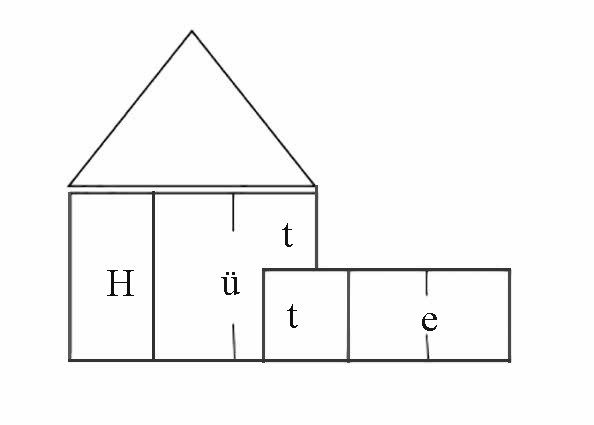
\includegraphics[width=0.5\textwidth]{figures/Huette.pdf}
    \caption{Darstellung der Silbenstruktur des Wortes \textit{Hütte} nach Röber}
    \label{fig:SAMHuette}
\end{figure}

Der Konsonant, der als Silbengelenk gesprochen wird, hat in diesem Häusertyp zwei Funktionen: Er muss als Mitbewohner im großen Zimmer zur Verfügung stehen, weil der Vokal sonst gespannt gesprochen werden würde. Außerdem muss er das erste Zimmer der zweiten Silbe besetzen. Diese Doppelfunktion wird in der Schreibung durch die Verdopplung des Konsonanten angezeigt.

Einzelne Aspekte dieses Modells haben Eingang in Lehrwerke gefunden, etwa in den Fibellehrgang \textit{ABC der Tiere} des Mildenberger-Verlags \citep[]{Handtetal2019}.

\end{Exkurs}

\subsubsection{Dehnungsschreibungen}
\label{AbschnittDehnungsh}
\is{Dehnungsschreibung}

Während die Konsonantenverdopplung -- wenn man sie als Signal für ein Silbengelenk interpretiert -- sehr systematisch ist, sind die Dehnungsschreibungen deutlich schwieriger über Regeln zu fassen. Im Deutschen existieren zwei Formen der Dehnungsmarkierung: das \textit{stumme h} und der \textit{Doppelvokal}. 

Schreibungen mit \is{Doppelvokal}Doppelvokal kommen etwa in folgenden Wörtern vor: \textit{Saat, Beet, Boot, Saal, Meer}. Einige dieser Schreibungen kann man dadurch begründen, dass Wörter von gleichlautenden anderen Wörtern unterschieden werden sollen, etwa \textit{mehr -- Meer}, vgl. auch Abschnitt~\ref{sec:Homographievermeidungsprinzip}. Abgesehen davon sind Doppelvokalschreibungen nur schwer durch Regeln zu fassen und müssen als \gqq{Merkwörter}\is{Merkwort} betrachtet werden. Doppelvokale stehen laut einer älteren Ausgabe der \citet[73--75]{Duden2016} vor allem bei einsilbigen Wörtern in offenen Silben, \zB in \textit{Fee, See}, sowie bei Zweisilbern, deren zweite Silbe mit <l, r, s> oder <t> beginnt: \textit{Meere, Aale}.

Im Gegensatz zu den recht unregelmäßigen Doppelvokalen\is{Doppelvokal} folgen die \textit{h}-Schreibungen\is{silbentrennendes h}\is{Dehnungs-h} einigen Gesetzmäßigkeiten, die im Folgenden diskutiert werden. Zunächst muss bei den h-Schreibungen zwischen dem sogenannten \textit{silbentrennenden h} (auch: silbeninitiales \textit{h}) und dem \textit{echten Dehnungs-\textit{h}} unterschieden werden. Das silbentrennende \textit{h} wird nämlich fast durchgängig geschrieben, während das Dehnungs-\textit{h} nur unter bestimmten Umständen geschrieben wird, die weiter unten genauer erläutert werden. 


Ein silbentrennendes \textit{h} trennt zwei vokalische Kerne. Es wird also immer dann gesetzt, wenn lautlich zwei Vokale aufeinandertreffen. Abbildung~\ref{Silbenstruktur_Muehe} zeigt die Silbenstruktur von \textit{Mühe}, Abbildung~\ref{Silbenstruktur_Muehle} die von \textit{Mühle}. Der wesentliche Unterschied liegt in der Besetzung des Onsets der zweiten Silbe.

\begin{figure}[!htbp]
  \centering
  \begin{forest}
  [Wort
      [σ, calign=last
        [Onset, ake
          [X
          [\textipa{m}]
          ]
        ]
      [Reim, calign=first
          [Nukleus, ake
            [X, name=X1 [,phantom ] 
                [\textipa{y:}, name=Y ]
            ]
            [X, name=X2 [,phantom ] 
            ]
          ]
        \draw (X1.south) -- (Y.north);
        \draw (X2.south) -- (Y.north);
          [Koda
      ]
      ]
      ]
      [σ, calign=last
      [\textcolor{darkgray}{Onset}
        ]
        [Reim
          [Nukleus, ake
            [X
            [\textipa{@}]
            ]
          ]
          [Koda
          ]
        ]
      ]
    ]
  \end{forest}
  \caption{Konstituentenanalyse von \textit{Mühe}: Der Onset der zweiten Silbe ist leer. Das geschriebene <h> ist also ein silbentrennendes h.}
  \label{Silbenstruktur_Muehe}
\end{figure}



Bei \textit{Mühe} sind die Koda der ersten Silbe und der Onset der zweiten Silbe leer. Dadurch treffen die beiden vokalischen Kerne direkt aufeinander. In der Schreibung dient das zwischen den Vokalen eingefügte <h> der optischen Trennung der Silben als Erleichterung beim Lesen.


\begin{figure}[!htbp]
  \centering
  \begin{forest}
  [Wort
      [σ, calign=last
        [Onset, ake
          [X
          [\textipa{m}]]
        ]
       [Reim, calign=first
          [Nukleus, ake
            [X, name=X1 [,phantom ] 
                [\textipa{y:}, name=Y ]
            ]
            [X, name=X2 [,phantom ] 
            ]
          ]
        \draw (X1.south) -- (Y.north);
        \draw (X2.south) -- (Y.north);
          [Koda
      ]
      ]
      ]
      [σ, calign=last
      [Onset, ake
          [X[\textipa{l}]
          ]
        ]
        [Reim
          [Nukleus, ake
            [X[\textipa{@}]]
          ]
          [Koda
          ]
        ]
      ]
    ]
  \end{forest}
  \caption{Konstituentenanalyse von \textit{Mühle}: Der Onset der zweiten Silbe ist besetzt und trennt die beiden vokalischen Kerne. Das geschriebene <h> ist also ein Dehnungs-\textit{h}.}
  \label{Silbenstruktur_Muehle}
\end{figure}



Bei \textit{Mühle} ist der Onset der zweiten Silbe mit \textipa{/l/} besetzt. Die vokalischen Kerne werden also durch einen Konsonanten separiert. In der Schreibung trennt das \textit{h} also nicht die vokalischen Kerne. Es handelt sich deshalb um ein echtes Dehnungs-\textit{h}, welches nur die Funktion hat, die Länge des Vokals in der ersten Silbe anzuzeigen.

\subsubsubsection{Silbentrennendes \textit{h}}\is{silbentrennendes h}

Während das Dehnungs-\textit{h} statistisch gesehen meistens nicht gesetzt wird (es gibt viele Wörter mit Langvokalen ohne \textit{h}, \zB \textit{treten, baden, Masern} usw.), wird das silbentrennende \textit{h} fast immer geschrieben: \textit{sehen, gehen, Wehe, fliehen, Flöhe, Kühe, Ruhe}. Eine Ausnahme bilden Wörter mit Diphthongen\is{Diphthong} als silbischem Kern: \textit{bauen, teuer, Reue, schlaue, klauen}. \citet[225]{FuhrhopPeters2013} führen als Begründung an, dass die Silben durch die Diphthonge optisch lang genug sind, so dass man erkennen kann, dass es sich um zwei Silben handelt. Das ist anders bei \textit{sehen} vs. \textit{*seen}, welches auch als Einsilber gelesen werden kann. Eine Ausnahme unter den Diphthongen ist das <ei>, nach welchem häufig doch ein silbentrennendes \textit{h} steht: \textit{leihen, Geweihe},\footnote{Wir geben hier den Plural als Beispiel an. Der Singular \textit{Geweih} wird zwar auch mit \textit{h} geschrieben, allerdings handelt es sich hier nicht um eine \textit{h}-Schreibung nach dem silbischen Prinzip, sondern um eine nach dem morphologischen Prinzip. \textit{Geweih} wird mit \textit{h} geschrieben, weil \textit{Geweihe} mit \textit{h} geschrieben wird.} aber auch: \textit{Feier}.

Einige erwachsene Schreiberinnen und Schreiber sind der Meinung, dass man das silbentrennende \textit{h} hören kann. Auch in Lehrmaterialien findet man diese Fehlinformation. Folgendes Zitat ist dem Zebra-Arbeitsheft für die Klasse 6 von Klett entnommen \citep[22]{Bambergetal2018}. 

\begin{quote}
Das \textit{h} am Ende eines Wortstammes nennt man \textit{silbentrennendes h}. Du kannst es hören, wenn du das Wort weiterschwingst\footnote{\gqq{Weiterschwingen} bedeutet, das Wort um eine Silbe zu verlängern.}: Schuh -- Schuhe, blüht -- blühen.
\end{quote}

Genauso könnte man Wörter wie \textit{baut} weiterschwingen zu \textit{*bauhen} oder \textit{ausgesät} zu \textit{*aussähen}. Das silbentrennende \textit{h} kann man tatsächlich \textit{nicht} hören, denn es wird -- auch in der Standardaussprache -- nicht gesprochen.  Es ist ein orthografischer Silbentrenner, der allein in der geschriebenen Sprache, also für das Auge existiert und keine lautliche Entsprechung hat.

\subsubsubsection{Echtes Dehnungs-\textit{h}}\is{Dehnungs-h}
Beim echten Dehnungs-\textit{h} steht ein weiterer Konsonant zwischen den vokalischen Kernen, \zB in \textit{Mühle, Fehler} oder zwischen dem vokalischen Kern und dem Ende des Wortes, \zB in \textit{Jahr, zahm}. Auf den ersten Blick wird dieses Dehnungs-\textit{h} recht willkürlich mal gesetzt und mal nicht. In Tabelle~\ref{DehnungshSono} sind Beispielwörter aufgelistet. Alle Wörter sind Trochäen (vgl. Abschnitt~\ref{section:betonte_unbetonte_Silben}) und haben einen Langvokal in der ersten Silbe. Die zweiten Silben haben besetzte Onsets. Warum werden die Wörter in der ersten Spalte alle mit Dehnungs-\textit{h} geschrieben, die Wörter in der zweiten Spalte jedoch nicht? Beachten Sie bitte die Konsonanten, die dem Dehnungs-\textit{h} bzw. dem Vokal folgen.

\begin{table}
\caption{\label{DehnungshSono} Wörter mit Langvokal, die mit Dehnungs-\textit{h} (links) und ohne Dehnungs-\textit{h} (rechts) geschrieben werden}
\begin{tabular}{ll}\lsptoprule
mit Dehnungs-\textit{h}&ohne Dehnungs-\textit{h}\\\midrule
\textit{fehlen}& \textit{Fete}\\
\textit{Fohlen} & \textit{Vogel}\\
\textit{Sahne} & \textit{Sage}\\
\textit{zählen} & \textit{Nagel}\\
\textit{nehmen} & \textit{häkeln} \\
\textit{zahm} & \textit{Tag}\\
\textit{Rahmen} & \textit{rasen}\\
\textit{föhnen} & \textit{Möwe}\\
\textit{wehren} & \textit{Wesen}\\\lspbottomrule
\end{tabular}
\end{table}

Der Konsonant, der dem Dehnungs-\textit{h}\is{Dehnungs-h} in den Wörtern in der linken Spalte folgt, ist immer ein \is{Sonorant}Sonorant, bei \textit{fehlen} und \textit{Fohlen} ein \textipa{/l/}, bei \textit{Sahne} ein \textipa{/n/} usw. In den Beispielen ohne Dehnungs-\textit{h} steht an der Stelle ein \is{Obstruent}Obstruent, bei \textit{Fete} ein \textipa{/t/}, bei \textit{Vogel} und \textit{Sage} ein \textipa{/g/} usw. Laut \citet[225]{FuhrhopPeters2013} dient das Dehnungs-\textit{h} hier der Leserin oder dem Leser dazu, die Silbengrenze optisch besser zu erkennen, weil Sonorantengrapheme oft keine Ober- und Unterlängen haben und die Silbengrenze deshalb nicht gut markieren (vgl. Abschnitt~\ref{sec:OberUnterlängen}). Das wirkt sich auch auf die Schreibung der Einsilber aus, weil diese durch Flexion mehrsilbig werden können, \zB \textit{zahme}. Die Regel, die man aus diesen Überlegungen ableiten kann, lautet: \textit{Vor Obstruenten steht in der Regel kein Dehnungs-\textit{h}}.

Bei Sonoranten\is{Sonorant} steht häufig ein Dehnungs-\textit{h}: \textit{Sohle, kehren, lahm}. Es lassen sich aber zahlreiche Gegenbeispiele finden: \textit{Schule, Schale, Qual, klar, Gram}. Im Gegensatz zu den Wörtern in Tabelle~\ref{DehnungshSono} stehen bei diesen Wörtern mehrere Buchstaben im Onset der betonten Silbe. Die Silben haben also \textit{graphematisch komplexe Onsets}\is{Onset!graphematisch komplex}. \citet[225]{FuhrhopPeters2013} zufolge wird hier auf eine Dehnungsmarkierung verzichtet, weil die Silbe optisch sonst zu lang werden würde und beim flüssigen Lesen nicht mehr zweifelsfrei als eine einzige Silbe erkannt werden könnte: \textit{*Schuhle, *Schahle, *Quahl, *klahr, *Grahm}.

Zu einer anderen Gruppe von Gegenbeispielen gehören Wörter mit dem Onset <t>: \textit{Tal, Tor, Tür, Ton}. Diese Schreibungen sind ein Resultat der Orthografiereform von 1902. Bis dahin wurden die Wörter \textit{Thal, Thor, Thür, Thon} geschrieben und hatten damit komplexe Onsets \citep[166]{Roeber2013}.

Die zweite Regel zum Dehnungs-\textit{h} kann man also wie folgt formulieren: \textit{Vor Sonoranten steht ein Dehnungs-\textit{h}, wenn der Onset der entsprechenden Silbe einfach und nicht <t> ist.}


\begin{Exkurs}{Dehungs-\textit{h}: Implizite und explizite Regelbildung}

\noindent Den meisten kompetenten Schreiberinnen und Schreibern des Deutschen ist nicht bewusst, dass das Dehnungs-\textit{h} vor allem vor Sonoranten steht. Trotzdem können sie die allermeisten Wörter korrekt schreiben. Mehr noch: Bei Wörtern, die ihnen bisher unbekannt waren, haben sie in der Regel ein klares Gefühl dafür, ob die Wörter mit Dehnungs-\textit{h} geschrieben werden sollten oder nicht. Wenn man sich vorstellt, man würde ein neuartiges Produkt namens \textipa{[\textprimstress fe:.g@l]} oder \textipa{[\textprimstress go:.t5]} kennenlernen, dann würde man eher die Schreibung \textit{Fegel} oder \textit{Goter} erwarten als \textit{Fehgel} oder \textit{Gohter}. Ein Produkt namens \textipa{[\textprimstress fe:.n@l]} oder \textipa{[\textprimstress go:.m5]} hingegen würde man eher \textit{Fehnel} oder \textit{Gohmer} schreiben als \textit{Fenel} oder \textit{Gomer}. Viele Schreiberinnen und Schreiber haben die Regeln zum Dehnungs-\textit{h} \textit{implizit} erworben, d.\,h. ohne dass sie eine Regel dazu formulieren können oder jemals eine Regel kennengelernt haben.\is{implizite Regelbildung}

Wenn man die Regeln anwenden kann, ohne sie explizit formulieren zu können, ist die Frage berechtigt: Müssen Lehrkräfte die Regeln zum Dehnungs-\textit{h} kennen? Um korrekt schreiben zu können, muss man die Regeln nicht kennen. Man braucht sie jedoch, um erkennen zu können, dass ein Kind, welches in der fünften Klasse plötzlich \textit{*Schuhle} schreibt, nicht auf einmal alles verlernt hat, sondern -- im Gegenteil -- mehr als vorher weiß. Dieses Kind hat die oben genannte Sonoranten-Regel verinnerlicht. Damit weiß das Kind mehr als ein Kind, welches ebenso falsch \textit{*Rahsen} schreibt. Wenn Lernende \textit{*Schuhle} schreiben, könnte der nächste Schritt sein, sich die Schreibung von Wörtern mit komplexen Onsets anzusehen. 

Wissen zu den Regeln des Dehnungs-\textit{h} ermöglicht außerdem das Erkennen von echten Ausnahmen (Merkwörtern)\is{Merkwort}. Wörter wie \textit{Düne} oder \textit{Runen} sind nur für Erstklässler \gqq{einfach}. Diese Schreibungen sind nämlich nach den oben diskutierten Regeln irregulär. Irreguläre Formen werden durch häufigen Gebrauch leicht konserviert. \citet[115]{croft:2003} zeigt das für grammatische Formen und man kann davon ausgehen, dass dies auch für Schreibungen gilt. So sollte das sehr häufige Wort \textit{Name} eigentlich mit Dehnungs-\textit{h} geschrieben werden. 

Der Erwerb der Rechtschreibung ist generell stark geprägt von impliziter Regelbildung: Lernende leiten die Regeln unbewusst aus dem Material ab, mit welchem sie konfrontiert werden. Hilfreich ist es dabei, wenn das Material so ausgewählt wurde, dass die Lernenden die Regeln auch tatsächlich erkennen können (indem beispielsweise auf die \textit{Düne} und die \textit{Runen} vorerst verzichtet wird).

Die Lernwortschätze\is{Lernwortschatz}, die in einigen Bundesländern für den Rechtschreibunterricht vorgegeben werden, enthalten einerseits häufige Wörter, die möglicherweise irregulär geschrieben werden, andererseits aber auch sogenannte \textit{Modellwörter}\is{Modellwort} -- also Wörter, an denen Lernende erkennen können, nach welchen Regeln die meisten Wörter geschrieben werden. Die irregulären -- aber häufigen -- Wörter können den Blick auf das Regelhafte in der deutschen Orthografie manchmal verstellen. 

\is{explizite Regeln}Trotz des meist impliziten Erwerbs der Dehnungsschreibungen gibt es Lehrwerke, die mit expliziten Regeln arbeiten, \zB ABC der Tiere \citep{Mildenbergero.J.}. Die Kinder werden in diesem Lehrwerk aufgefordert, das Dehnungs-\textit{h} nur vor \textit{l, m, n, r} (den Sonoranten) zu setzen und es bei \gqq{Doppelstartern} (Wörtern mit komplexen Onsets) und Wörtern mit dem Onset \textit{t} wegzulassen.

\end{Exkurs}


\begin{Exkurs}{Fremdwortschreibung}\is{Fremdwortschreibung}

\noindent Schon zu Beginn des Schriftspracherwerbs werden Lernende häufiger mit Wörtern konfrontiert, die nicht nach den oben beschriebenen Regeln geschrieben werden, weil sie Fremdwörter sind:

\begin{itemize}
    \item \textit{Kino, Pirat, Mandarine, Lawine} (statt nach den Graphem-Phonem-Korres\-pondenzen \textit{*Kieno, *Pierat, *Mandariene, *Lawiene})
    \item \textit{Kamel, Regal} (statt nach den Regeln zum Dehnungs-\textit{h} \textit{*Kamehl, *Regahl})
\end{itemize}

Für das Betrachten gerade dieser Wörter im Unterricht gibt es meist gute Gründe. Die Wörter sind möglicherweise häufig im kindlichen Wortschatz oder sie sind generell häufig oder sie werden etwa im Sachunterricht benötigt. 

Zu Beginn des Schriftspracherwerbs finden Kinder diese Wörter sehr einfach zu schreiben, denn typische Schwierigkeiten wie das Dehnungs-\textit{h} oder die <ie>-Schreibung treten bei diesen Wörtern nicht auf. Schreibungen wie \textit{Kamehl} oder \textit{Pierat} findet man erst, wenn die Kinder das Dehnungs-\textit{h} kennen und die \textipa{/i/}--<ie>-Korrespondenz verstanden haben. 

Soll man diese Wörter nun als Merkwörter\is{Merkwort} alle auswendig lernen? \citet{Bredel2011} bietet ein relativ einfaches Verfahren an, um zumindest Fremdwörter romanischen Ursprungs am Betonungsmuster zu erkennen -- und dann eben nicht nach den deutschen Regeln zu schreiben. Während einfache Erbwörter und Lehnwörter (eingedeutschte Wörter) normalerweise Trochäen\is{Trochäus}\is{Erbwort}\footnote{Erbwörter, bei denen die erste Silbe nicht betont ist, haben in der Regel ein Präfix: \textit{Verband, Gelände, entgleisen}} sind, sind Fremdwörter romanischen Urspungs normalerweise nicht auf der ersten Silbe betont (\textit{Kamel, Regal, Mandarine, Pirat}). Die Schreibung dieser nicht-trochäischen Wörter weicht auf folgende Art und Weise regelhaft von der Schreibung der Erb- und \is{Lehnwort}Lehnwörter ab:

\begin{itemize}
    \item Es gibt kein silbentrennendes und kein Dehnungs-\textit{h}.
    \item \textipa{[i]} wird <i> geschrieben.
\end{itemize}

Die Silbengelenksschreibung bleibt jedoch erhalten: \textit{Krawatte, Perücke}.

\end{Exkurs}


\subsection{Morphologisches Prinzip}
\label{sec:MorphPrin}
\is{morphologisches Prinzip}

Viele Aspekte der Schreibungen \textit{Fall} und \textit{Fälle} sind phonographisch:
\begin{itemize}
    \item Dem Laut \textipa{[f]} entspricht das Graphem <F>.
    \item Dem Laut \textipa{[l]} entspricht eine l-Schreibung.
    \item In \textit{Fall} entspricht dem \textipa{[a]} das <a>.
\end{itemize}

Mittels des silbischen Prinzips kann man außerdem erklären, warum \textit{Fälle} mit Doppelkonsonant geschrieben wird: Das \textipa{[l]} ist ein Silbengelenk\is{Silbengelenk}. Dass \textit{Fall} mit Doppelkonsonant geschrieben wird, kann man nicht anhand des silbischen Prinzips erklären, denn in diesem Wort gibt es gar kein Silbengelenk. \textit{Fall} wird nur mit <ll> geschrieben, weil \textit{Fälle} mit <ll> geschrieben wird.\footnote{Dass der Grund für das <ll> ursächlich nicht der Kurzvokal ist, kann man erkennen, wenn man es mit Wörtern vergleicht, zu denen es keine verwandten Wörter mit Silbengelenk gibt, etwa Präpositionen und Subjunktionen wie \textit{mit, bis, um, an}. Alle diese Wörter haben Kurzvokale, werden aber nur mit einem Konsonanten nach dem Vokal geschrieben.} Auch die <ä>-Schreibung in \textit{Fälle} ist morphologisch begründbar: Sie zeigt die Vewandtschaft zu \textit{Fall}. Das morphologische Prinzip (auch: Stammprinzip\is{Stammprinzip}) kann man wie folgt fassen (\cite[41]{GallmannSitta1996}, \cite[913f]{Duden2022}, \cite[239]{FuhrhopPeters2013}, \cite[505]{Schaefer2018_3Aufl}):


\begin{Definition}{Morphologisches Prinzip (Morphemkonstanz)}\label{def:morphPrinzip}

\noindent Morpheme werden in allen morphologisch verwandten Stämmen gleich oder ähnlich geschrieben.

\end{Definition}


Nach dem morphologischen Prinzip schreibt man beispielsweise das Wort \textit{Hände} mit <ä>, damit die Verwandtschaft zu \textit{Hand} erkennbar ist. Aber auch bei \textit{Hand} handelt es sich um eine morphologische Schreibung: das <d> am Ende ist nicht phonographisch und verweist auf die Verwandtschaft mit \textit{Hände}. Das Beispiel zeigt, dass morphologische Schreibungen nicht nur bei komplexeren Wörtern vorkommen, die von einfacheren abgeleitet wurden, sondern auch bei einfachen Wörtern, die die Basis für komplexere Wörter sind.

Der Erwerb der morphologischen Schreibungen setzt in der Regel erst nach dem Erwerbsbeginn der silbischen Schreibungen ein (vgl. \zB Modell nach Dehn, zitiert in \cite[Abschnitt 2.4]{Thome1999}, Modell nach \cite{May2013}). Das liegt daran, dass die Einheiten, die man für die Schreibung betrachten muss, größer werden. Bei Schreibungen nach dem phonographischen und silbischen Prinzip muss man nur die Eigenschaften des Wortes analysieren, welches man schreiben will. Um morphologische Schreibungen zu verstehen, muss man wissen, dass Wörter morphologisch miteinander verwandt sind und die Schreibung der Wortfamilie betrachten. Außerdem muss das mentale Lexikon\is{mentales Lexikon} relativ groß sein, damit man verwandte Wörter überhaupt kennt. 

Im Folgenden werden vier häufige Arten von morphologischen Schreibungen diskutiert: die <ä/äu>-Schreibungen, die Schreibung auslautverhärteter Konsonanten, die Schreibung von \textipa{/K/}-Vokalisierungen und die Schreibung von Konsonanten, bei denen eine \textipa{/g/}-Spirantisierung stattgefunden hat.

\subsubsection{<ä/äu>-Schreibungen}\label{subsec:ääuSchreibungen}\is{ae/aeu-Schreibungen@ä/äu-Schreibungen}

Schreibungen wie etwa \textit{Fälle, Bänder, Bäcker, Häuser, Läuse, Bäume} signalisieren eine Verwandtschaft mit Wörtern, die mit <a> oder <au> geschrieben werden: \textit{Fall, Band, backen, Haus, Laus, Baum}. 
 
In der Regel lernen Kinder als erste Möglichkeit zur Ermittlung der \textit{ä}-Schreibung die Rückführung auf den Singular kennen. In den Aufgaben der \textit{Rechtschreibbox} (\cite[29/1]{Lessmann2009}, \cite{Lessmann2013}), ist beispielsweise vorgesehen, dass die Lernenden die Schreibung der Wörter \textit{Räder, Gläser, Nägel, Äpfel} und \textit{Kämme} ermitteln, indem sie sie auf den Singular zurückführen (\textit{Rad, Glas, Nagel, Apfel, Kamm}). Bei einigen Wörtern ist das Erkennen eines morphologischen Zusammenhangs allerdings deutlich schwieriger (\textit{nächste} muss man etwa auf \textit{nach} zurückführen, \textit{ändern} auf \textit{anders}). Deshalb kann der Erwerb der morphologischen Schreibungen mehrere Jahre beanspruchen.
 
Die große Mehrheit der Wörter mit <ä> und <äu> sind die gerade diskutierten morphologische Schreibungen. Es gibt jedoch einige Wörter, die aus historischen Gründen\is{historische Schreibungen} mit <ä> oder <äu> geschrieben werden, \zB weil es mal verwandte Wörter gab, die mit <a> oder <au> geschrieben wurden, diese aber nicht mehr gebräuchlich sind. Das Wort \textit{Knäuel} war beispielsweise mal eine Nebenform von \textit{Knauel} \citep{Grimm2020}. Zu den Wörtern, deren Schreibung synchron nicht mehr als morphologische Schreibung gelten kann, weil keine verwandten Wörter mit <a/au> (mehr) existieren, gehören \textit{Bär, Käse, Gewähr, März, Säge, Käfer, Säule, Knäuel, sich sträuben, sich räuspern}. Im Unterschied zu Wörtern wie \textit{Räder, Gläser} kann man die Schreibung hier nicht ableiten. Man muss sich diese Schreibungen merken.\footnote{Außerdem gibt es noch eine weitere Gruppe von Wörtern mit <ä>, bei denen das <ä> aber eine ganz andere Funktion hat: \textit{Aktionär, subsidiär, Militär, populär, legendär}. Auch diese Schreibungen sind keine morphologischen Schreibungen. Das Betonungsmuster dieser Wörter weicht vom für das Deutsche typischen Trochäus\is{Trochäus} ab. Das <ä> kennzeichnet bei diesen Wörtern die betonte Silbe. Würde man \zB \textit{*Aktioner} statt \textit{Aktionär} schreiben, würde die 2. Silbe betont werden und die eigentlich betonte letzte Silbe zur Reduktionssilbe werden \citep[231f]{FuhrhopPeters2013}.}
 

\subsubsection{Schreibung auslautverhärteter Konsonanten}\is{Auslautverhärtung}

In der Rechtschreibbox von \citet[32/2]{Lessmann2009} gibt es eine Übung, bei der Lernende die Schreibung der Wörter \textit{Hund, Pirat, Mund, Wald, Nacht} und \textit{Feind} ermitteln sollen, indem sie den Plural bilden. Anhand der Aussprache des Konsonanten \textipa{[d]} oder \textipa{[t]} in der Pluralform sollen die Lernenden einen Rückschluss auf die Schreibung des Wortes im Singular ziehen, wo es keinen lautlichen Unterschied am Wortende gibt. Um die Singularformen richtig zu schreiben, muss man also ein anderes Wort analysieren; es handelt sich bei Schreibungen wie \textit{Hund} usw. deshalb um morphologische Schreibungen. Im Singular werden all diese Wörter aufgrund der Auslautverhärtung mit einem stimmlosen Konsonanten gesprochen, die Schreibung weicht hier von der Lautung ab.

Konsonanten, die im Deutschen auslautverhärtet werden, behalten in ihrer geschriebenen Form also den in der phonologischen Repräsentation\is{phonologische Repräsentation} angelegten stimmhaften Konsonanten (vgl. Abschnitt~\ref{section:phonProzesse}). Tabelle~\ref{tab:SchreibungAuslautverhaertung} enthält dazu einige Beispiele.

\begin{table}
\caption{\label{tab:SchreibungAuslautverhaertung} Lautliche und graphematische Repräsentationen von Wörtern mit auslautverhärteten Konsonanten}
\begin{tabular}{lll}\lsptoprule
Phonologische Repräsentation & Lautung & Schreibung\\\midrule
\textipa{/li:d/} & \textipa{[li:t]} & <Lied>\\
\textipa{/\textprimstress hand.lIç/}& \textipa{[\textprimstress hant.lIç]          } & <handlich>\\
\textipa{/gra:z/} & \textipa{[gra:s]} & <Gras>\\\lspbottomrule
\end{tabular}
\end{table}

Im ersten Beispiel, \textit{Lied}, wird das in der phonologischen Repräsentation vorhandene finale \textipa{/d/} in die Schreibung übernommen, obwohl \textipa{[t]} gesprochen wird. Das zweite Beispiel, \textit{handlich}, zeigt, dass die Auslautverhärtung auch nichtfinal stattfinden kann. Am dritten Beispiel, \textit{Gras}, kann man sehen, dass die Auslautverhärtung nicht nur Plosive\is{Plosiv}, sondern viel allgemeiner Obstruenten (also auch Frikative\is{Frikativ}) betrifft (vgl. Abschnitt~\ref{sec:Auslautverhaertung}). 

Bei der Auslautverhärtung handelt es sich um einen sprachspezifischen phonologischen Prozess. Außer im Deutschen gibt es diesen Prozess \zB auch im Russischen und Türkischen, aber nicht im Englischen und Französischen (vgl. Abschnitt~\ref{sec:Auslautverhaertung}). Beispiel (\ref{EnglischAuslaute}) zeigt, dass sich im Englischen zwei Wörter durch einen finalen stimmhaften bzw. stimmlosen Laut unterscheiden können:

\ea \label{EnglischAuslaute}
\ea \label{ea:EnglischAuslaute1} bag \textipa{[b\ae g]} \gqq{Tasche}
\ex \label{ea:EnglischAuslaute2} back \textipa{[b\ae k]} \gqq{Rücken}
\z
\z

Im Deutschen ist dies nicht möglich; solche Wörter wären Homophone\is{Homophon},\footnote{Homophone sind gleichklingende Wörter.} vgl. etwa \textit{Rad} und \textit{Rat}, die beide \textipa{[Ka:t]} gesprochen werden. Das Französische ist vergleichbar mit dem Englischen:

\ea \label{FranzoesischAuslaute}
\ea \label{ea:FranzoesischAuslaute1} (je) monte \textipa{[m\~Ot]} \gqq{ich steige}
\ex \label{ea:FranzoesischAuslaute2} (le) monde \textipa{[m\~Od]} \gqq{die Welt}
\z
\z

Englisch und Französisch haben also keine Auslautverhärtung\is{Auslautverhärtung}. Die Sprachen \textit{mit} Auslautverhärtung unterscheiden sich im Hinblick darauf, ob sich die Schreibung an der auslautverhärteten Variante oder an der phonologischen Repräsentation orientiert. Während das Türkische die auslautverhärtete Variante schreibt, folgt die Schreibung im Russischen und Deutschen der phonologischen Repräsentation. Beispiel (\ref{ea:TuerkischAuslautverhaertung1}) zeigt ein türkisches Wort, bei dem ein stimmloses \textipa{[p]} als <p> geschrieben wird. Im verwandten Wort in Beispiel (\ref{ea:TuerkischAuslautverhaertung2}) wird der Plosiv nicht auslautverhärtet und wird deshalb <b> geschrieben.


\ea \label{TuerkischAuslautverhaertung}
\ea \label{ea:TuerkischAuslautverhaertung1} kitap \textipa{[kitap]} \gqq{das Buch}
\ex \label{ea:TuerkischAuslautverhaertung2} kitabim \textipa{[kitabim]} \gqq{mein Buch}
\z
\z

 
Das russische Beispiel (\ref{ea:RussischAuslautverhaertung1}) zeigt ein Wort, bei dem der finale Laut auslautverhärtet wird. In der Schreibung ist dies nicht sichtbar. Der Stamm wird genauso wie in Beispiel (\ref{ea:RussischAuslautverhaertung2}) -- wo keine Auslautverhärtung erfolgt --  mit <д>, der kyrillischen Entsprechung von \textipa{/d/} geschrieben.


\ea \label{RussischAuslautverhaertung}
\ea \label{ea:RussischAuslautverhaertung1} гoрод \textipa{[\textprimstress gO.r@t]} \gqq{Stadt}
\ex \label{ea:RussischAuslautverhaertung2} гoродa  \textipa{[g@.r5\textprimstress da]} \gqq{Städte}
\z
\z


Die Schreibung der Auslautverhärtung im Deutschen, genauso wie im Russischen, zählt zu den morphologischen Schreibungen, weil dadurch verwandte Stämme gleich geschrieben werden, unabhängig davon, ob auslautverhärtet wird oder nicht, vgl. Beispiele (\ref{ea:DeutschAuslautverhaertung1}), (\ref{ea:DeutschAuslautverhaertung3}) und (\ref{ea:DeutschAuslautverhaertung4}) vs. Beispiel (\ref{ea:DeutschAuslautverhaertung2}):

\ea \label{DeutschAuslautverhaertung}
\ea \label{ea:DeutschAuslautverhaertung1} Kind \textipa{[\textprimstress kInt]}
\ex \label{ea:DeutschAuslautverhaertung2} Kinder  \textipa{[\textprimstress kIn.d5]}
\ex \label{ea:DeutschAuslautverhaertung3} kindlich  \textipa{[\textprimstress kInt.lIç]}
\ex \label{ea:DeutschAuslautverhaertung4} Kindchen  \textipa{[\textprimstress kInt.ç@n]}
\z
\z


\begin{Exkurs}{Die Verlängerungsprobe (\gqq{Weiterschwingen})}\is{Verlängerungsprobe}

\noindent In der Schule wird zum Erkennen von morphologischen Schreibungen ein Verfahren unterrichtet, welches \textit{Verlängerungsprobe} oder auch \textit{Weiterschwingen} genannt wird. Das Beispiel von Lessmann zu Beginn des Abschnittes demonstriert dieses Verfahren. Bei der Verlängerungsprobe versucht man, das Wort so zu verändern, dass der Konsonant, der in der Koda steht (bei \textit{Kind} das gesprochene \textipa{[t]}), in den Onset der nächsten Silbe übergeht: \textipa{[\textprimstress kIn.d5]} \textit{Kinder}. Konsonanten in dieser Position (im Onset) werden nicht auslautverhärtet und geben damit Aufschluss über die phonologische Repräsentation und so über die Schreibung.

Es ist leicht ersichtlich, dass nicht jede Verlängerung diesem Kriterium genügt. Wenn man von \textit{Kind kindlich} ableitet, ist das Wort zwar länger, gibt aber immer noch keinen Aufschluss über die Schreibung, weil der auslautverhärtete Konsonant immer noch in der Koda steht und deshalb wieder auslautverhärtet wird. Wenn man \textit{kindlich} schreiben möchte, müsste man das Wort \textit{Kinder} betrachten. Das ist sogar kürzer, so dass der Terminus \textit{Verlängerungsprobe} irreführend ist und deshalb auch häufig von \textit{Ableiten} gesprochen wird.

Das Verfahren der Verlängerungsprobe, das kompetenten Schreiberinnen und Schreibern so einfach erscheint, ist also nicht ganz einfach zu erlernen. Die meisten Lehrwerke bieten ein schrittweises Vorgehen an, bei welchem zunächst ausschließlich der Plural als Ableitungsform berücksichtigt wird und erst später das Verfahren \gqq{Erst kürzen und dann ableiten} eingeführt wird, um etwa von \textit{kindlich} auf \textit{Kind} und dann auf \textit{Kinder} zu kommen \citep{Lessmann2009}.
\end{Exkurs}

\subsubsection{Schreibung von Wörtern mit \textipa{/K/}-Vokalisierung}\is{R-Vokalisierung@\textipa{/K/}-Vokalisierung}

In Abschnitt~\ref{subsec:r-Vokalisierung} wurde gezeigt, dass die \textipa{/K/}-Vokalisierung ein phonologischer Prozess ist, der r-Laute in der Koda\is{Koda} betrifft. Dabei wird der r-Laut durch das tiefe Schwa\is{tiefes Schwa} ersetzt: \textit{Tor} \textipa{[to:5]} oder \textipa{[t\t*{o5}]} (vgl. Abbildung~\ref{Silbenstruktur_Tor}).
Beim Plural dieses Wortes, \textit{Tore}, steht der r-Laut im Onset der Folgesilbe und wird deshalb nicht vokalisiert (vgl. Abbildung~\ref{Silbenstruktur_Tore}).

\begin{figure}[!htbp]
  \centering
  \begin{forest}
[σ 
        [Onset, ake 
          [X [\textipa{t}]]
        ]
        [Reim 
         [Nukleus
           [X, name=ERBaum]
           [X
                [\textipa{o:}]
                {\draw[-] (.north) -- (ERBaum.south);}
            ] 
        ] 
          [\textcolor{darkgray}{Koda}, ake
            [X [\textipa{K}]]
          ]
      ] 
] 
  \end{forest}
  \caption{Konstituentenanalyse der phonologischen Repräsentation von \textit{Tor}: Der r-Laut steht in der Koda und wird dort vokalisiert. In einer phonetischen Repräsentation müsste das tiefe Schwa, das aufgrund der \textipa{/K/}-Vokalisierung entstanden ist, als Vokal im Nukleus stehen und dort zusammen mit \textipa{[o]} einen Diphthong bilden (Abbildungen~\ref{Silbenstruktur_Tier} und \ref{Silbenstruktur_Tier_vokalisiert} auf Seite \pageref{Silbenstruktur_Tier_vokalisiert}).}
  \label{Silbenstruktur_Tor}
\end{figure}




\begin{figure}[!htbp]
  \centering
  \begin{forest}
  [Wort
      [σ, calign=last
        [Onset, ake
          [X [\textipa{t}]]
        ]
      [Reim, calign=first
          [Nukleus, ake
          [X, name=ERBaum]
    [X [\textipa{o:}]
    {\draw[-] (.north) -- (ERBaum.south);}
    ]
          ]
          [Koda,
      ]
      ]
      ]
      [σ, calign=last
      [\textcolor{darkgray}{Onset}, ake
          [X [\textcolor{darkgray}{\textipa{K}}]]
        ]
        [Reim
          [Nukleus, ake
            [X [\textipa{@}]]
          ]
          [Koda
          ]
        ]
      ]
    ]
  \end{forest}
  \caption{Konstituentenanalyse von \textit{Tore}: Der r-Laut steht im Onset der zweiten Silbe und wird nicht vokalisiert.}
  \label{Silbenstruktur_Tore}
\end{figure}

Weitere Beispiele für Wörter mit \textipa{/K/}-Vokalisisierung sind \textit{aber} \textipa{[\textprimstress Pa:.b5]}, ebenso \textit{Bär} \textipa{[b\t*{E5}]} oder \textipa{[b\t*{e5}]}, \textit{Meer} \textipa{[m\t*{e5}]}, \textit{vier} \textipa{[f\t*{i5}]}, \textit{Flur} \textipa{[fl\t*{u5}]} und mit nichtfinalem \textipa{/K/}: \textit{Form} \textipa{[f\t*{O5}m]}, \textit{dort} \textipa{[d\t*{O5}t]}, \textit{Fahrt} \textipa{[f\t*{a5}t]}, \textit{Pferd} \textipa{[\t{pf}\t*{e5}t]}, \textit{fern} \textipa{[f\t*{E5}n]}.\footnote{Nach ungespanntem Vokal vokalisieren nicht alle Sprecherinnen und Sprecher (vgl. Abschnitte~\ref{subsection:Reduktionsvokale}, \ref{subsec:Diphthonge}, \ref{subsec:r-Vokalisierung}).} Wenn der r-Laut hingegen im Onset steht, wird er nicht vokalisiert: \textit{Druck} \textipa{[dKUk]}, \textit{Kreis} \textipa{[kK\t*{aI}s]}, \textit{raus} \textipa{[K\t*{aU}s]}, sondern es wird eines der r-Allophone \textipa{[r, \;R, K]} gesprochen.

Zu Beginn des Schriftspracherwerbs\is{Schriftspracherwerb}, aber auch später, versuchen Kinder, diese Wörter mit vokalisiertem \textipa{/K/} phonographisch zu schreiben, wobei aufgrund der lautlichen Nähe eine Korrespondenz zwischen \textipa{[5]} und <a> angenommen wird:

\ea \label{rVokalisierung}
\ea  [*]{toa (\textit{Tor}, 1. Klasse)}\label{ea:rVokalisierung1}
\ex  [*]{überwintan (\textit{überwintern}, 1. Klasse)} \label{ea:rVokalisierung2}
\ex  [*]{feat (\textit{Pferd}, 1. Klasse)} \label{ea:rVokalisierung3}
\ex  [*]{Bubatät  (\textit{Pubertät}, 7./8. JüL-Klasse)}\label{ea:rVokalisierung4}
\z
\z

Viele Schreibungen von Wörtern mit \textipa{/K/}-Vokalisierung sind als morphologische Schreibungen analysierbar: von \textit{\uarc{mehr}} (mit vokalisiertem r) kann man \textit{\uarc{meh}\uarc{re}\uarc{re}} ableiten (wo das \textipa{/K/} nicht vokalisiert wird, weil es im Onset der nächsten Silbe steht); von \textit{\uarc{Moor}} ist \textit{\uarc{Moo}\uarc{re}} ableitbar. Genauso wie bei der Auslautverhärtung ist die Schreibung dieser Wörter über die Verlängerungsprobe\is{Verlängerungsprobe} herleitbar. Oft ist diese Probe erfolgreich, wenn man den Plural oder die feminine Form bildet: \textit{\uarc{Bär} -- \uarc{Bä}\uarc{ren} -- \uarc{Bä}\uarc{rin}}. Auch bei Nomina agentis auf \textit{-er} kann man den r-Laut mittels der Verlängerungsprobe in die nächste Silbe verschieben: \textit{\uarc{Leh}\uarc{rer} -- \uarc{Leh}\uarc{re}\uarc{rin}}. Bei vielen Wörtern kann die Schreibung jedoch nicht über Ableitungen ermittelt werden, weil es keine passenden verwandten Wörter gibt. etwa \textit{für, wir, fort}. Viele dieser Schreibungen gelten daher beim Orthografieerwerb als Merkwörter\is{Merkwort}. 

Die meisten Lehrmaterialien sehen für dieses orthografische Phänomen Übungen vor, bei denen bestimmte häufige Morpheme mit \textipa{/K/}-Vokalisierung im Mittelpunkt stehen. Hat man beispielsweise die Morpheme \textit{ver-, zer-, er-, vor} und \textit{-er} schreiben gelernt, kann man eine große Zahl an Wörtern richtig schreiben, \zB \textit{verschreiben, versiegeln, Verschluss, zerbrechen, zerschlagen, erreichen, erlauben, vorsingen, vortanzen, Vorliebe, Lehrer, Schüler, Sänger, Leser} usw.


\subsubsection{Schreibung von Wörtern mit \textipa{/g/}-Spirantisierung}\is{g-Spirantisierung@/g/-Spirantisierung}

Bei der standardsprachlichen \textipa{/g/}-Spirantisierung wird \textipa{/g/} nach unbetontem i-Laut zum Frikativ \textipa{[ç]}, wenn die Folgesilbe kein \textipa{[ç]} enthält (vgl. Abschnitt~\ref{sec:g-Spirantisierung}). Beispiele sind  \textit{schmutzig} oder \textit{Traurigkeit}, bei denen das orthografische <g> als \textipa{[ç]} gesprochen wird. Wörter mit \textipa{/g/}-Spirantisierung werden von Schreibanfängern häufig phonographisch geschrieben:

\ea \label{gSpir}
\ea  [*]{einich (\textit{einig}, 1. Klasse)} \label{ea:gSpir1}
\ex  [*]{lustich (\textit{lustig}, 2. Klasse)} \label{ea:gSpir2}
\z
\z

Wie alle anderen phonologischen Prozesse -- \zB die Auslautverhärtung und die \textipa{/K/}-Vokalisierung -- zeigt sich aber auch die \textipa{/g/}-Spirantisierung nicht in der orthografischen Schreibung. Die Schreibung eines Wortes wie \textit{König} orientiert sich also an der phonologischen Repräsentation (vgl. Tabelle~\ref{tab:gSpir}).

\begin{table}
    \centering
    \caption{\label{tab:gSpir} Lautung und Schreibung von Wörtern mit \textipa{/g/}-Spirantisierung, Beispiele \textit{König}, \textit{schmutzig}, \textit{dreißig}}
\begin{tabular}{lll}\lsptoprule
     phonologische Repräsentation & phonetische Repräsentation & Schreibung \\\midrule
     \textipa{/\textprimstress kø:.nIg/} &  \textipa{[\textprimstress kø:.nIç]} & <König>\\
     \textipa{/\textprimstress SmU\t{\.*{ts}}Ig/} &  \textipa{[\textprimstress SmU\t{\.*{ts}}Iç]} & <schmutzig>\\
     \textipa{/\textprimstress dr\t*{aI}.sIg/} &  \textipa{[\textprimstress dr\t*{aI}.sIç]} & <dreißig>\\
     \lspbottomrule
\end{tabular}
\end{table}


Auch die Schreibung der Wörter mit \textipa{/g/}-Spirantisierung zählt zu den morphologischen Schreibungen, weil sie Verwandtschaft zwischen Wörtern zeigt: \textit{König} ist verwandt mit \textit{Könige, Königin}, und diese Wörter werden mit <g> geschrieben und gesprochen. \textit{schmutzig} kann zu \textit{schmutziger, schmutzige, schmutziges} verlängert werden und \textit{dreißig} zu \textit{Dreißiger}.


\begin{Exkurs}{<g>-Schreibungen}\is{g-Schreibung}

\largerpage
\noindent Das Graphem <g> ist für die Betrachtungen hier sehr interessant, denn es ist nur im Silbenonset phonographisch begründbar: \textit{grün, begleiten} usw. Hier entspricht das Graphem <g> tatsächlich dem Laut \textipa{[g]}. Steht es hingegen in der Koda, entspricht <g> nie \textipa{[g]}, sondern es gibt die folgenden drei Möglichkeiten: 

\begin{itemize}
    \item Es wird auslautverhärtet: \textit{Tag} \textipa{[ta:k]}, \textit{behaglich} \textipa{[b@\textprimstress ha:k.lIç]}, \textit{sagt} \textipa{[za:kt]}, in einigen Dialektregionen auch \textit{witzig} \textipa{[\textprimstress vI\t{\.*{ts}}Ik]}, \textit{lustig} \textipa{[\textprimstress lUs.tIk]}, \textit{König} \textipa{[\textprimstress kø:nIk]}, \textit{lang} \textipa{[laNk]}.
    \item Es wird getilgt: \textit{lang} \textipa{[laN]}, \textit{Ding} \textipa{[dIN]}, \textit{Gesang} \textipa{[g@\textprimstress zaN]}.
    \item Es wird spirantisiert: \textit{witzig} \textipa{[\textprimstress vIt͡sIç]}, \textit{lustig} \textipa{[\textprimstress lUs.tIç]}, \textit{König} \textipa{[\textprimstress kø:.nIç]}.
\end{itemize}

<g>-Schreibungen sind für Lernende also nur im Onset einfach. In der Koda sind sie sehr anspruchsvoll. So schreiben Kinder häufig die auslautverhärteten\is{Auslautverhärtung} Konsonanten (\textit{Tak} statt \textit{Tag}) oder die spirantisierten (\textit{lustich} statt \textit{lustig}). Für die Schreibung des auslautverhärteten \textipa{/g/} lernen die Kinder -- wie oben beschrieben -- die Verlängerungsprobe kennen. 

Auch bei Wörtern mit \textipa{/g/}-Spirantisierung\is{g-Spirantisierung@/g/-Spirantisierung} kann man die Schreibung durch Verlängern ermitteln: \textit{witzige, lustige, Könige}. Allerdings vermuten einige Kinder die \textipa{/g/}-Spirantisierung auch bei Wörtern, wo es keine gibt, und leiten aus \textit{freundlich *freundlige} und aus \textit{hässlich *hässlige} ab. Um dem entgegenzuwirken, bieten einige Lehrwerke Übungen zur Unterscheidung der Adjektivsuffixe \textit{-ig} und \textit{-lich} an. Beim ersten Suffix wird spirantisiert, beim zweiten nicht \citep[32/8--32/9]{Lessmann2009}.
Zum Beispiel sollen Adjektive nach den Endungen \textit{-ig} und \textit{-lich} sortiert werden. Bei den Adjektiven mit \textit{-lich} wird die Endung phonographisch geschrieben, bei den Adjektiven mit \textit{-ig} nicht.

Die \textipa{/g/}-Tilgung\is{g-Tilgung@/g/-Tilgung} ist weniger problematisch, weil in der Schule eine Phonem-Graphem-Korrespondenz zwischen dem Laut \textipa{[N]} und dem komplexen Graphem <ng> gelehrt wird. Schwierigkeiten ergeben sich eher bei Wörtern mit <nk>, wo die Kinder aufgrund der Nasalassimilation und der angenommenen Korrespondenz zwischen \textipa{[N]} und <ng> \zB \textit{*Bangk, *Geträngk, *Schrangk} schreiben. Deshalb bieten viele Lehrwerke Übungen an, wo <ng>-Schreibungen mit <nk>-Schreibungen kontrastiert werden: \textit{lange, fangen} vs. \textit{danke, tanken}.

\end{Exkurs}

\subsection{Syntaktisches Prinzip}\label{sec:syntPrinz}\is{syntaktisches Prinzip}

Bei den bisher diskutierten Schreibungen musste nur das Wort selbst und gegebenenfalls die Wortfamilie berücksichtigt werden. Wenn man Texte schreibt, ist die Schreibung allerdings auch davon abhängig, welche Funktion einzelne Wörter oder Wortgruppen im Satz haben. Wenn das Wort \textit{wenn} beispielsweise einen Satzanfang markiert, muss man es großschreiben. Wenn es mitten im Satz steht jedoch nicht, es sei denn, es ist substantiviert wie in den \textit{vielen Wenns und Abers}. Um in diesen Fällen orthografisch korrekt zu schreiben, genügt es nicht, sich -- wie bei phonographischen Schreibungen -- über die Graphem-Phonem-Korrespondenzen im Klaren zu sein, es genügt auch nicht -- wie bei Wörtern mit Doppelkonsonanten oder Dehnungen -- Einsicht in die Silbenstruktur zu haben, und es genügt auch nicht, andere Wörter der Wortfamilie zu kennen. Man muss eine größere sprachliche Einheit betrachten, die \textit{Phrase} (Wortgruppe, vgl. Kapitel~\ref{chap:Phrasen}) oder den Satz.

Schreibungen, die abhängig von der Funktion eines Wortes in einer Phrase oder einem Satz sind, folgen dem \textit{syntaktischen Prinzip} -- auch: \textit{grammatisches Prinzip}, (\cite[146ff]{Duerscheid2016}, \cite[43]{GallmannSitta1996}). Das syntaktischen Prinzip lässt sich wie folgt formulieren:

\begin{Definition}{Syntaktisches Prinzip}\is{syntaktisches Prinzip}

\noindent Schriftliche Äußerungen enthalten Mittel, die die syntaktische Struktur der Äußerung erkennbar machen.

\end{Definition}


Zu den Mitteln, mit welchen die syntaktische Struktur der Äußerung sichtbar gemacht wird, gehören zum Beispiel:
\begin{itemize}
    \item die Getrennt- und Zusammenschreibung
    \item die satzinterne Großschreibung (Substantivgroßschreibung)
    \item die Großschreibung am Satzanfang und die Zeichensetzung.
\end{itemize}

Im Folgenden wird mit Blick auf die Schule nur eine Auswahl dieser Phänomene diskutiert.

\subsubsection{Getrennt- und Zusammenschreibung}\label{sec:Getrennt_Zusammen}
\is{Getrennt- und Zusammenschreibung}

Die folgenden Beispiele sind aus \citet[258]{FuhrhopPeters2013} entnommen:

\ea \label{GZS}
\ea \label{ea:GZS1} Carl kocht Erbsensuppe.
\ex \label{ea:GZS2} Carl kocht aus Erbsen Suppe.
\z
\z

In Beispiel (\ref{ea:GZS1}) schreibt man \textit{Erbsensuppe} als ein Wort, im zweiten Beispiel schreibt man getrennt: \textit{Erbsen Suppe}. Im ersten Beispiel ist \textit{Erbsensuppe} ein \isi{Kompositum} (ein zusammengesetztes Wort, vgl. Abschnitt~\ref{section:Komposition}). Dieses Wort hat eine einzige syntaktische Funktion; im konkreten Fall ist \textit{Erbsensuppe} die Nominalphrase, die das Akkusativobjekt bildet. Im Beispiel (\ref{ea:GZS2}) ist nur \textit{Suppe} das Akkusativobjekt; \textit{Erbsen} gehört zu einer anderen Phrase.

Dass Komposita und Derivata (Ableitungen, vgl. Abschnitt~\ref{section:Derivation}) zusammengeschrieben werden, ist nicht schon immer so gewesen, und es ist auch natürlich nicht in allen Sprachen so. Im Englischen werden Komposita häufig getrennt geschrieben:

\ea \label{GZSKomposita}
\ea \label{ea:GZS1Komposita} apple juice -- Apfelsaft
\ex \label{ea:GZS2Komposita} washing machine -- Waschmaschine
\ex \label{ea:GZS3Komposita} phone book -- Telefonbuch
\z
\z

Wird ein Wort aus dem Englischen entlehnt, passt es sich nach einer Weile an die deutsche Schreibung an. Beispielsweise prangt an deutschen Imbissbuden häufig das Angebot \textit{Hotdog}, obwohl die englische Schreibung \textit{hot dog} ist.

\citet{Bredel2006} diskutiert die Entwicklung der Getrennt- und Zusammenschreibung im Deutschen. Bis ins 9. Jahrhundert gab es überhaupt gar keine \textit{Spatien}\is{Spatium} (Leerzeichen) zwischen den Wörtern. Diese Schreibweise wird auch als \textit{scriptio continua}\is{scriptio continua} bezeichnet \citep[141]{Bredel2006}. \textit{scriptio continua} ist sehr schwer lesbar, da man das Geschriebene erst sprechen muss, bevor man die Silbengrenzen und die Grenzen syntaktischer Einheiten erkennen kann.

In der Folge wurden viele unterschiedliche Arten der Trennung durch Spatien praktiziert. Für das 14. Jahrhundert sind etwa \textit{Trennungen nach Morphemen}\is{Morphem} (bedeutungstragenden Einheiten, vgl. Definition~\ref{def:Morphem}) belegt. Dieses Vorgehen ist vergleichbar mit der Schreibung der englischen Komposita heute. Bredel diskutiert etwa die Schreibung \textit{vyn vat} für \textit{Weinfass}. Außerdem stellt Bredel fest, dass Wörter mit lexikalischem Gehalt eher getrennt wurden, während Funktionswörter, \zB Artikel und Präpositionen, eine Tendenz hatten, an andere Wörter gehängt zu werden, etwa \textit{inder stat} -- \textit{in der Stadt}. Es gab also auch die Möglichkeit nach \textit{semantischem Gehalt} zu trennen. Außerdem hatten die Schreiber eine Tendenz, \textit{Trochäen}\is{Trochäus} -- also ein für das deutsche typisches Betonungsmuster -- zu kennzeichnen. So finden sich Schreibungen wie \textit{blutgelt}, was heute immer noch zusammengeschrieben werden würde, und \textit{topffers acker}, was im Kontrast zu heute damals nicht zusammengeschrieben wurde, obwohl es sich um ein Kompositum handelt \citep[144]{Bredel2006}. Die Trennung nach \textit{syntaktischen Kriterien}, die heute gebräuchlich ist, ist sprachgeschichtlich noch relativ jung. Bredel erwähnt das Wörterbuch von Jacob Grimm aus dem Jahr 1854, wo diese Art der Trennung erstmals dominant ist. 

Ob etwas eine syntaktische Einheit bildet und deshalb zusammengeschrieben werden sollte, kann man \citet[257]{FuhrhopPeters2013} zufolge mittels zweier Tests feststellen:

\begin{itemize}
    \item Trennbarkeit: Wenn syntaktisch zwischen zwei Einheiten nichts eingefügt werden kann, werden diese Einheiten zusammengeschrieben.
    \item Verschiebbarkeit: Einheiten, die alleine verschiebbar sind, werden getrennt geschrieben.
\end{itemize}

\textit{Erbsensuppe} in Beispiel (\ref{ea:GZS1}) kann man nicht trennen. \textit{Erbsen Suppe} in Beispiel (\ref{ea:GZS2}) ist hingegen trennbar:

\ea \label{GZSTrennbarkeitA}
\ea  [*]{Carl kocht ErbsenleckereSuppe.}\label{ea:GZSTrennarkeitA1}
\ex  []{Carl kocht aus Erbsen leckere Suppe.}\label{ea:GZSTrennbarkeitA2}  
\z
\z

\textit{Erbsensuppe} in Beispiel (\ref{ea:GZS1}) ist nur insgesamt verschiebbar. \textit{Erbsen Suppe} in Beispiel (\ref{ea:GZS2}) ist getrennt verschiebbar:

\ea \label{GZSTrennbarkeitB}
\ea \label{ea:GZSTrennarkeitB1} Erbsensuppe kocht Carl.
\ex \label{ea:GZSTrennbarkeitB2} Aus Erbsen kocht Carl Suppe.
\z
\z

\citet[146]{Bredel2006} zeigt mittels der folgenden Beispiele, dass Kinder -- bevor sie nach syntaktischen Gesichtspunkten trennen -- die von der Sprachgemeinschaft über die Jahrhunderte getesteten Möglichkeiten ausprobieren. Die meisten Kinder beginnen mit der \textit{scriptio continua}. Sie trennen nur am Zeilenende. Wenn die Kinder anfangen, Wortzwischenräume in ihre Texte zu integrieren, findet man Zusammenschreibungen wie <*feschsech> (\textit{wäscht sich}), wo ein Funktionswort (\textit{sich}) an ein anderes Wort (\textit{wäscht}) gehängt wird. Dabei entsteht ein Trochäus. Auch die Trennung nach Morphemen ist häufig, etwa bei <*Haus tür>.


\subsubsection{Satzinterne Großschreibung}\label{sec:satzinternGroß}\is{satzinterne Großschreibung}

Unter satzinterner Großschreibung wird die Großschreibung von Wörtern wie \textit{Lea, Bücher, Gedanke} und \textit{Grün} in folgenden Sätzen verstanden:\is{Eigenname}\is{Konkretum}\is{Abstraktum}\is{Substantivierung}

\ea \label{GKSA}
\ea \label{ea:GKS1} Immerzu liest \textit{Lea}.
\ex \label{ea:GKS2} Lea liest \textit{Bücher}.
\ex \label{ea:GKS3} Da kam ihr ein \textit{Gedanke}.
\ex \label{ea:GKS4} Schau mal, dieses schöne \textit{Grün}!
\z
\z

Dieses Phänomen wird häufig auch als \textit{Substantivgroßschreibung}\is{satzinterne Großschreibung!Substantivgroßschreibung} bezeichnet. Einige Autorinnen und Autoren, etwa \citet{GuentherNuenke2005}, \citet{Bredel2006} und \citet{FuhrhopPeters2013} ziehen den Begriff \textit{satzinterne Großschreibung} dem Begriff \textit{Substantivgroßschreibung} vor, weil letzterer Terminus so verstanden werden könnte, als ginge es um eine Wortart im morphologischen Sinne. Morphologisch betrachtet hängt die Eigenschaft, ein Substantiv zu sein, am Wort selbst und ist unabhängig von der syntaktischen Funktion des Wortes im jeweiligen Kontext. Das kann man bei \textit{Lea, Bücher} und \textit{Gedanke} beobachten, bei \textit{Grün} jedoch nicht. Während die ersten drei Wörter in jedem Kontext großgeschrieben werden -- also immer Substantive sind -- ist \textit{Grün} eine morphologische Konversion, bei der aus einem Adjektiv ein Substantiv entstanden ist (vgl. Abschnitt~\ref{subsubsection:MorphKonv}). Dass es sich nun um ein Substantiv handelt, wird nur durch den Kontext klar. Der Terminus \textit{satzinterne Großschreibung} trägt dem Rechnung, indem er die Großschreibung nicht an eine Wortart knüpft und damit die Möglichkeit offenlässt, dass die Großschreibung von der Funktion eines Wortes in der Phrase abhängt, also syntaktisch bedingt ist.

\citet{Bredel2006} zeigt, dass der Erwerb der satzinternen Großschreibung, was die Reihenfolge angeht, der Historiogenese, also der Entwicklung der Schreibung in der Sprachgemeinschaft, weitestgehend entspricht. Bis ins Mittelalter hinein gab es \citet[190--190]{FuhrhopPeters2013} zufolge nur Majuskeln\is{Majuskel} (Großbuchstaben). Unter Karl dem Großen wurde die sogenannte \textit{Karolingische Minuskel}\is{Minuskel} (Kleinbuchstaben) eingeführt. Zu diesem Zeitpunkt gab es erstmalig die Möglichkeit, ein Wort durch Großschreibung hervorzuheben. In der weiteren Entwicklung kann man vier Phasen unterscheiden, in denen die folgenden Einheiten großgeschrieben wurden:

\begin{enumerate}
    \item wichtige Wörter und Eigennamen
    \item Eigennamen und Konkreta
    \item Eigennamen, Konkreta und Abstrakta
    \item Eigennamen, Konkreta, Abstrakta und Substantivierungen
\end{enumerate}

\citet[153]{Bredel2006} zufolge schrieben die Menschen zunächst Wörter groß, die sie für wichtig erachteten. Das waren neben Eigennamen vor allem Wörter mit religiösem Inhalt (\textit{Bischöflich, Päpstlich, Krönen}). Die Großschreibung war also semantisch-pragmatisch motiviert: Ob ein Wort großgeschrieben wurde, hing von dessen Bedeutung ab.

\is{Konkretum}Etwa im 16. Jahrhundert begannen die Schreiber, neben den Eigennamen auch die sogenannten Konkreta großzuschreiben. Konkreta sind Wörter, die Gegenständliches bezeichnen, also \textit{Haus, Tisch, Stuhl}, aber nicht \textit{Gedanke, Frage, Traum}. Die religiösen Verben und die von Eigennamen abgeleiteten Adjektive wurden nicht mehr großgeschrieben. Man kann hier eine Entwicklung weg von der Semantik und hin zu einem eher morphologischen Vorgehen erkennen. Welche Wörter großgeschrieben wurden, hing von den morphologischen Möglichkeiten eines Wortes ab; ob man \zB einen Plural bilden konnte, ob man die Wörter deklinieren konnte, ob sie ein Genus hatten.

\is{Abstraktum}Im nächsten Stadium wurde die Großschreibung auf Abstrakta erweitert, \zB \textit{Gedanke, Frage, Traum}. Das semantische Konzept wurde also vollständig zugunsten eines morphologischen Konzepts aufgegeben: Es wurden Substantive großgeschrieben. Die Eigenschaft, ein Substantiv zu sein, ergab sich dabei nicht im Kontext, sondern sie hing am Wort selbst. Wenn ein Wort ein Substantiv war, dann war es immer eins.

\is{Substantivierung}Erst im 18. Jahrhundert wurde das morphologische Konzept zugunsten eines syntaktischen aufgegeben, als die Menschen anfingen, alles großzuschreiben, was die syntaktische Funktion eines Substantivs hatte -- also auch Substantivierungen. Ein Vergleich zwischen den folgenden beiden Sätzen zeigt den Unterschied zwischen dem morphologischen und dem syntaktischen Konzept:

\ea \label{GKSBB}
\ea \label{ea:GKS5} Karla liebt dieses wunderbare Buch.
\ex \label{ea:GKS6} Karla liebt dieses wunderbare Grün.
\z
\z

Es ist leicht zu erkennen, dass das substantivierte \textit{Grün} in Beispiel (\ref{ea:GKS6}) an der gleichen Position steht wie das morphologische Substantiv \textit{Buch} in Beispiel (\ref{ea:GKS5}). \textit{Buch} und \textit{Grün} folgen hier einem Artikel (\textit{dieses}) und einem Adjektiv (\textit{wunderbare}). Die drei Wörter bilden eine Nominalphrase. Eine Nominalphrase besteht, wie in Abschnitt~\ref{section:NP} ab Seite \pageref{section:NP} beschrieben, aus vier Feldern: der linken Nominalklammer (meist mit Artikel besetzt), dem Mittelfeld (Adjektivposition), der rechten Nominalklammer (Substantiv oder Pronomen) und dem Nachfeld. Für die Betrachtungen an dieser Stelle genügt es, wenn wir uns auf die ersten drei Felder beschränken (vgl. Tabelle~\ref{StrukturNP}). Alle drei Felder können besetzt sein: \textit{dieses wunderbare Buch, dieses wunderbare Grün}. Die linke Nominalklammer und das Mittelfeld können aber auch leer sein: \textit{schöne französische Bücher, Bücher}. Während die linke Nominalklammer maximal einfach besetzt sein kann, können Nominalphrasen im Mittelfeld mehrere Adjektive aufweisen: \textit{schöne französische Bücher}.

\begin{table}
    \centering
    \caption{\label{StrukturNP}Aufbau der Nominalphrase. Das Wort in der rechten Nominalklammer wird großgeschrieben.}
\begin{tabular}{lll}\lsptoprule
linke Nominalklammer & Mittelfeld & rechte Nominalklammer\\\midrule
\textit{dieses} & \textit{wunderbare} & \textit{Buch}\\
\textit{dieses} & \textit{wunderbare} & \textit{Grün}\\
\textit{das} & & \textit{Buch}\\
& \textit{schöne französische} & \textit{Bücher}\\
&&\textit{Bücher}\\\lspbottomrule
\end{tabular}
\end{table}

Syntaktisch gesehen kann man die Regel für die satzinterne Großschreibung sehr einfach fassen: Das Wort, welches die rechte Nominalklammer besetzt, wird großgeschrieben.\footnote{Zu Konstruktionen wie \textit{Paulas Buch} (mit einem Nomen in der linken Satzklammer) oder \textit{Kerzen tragende Engel} (mit einem Nomen im Mittelfeld) erfahren Sie mehr in Abschnitt~\ref{section:NP}.}

\largerpage[-2]
Während \textit{Buch} aber auch morphologisch ein Substantiv ist -- denn es hat ein Genus, man kann es deklinieren und einen Plural bilden -- ist \textit{Grün} kein morphologisches Substantiv, es wird nur zum Substantiv, weil es in einer Substantivposition steht. \textit{Buch} wird in jeder Position großgeschrieben, \zB auch auf einer Liste oder in \textit{Das nächste Wort ist: Buch.} Das Wort \textit{grün} hingegen wird kontextabhängig großgeschrieben.

\citet[157]{Bredel2006} stellt fest, dass Kinder im Schriftspracherwerb\is{Schriftspracherwerb} die gleichen vier Phasen durchlaufen, die auch sprachgeschichtlich festgestellt werden können. Sobald sie anfangen, Großbuchstaben systematisch zu verwenden, schreiben sie Eigennamen groß, dann Konkreta (etwa in der 2. Klasse), danach Abstrakta (1--2 Jahre später) und erst gegen Ende der Schulzeit die Substantivierungen.

Der Erwerb der satzinternen Großschreibung nimmt sehr viel Zeit in Anspruch. Laut \citet{Bredel2006} und \citet{GuentherNuenke2005} liegt das nicht notwendigerweise daran, dass das Phänomen an sich schwer zu bewältigen ist, sondern vor allem an der Art der Vermittlung, die den Kindern zunächst semantische Kriterien wie in Beispiel (\ref{ex:semantisch}) zur Verfügung stellt. Später kommen morphologische Kriterien hinzu, wie in Beispiel (\ref{ex:morphologisch}), oder schwer handhabbare syntaktische Kriterien wie die Artikelprobe, etwa in der Formulierung in (\ref{ex:syntaktisch}). Die Probleme mit diesen Ansätzen und auch eine mögliche Lösung werden in Exkurs~\ref{ex:Treppenwoerter} beschrieben.

\ea
\ea \label{ex:semantisch} semantisch: Schreibe Namen und Dinge groß!
\ex \label{ex:morphologisch} morphologisch: Schreibe Substantive groß! 
\ex \label{ex:syntaktisch} syntaktisch: Schreibe alle Wörter groß, vor die man \textit{der, die} oder \textit{das} setzen kann!
\z
\z

\newpage
\begin{Exkurs}{Vermittlungsansätze zur satzinternen Großschreibung:\\ Treppengedichte}\is{Treppengedicht}
\label{ex:Treppenwoerter}

\noindent Die satzinterne Großschreibung sollte immer getrennt von der Großschreibung am Satzanfang betrachtet werden, weil es sich bei der Großschreibung am Satzanfang um ein völlig anderes Phänomen handelt.

Zur Vermittlung der satzinternen Großschreibung gibt es im Großen und Ganzen drei Familien von Ansätzen:
\begin{itemize}
    \item den semantischen Ansatz
    \item den morphologischen Ansatz
    \item den syntaktischen Ansatz
\end{itemize}

Der \textit{semantische Ansatz}\is{semantischer Ansatz} leitet die Wortart \textit{Nomen} aus der Bedeutung des Wortes ab: Nomen sind Namen. Namen werden dann immer weiter gefasst: Auch Bezeichnungen für Menschen allgemein, Tiere, Pflanzen und Dinge sind Nomen. Mit der Zeit wird die Liste immer länger: Auch Bezeichnungen für Gefühle, Länder und Wettererscheinungen sind Nomen. Andere Schülerinnen und Schüler lernen, dass alles, was man \textit{sehen, fühlen, riechen, hören oder anfassen kann}, sprachlich durch ein Nomen repräsentiert wird. Ein Problem bei diesem -- immer noch sehr populären Ansatz -- ist, dass er linguistisch gesehen falsch ist, denn die satzinterne Großschreibung ist heute kein semantisches Phänomen mehr -- wie noch im Mittelalter -- sondern ein syntaktisches. Nun könnte man in der Schule sicher auf linguistische Exaktheit verzichten, wenn der Ansatz wenigstens fast immer zum richtigen Ergebnis führen würde. Das tut er aber nicht. So argumentieren Kinder beim Wort \textit{laut} in \textit{Die Musik ist laut.}: \gqq{Das schreib ich groß, denn \textit{laut} kann ich hören.}\footnote{Für weitere Beispiele kindlicher Reaktionen auf semantisch gebildete Kategorien cf. \citet{GuentherNuenke2005}.}.

Der \textit{morphologische Ansatz}\is{morphologischer Ansatz} leitet die Wortart Nomen aus den morphologischen Eigenschaften typischer Nomen ab. Typischerweise kann man von Nomen einen Plural bilden, typischerweise kann man Nomen in die vier Kasus setzen. Auch dieser Ansatz führt aber sehr oft in die Irre. So gibt es Nomen wie \textit{Ferien, Leute, Kosten}, die keinen Singular haben. Massenomen haben häufig keinen Plural (\textit{Sand, Wasser, Beton}). Das größere Problem bei diesem Ansatz ist jedoch, dass auch er den Kern des Problems verfehlt, denn die satzinterne Großschreibung ist kein morphologisches, sondern ein syntaktisches Phänomen. So muss man \textit{grün} in Beispiel (\ref{ea:GKS4}) großschreiben, in vielen anderen Kontexten aber klein.

Der \textit{syntaktische Ansatz}\is{syntaktischer Ansatz} hat \citet[9]{GuentherNuenke2005} zufolge schon vor mehr als hundert Jahren Eingang in die Schule gefunden, aber in einer Form, die problematisch ist, nämlich als sogenannte Artikelprobe\is{Artikelprobe} oder auch \textit{der-die-das}-Probe: \textit{Schreibe alle Wörter groß, wovor man} der, die \textit{oder} das \textit{setzen kann.}

Ein häufiges Problem bei der \textit{der-die-das}-Probe ist, dass das Wort innerhalb des Satzes analysiert werden muss. Zur Illustration wird Beispiel (\ref{ea:GKS7}) betrachtet:

\ea \label{ea:GKS7} Wir essen Pizza.
\z

Wenn man die Artikelprobe\is{Artikelprobe} -- wie es im Unterricht häufig geschieht -- außerhalb des Satzes anwendet, kann man vor \textit{essen} einen Artikel setzen: \textit{das Essen}. Damit müsste man \textit{essen} in Beispiel (\ref{ea:GKS7}) großschreiben. Bei dieser Anwendung verfehlt die Artikelprobe ihr Ziel, nämlich, die syntaktische Funktion des Wortes \textit{im Satz} zu testen. Man muss also wie folgt testen:

\ea \label{GKSB}
\ea  [*]{Wir das essen Pizza.}\label{ea:GKS8}
\ex  [ ]{Wir essen die Pizza.}\label{ea:GKS9}
\z
\z

Beispiel (\ref{ea:GKS8}) zeigt, dass \textit{essen} nicht großgeschrieben werden darf, denn der Satz ist ungrammatisch. Beispiel (\ref{ea:GKS9}) zeigt, dass \textit{Pizza} großgeschrieben werden muss, denn der Satz ist grammatisch. Aber selbst wenn man die \textit{der-die-dass}-Probe im Satz anwendet, kann man noch zu falschen Schlussfolgerungen kommen. Beispiel (\ref{ea:GKS10}) stammt aus \citet[16]{GuentherNuenke2005}. 

\ea \label{GKSC}
\ea \label{ea:GKS10} Der kleine Eisbär hat keinen Hunger auf Eis mehr.
\ex \label{ea:GKS11} Der Kleine (*der) eisbär (, der) Hat keinen (*der) hunger auf (das) Eis mehr.
\z
\z

Nach der Probe lässt sich leicht dafür argumentieren, dass \textit{kleine} großgeschrieben werden sollte, denn es steht ja \textit{der} davor. \textit{Eisbär} sollte kleingeschrieben werden, denn unmittelbar davor kann man keinen Artikel einfügen. Vor \textit{hat} kann man \textit{der} einfügen (zwar nicht als Artikel, aber als Demonstrativpronomen), so dass man \textit{hat} großschreiben sollte. Vor \textit{Hunger} kann man auf keinen Fall \textit{der} einsetzen, einerseits, weil die Artikelposition in dieser Nominalphrase schon durch \textit{keinen} besetzt ist, andererseits weil der Artikel im Akkusativ stehen müsste und deshalb bei einem maskulinen Nomen weder \textit{der} noch \textit{die} noch \textit{das} sein kann. Einzig \textit{Eis} würde man nach diesem Test richtig schreiben.


Die Dominanz des semantischen Ansatzes und der Artikelprobe sind schwer nachvollziehbar, wenn man bedenkt wie problembehaftet sie sind, und wenn man außerdem berücksichtigt, dass es mit der Adjektivprobe seit mehreren Jahrzehnten eine Alternative gibt. \citet{RoeberSiekmeyer1999}, zitiert in \citet[29]{Bredeletal2017} schlägt vor, für die Ermittlung von Wörtern, die großgeschrieben werden müssen, die gesamte Nominalphrase zu betrachten (also mit der Adjektivposition). Anstatt zu testen, ob man vor ein Wort einen Artikel setzen kann, sollten die Kinder testen, ob man vor das Wort ein flektiertes Adjektiv setzen kann.

Zur Illustration wird der Satz \textit{Der Eisbär hat keinen Hunger auf Eis mehr} betrachtet. Um herauszufinden, ob ein Wort großgeschrieben werden muss, setzen die Kinder vor Wörter, die dafür in Frage kommen, ein oder mehrere Adjektive. Adjektive erkennen die Kinder daran, dass sie eine adjektivische Endung haben: \textit{e, er, en} oder \textit{es}. Bei diesem Vorgehen entsteht eine Treppe. Die adjektivischen Endungen werden markiert. Das Wort, welches auf der Stufe steht (hier: \textit{Eisbär, Hunger, Eis}), wird großgeschrieben.

\ea

\begin{tabular}{ll}
der & \fbox{Eisbär} \\
der & \fbox{klein\textcircled{e} Eisbär} \\
der & \fbox{klein\textcircled{e}, weiß\textcircled{e} Eisbär} \\
hat &\\
keinen & \fbox{Hunger}\\
keinen & \fbox{groß\textcircled{\footnotesize en} Hunger}\\
&\\
auf & \fbox{Eis}\\
auf & \fbox{lecker\textcircled{\footnotesize es} Eis}\\
auf & \fbox{lecker\textcircled{\footnotesize es}, kalt\textcircled{\footnotesize es} Eis}\\
mehr\\
\end{tabular}
\z

Die Adjektivprobe wurde vielfach kritisiert, weil nicht klar ist, welche Wörter überhaupt getestet werden sollten. So diskutieren \citet[]{GuentherNuenke2005} einen Fall, in welchem ein Kind \textit{an} in \textit{Der Tiger kratzt an einem Baumstamm} aufgrund folgender Treppe großschreiben wollte:

\ea
\begin{tabular}{l}
\fbox{imm\textcircled{\footnotesize er} An} \\
\fbox{imm\textcircled{\footnotesize er} schnell\textcircled{\footnotesize er} An} \\
\end{tabular}
\z
Das Kind argumentierte, dass die Testwörter \textit{immer} und \textit{schneller} die Endung \textit{-er} hätten und deshalb als Testwörter in Frage kämen.

Eine mögliche Lösung dieses Problems ist eine Kombination des Treppengedichts mit dem Vorfeldtest (etwa \cite{Betzel2016}, \cite[96f]{BetzelDroll2022}, \cite{Rautenbergetal2024}). Es werden nur Phrasen getestet, die im Vorfeld stehen können. 

\begin{table}\caption{Vorfeldtest für den Satz \textit{Der Tiger kratzt an einem Baumstamm.}}\label{tab:GKSCA}
\begin{tabular}{lll}\lsptoprule
Vorfeld & LSK & Mittelfeld\\\midrule
Der Tiger& kratzt &an einem Baumstamm.\\
An einem Baumstamm& kratzt& der Tiger.\\\lspbottomrule
\end{tabular}
\end{table}

 In Tabelle~\ref{tab:GKSCA} steht zunächst \textit{der Tiger} im Vorfeld. Man kann mit dieser Phrase folgende Treppe bauen und damit zur Großschreibung von \textit{Tiger} gelangen:
 \ea
\begin{tabular}{ll}
der & \fbox{Tiger} \\
der & \fbox{groß\textcircled{e} Tiger} \\
der & \fbox{groß\textcircled{e}, gefährlich\textcircled{e} Tiger}\\ 
\end{tabular}
\z

Auch \textit{an einem Baumstamm} kann man ins Vorfeld schieben. Daraus kann man schlussfolgern, dass man nicht \textit{an} testet, sondern \textit{Baumstamm}:

\ea
\begin{tabular}{ll}
an & einem \fbox{Baumstamm} \\
an & einem \fbox{groß\textcircled{\footnotesize en} Baumstamm} \\
an & einem \fbox{groß\textcircled{\footnotesize en}, dick\textcircled{\footnotesize en} Baumstamm}\\
\end{tabular}
\z


Die Verbindung aus Treppengedicht und Vorfeldtest hat gegenüber der Artikelprobe drei Vorteile:

\begin{itemize}
    \item Die Adjektivposition kann mehrfach besetzt werden, d.\,h.  wenn vor dem Substantiv schon ein Adjektiv steht, kann man ein weiteres dazustellen -- anders als bei der Artikelposition, die immer nur einfach besetzt werden kann. Schreibungen wie \textit{*keinen hunger}, wo die Artikelposition durch \textit{keinen} besetzt ist und \textit{der} deshalb nicht mehr eingefügt werden kann, können vermieden werden, denn ein Adjektiv kann immer eingefügt werden.
    \item Die Adjektive stehen direkt vor dem Substantiv, sodass Schreibungen wie \textit{*der Kleine eisbär} verhindert werden können, denn \textit{der} ist kein Adjektiv mit einer der fraglichen Endungen.
    \item Die Methode ist übertragbar auf Substantivierungen. \citet[19--20]{GuentherNuenke2005} zeigen, dass Zweitklässler(innen) Sätze wie \textit{Das Braun seines Fells schimmert im Licht.} schreiben konnten. Zu ihrer Methode befragt, gaben die Kinder an, etwa folgende Erweiterungen durch Adjektive vorgenommen zu haben: \textit{Das (dunkle) Braun seines (weichen) Fells schimmert im (hellen) Licht.}
    
\end{itemize} 

\end{Exkurs}

\subsubsection{Zeichensetzung}\label{subsec:Zeichensetzung}

Zur Zeichensetzung (Interpunktion)\is{Interpunktion} zählt man die Setzung von Zeichen, die schriftlich darstellbar, aber nicht verbalisierbar sind \citep[9]{Bredel2020}. Einen Satzpunkt, einen Gedankenstrich oder Anführungszeichen spricht man beim Lesen nicht mit -- diese Zeichen sind also nicht verbalisierbar. Interpunktionszeichen haben entweder eine kommunikative oder eine syntaktische Funktion \citep[49, 66]{Bredel2020}. Das Fragezeichen, das Ausrufezeichen und die Anführungszeichen beispielsweise haben eine kommunikative Funktion, der Satzpunkt und das Komma haben eine syntaktische Funktion. Im aktuellen Abschnitt werden wir uns auf die syntaktische Funktion des Kommas konzentrieren, weil dieses Phänomen in der Schule eine wichtige Rolle spielt. Zur Funktion der anderen Interpunktionszeichen verweisen wir auf \citet{Bredel2020}. 

Das Komma hat \citet[68ff]{Bredel2020} zufolge drei Funktionen :

\begin{itemize}
\item die der Herausstellung: \textit{Ob Lesen oder Mathematik, die Lerneffekte scheinen beim Einsatz von Laptop oder Tablet deutlich schwächer auszufallen als bei den klassischen gedruckten Schulbüchern.}\footnote{Tagesspiegel online vom 19.09.2025}
\item die der Koordination: \textit{Für manche ein Segen, für viele ein Fluch.}\footnote{ebd.}
\item die der Markierung der Satzgrenzen: \textit{Der Tagesspiegel hat in eine Schulklasse in Karlsruhe geschaut, in der das innovative Lernformat im Matheunterricht angewendet wurde.}\footnote{Tagesspiegel online vom 09.09.2025}
\end{itemize}

Wir werden uns -- wieder mit Blick auf die Schule -- mit den beiden letzten Funktionen des Kommas beschäftigen. 

\subsubsubsection{Das Komma mit der Funktion der Koordination}

Wenn zwei gleichwertige sprachliche Einheiten ohne Konjunktion koordiniert werden, werden sie durch Kommas getrennt.

\ea
\ea zwei Nominalphrasen: \textit{Aktive Lernmethoden und Bewegung verbessern die Konzentration, das Verständnis und die langfristige Merkfähigkeit von Kindern.}\footnote{ebd.}\label{ex:Koord2NP}
\ex zwei Adjektive: \textit{kluge, unterhaltsame Bücher}\label{ex:Koord2Adj} (Beispiel \ref{ea:AP,AP})\footnote{Warum bei \textit{spannende französische Bücher} kein Komma gesetzt wird, wird in Abschnitt~\ref{section:NP} erläutert. Für die Schule haben sich zwei Testverfahren etabliert. Wenn die Adjektive mit \textit{und} koordiniert werden können und/oder vertauschbar sind, muss ein Komma gesetzt werden: \textit{kluge und unterhaltsame Bücher / unterhaltsame, kluge Bücher} vs. \textit{*spannende und französische Bücher / *französische spannende Bücher}}
\ex zwei Nebensätze: \textit{Ich weiß, wo ich Hilfe bekomme, was es für Hilfsmittel gibt [...]}.\footnote{ebd.}\label{ex:Koord2NeSa}
\ex zwei Hauptsätze: \textit{Das funktioniert so gut, das ist wie Magie.}\footnote{ebd.}\label{ex:Koord2HS}
\z
\z
In Beispiel~(\ref{ex:Koord2NP}) wird die Koordination der beiden Nominalphrasen \textit{die Konzentration} und \textit{das Verständnis} durch das Komma angezeigt. Beispiel~(\ref{ex:Koord2Adj}) zeigt eine Koordination von zwei Adjektiven: \textit{kluge} und \textit{unterhaltsame}. In Beispiel~(\ref{ex:Koord2NeSa}) werden die Nebensätze \textit{wo ich Hilfe bekomme} und \textit{was es für Hilfsmittel gibt} koordiniert und in Beispiel~(\ref{ex:Koord2HS}) die Hauptsätze \textit{das funktioniert so gut} und \textit{das ist wie Magie.} 

Schon aus der Beschreibung der Koordinationen geht hervor, dass man eine Koordination nicht nur durch ein Komma, sondern auch durch eine Konjunktion, etwa \textit{und}, markieren kann. Dann entfällt das Komma, denn die Konjunktion übernimmt dessen Funktion:

\ea\label{ex:Koordinationund}
\ea Aktive Lernmethoden und Bewegung verbessern die Konzentration \textit{und} das Verständnis \textit{und} die langfristige Merkfähigkeit von Kindern.
\ex kluge \textit{und} unterhaltsame Bücher
\ex Ich weiß, wo ich Hilfe bekomme \textit{und} was es für Hilfsmittel gibt [...].
\ex Das funktioniert so gut \textit{und} das ist wie Magie.
\z
\z

Das Komma entfällt laut Amtlichen Regelwerk allerdings nur, wenn es sich bei der Konjunktion um eine wiederholbare Konjunktion handelt \citep[74f]{Bredel2020}. Das ist etwa der Fall für \textit{und, oder, entweder -- oder, weder -- noch}:

\ea
\ea Berlin ist arm und sexy (und chaotisch).
\ex Berlin ist arm oder sexy (oder chaotisch).
\ex Berlin ist entweder arm oder sexy (oder chaotisch).
\ex Berlin ist weder arm noch sexy (noch chaotisch).
\z
\z

Bei nicht wiederholbaren Konjunktionen muss ein Komma gesetzt werden. Das ist zum Beispiel bei \textit{aber, sondern, (je)doch} der Fall:


\ea
\ea Berlin ist arm, aber sexy (*aber chaotisch).
\ex Berlin ist nicht arm, sondern sexy (*sondern chaotisch).
\ex Berlin ist arm, doch  sexy (*doch chaotisch).
\z
\z

Im Gegensatz zu den Beispielen in (\ref{ex:Koordinationund}), wo die Konjunktion \textit{und} das Komma ersetzt, schreibt mal also Beispiel~(\ref{ex:Legitimation11}) und (\ref{ex:Legitimation12}) mit Komma, weil \textit{aber} und \textit{sondern} nicht wiederholbar sind.

\ea\label{ex:Legitimation1}
\ea Legitimation kann erklären, aber nicht verklären.\footnote{ebd.}\label{ex:Legitimation11}
\ex Die Aufgaben werden nicht einfach gelöst, sondern Schritt für Schritt erklärt.\footnote{ebd.}\label{ex:Legitimation12}
\z
\z

\citet[74]{Bredel2020} vermutet einen Grund für diese Unterscheidung innerhalb der Konjunktionen darin, dass die nicht wiederholbaren Konjunktionen von der Positionierung her sehr variabel sind. Ohne das Komma wäre nicht klar, wo die Grenze zwischen den syntaktischen Einheiten liegt. Das ist für \textit{aber} und \textit{jedoch} offensichtlich, wie Beispiel~(\ref{ex:Legitimation2}) zeigt, für \textit{sondern} aber nicht.

\ea \label{ex:Legitimation2}
\ea []{Berlin ist arm, aber es ist sexy.}
\ex []{Berlin ist arm, es ist aber sexy.}
\ex []{Berlin ist arm, sexy ist es aber.}
\ex []{Berlin ist arm, jedoch ist es sexy.}
\ex []{Berlin ist arm, es ist jedoch sexy.}
\ex []{Berlin ist arm, sexy ist es jedoch.}
\ex []{Berlin ist nicht arm, sondern es ist sexy.}
\ex [*]{Berlin ist nicht arm, es ist sondern sexy.}
\z
\z




\begin{Exkurs}{Kein Komma vor \textit{und}?}

Viele Schreiberinnen und Schreiber erinnern sich aus der Schule an eine Regel, die besagt, dass vor \textit{und} nie ein Komma steht. Diese Regel ist in dieser Allgemeinheit falsch. Sehen wir uns dazu einige Beispiele an.


\ea 
\ea \textit{Paula trinkt Wasser(,) und Karla trinkt Saft.} \rightarrow  Komma ist möglich \label{undkomma1}
\ex \textit{Paula denkt, dass Karla gern Saft trinkt, und kauft deshalb welchen.} \rightarrow  Komma ist obligatorisch \label{undkomma2}
\ex \textit{Paula liebt Wasser, und wenn sie keins im Kühlschrank hat, ist sie ungenießbar.} \rightarrow  Komma ist obligatorisch \label{undkomma3}
\ex \textit{Paula denkt, dass Karla gern Saft trinkt und dass Paul welchen gekauft hat.} \rightarrow  kein Komma \label{undkomma4}
\ex \textit{Für Paula spielt die Marke und die Temperatur des Wassers eine entscheidende Rolle.} \rightarrow  kein Komma \label{undkomma5}
\z
\z


In (\ref{undkomma1}) werden durch \textit{und} zwei Hauptsätze koordiniert. Hier ist die Setzung des Kommas freigestellt. In (\ref{undkomma2}) hat das Komma vor \textit{und} mit dem \textit{und} überhaupt nichts zu tun. Das Komma hat die Funktion, den eingeschobenen Nebensatz \textit{dass Karla gern Saft trinkt} abzuschließen, der nur zufällig vor dem \textit{und} steht, welches die beiden Hauptsätze verbindet. Beispiel (\ref{undkomma3}) ist eine Satzverbindung, deren zweiter Bestandteil ein Satzgefüge ist. Die Satzverbindung wird mit \textit{und} koordiniert. Das Satzgefüge besteht aus einem Nebensatz, der mit \textit{wenn} beginnt, und einem Hauptsatz. \textit{und }verbindet hier also zwei Hauptsätze und müsste nach den Regeln, die auch für (\ref{undkomma1}) gelten, fakultativ kommatiert werden. Laut Amtlichem Regelwerk Abschnitt E 2.4. liegt hier aber ein \gqq{Zusammentreffen von kommarelevanten Einheiten} vor, welches separat geregelt ist. Das Komma vor \textit{und} ist obligatorisch, das Komma vor \textit{wenn}, welches den Nebensatz abtrennt, entfällt dafür. In (\ref{undkomma4}) verbindet \textit{und} zwei Nebensätze. Hier würde nur ein Komma gesetzt werden, wenn die Konjunktion nicht wiederholbar wäre. Da \textit{und} wiederholbar ist, darf man kein Komma setzen. Im letzten Satz verbindet \textit{und} zwei Nominalphrasen. Auch hier darf kein Komma gesetzt werden.

Wie kommen die Menschen zu der Regel \textit{Vor} und \textit{steht nie ein Komma}? Zunächst muss man feststellen, dass die derzeitige Regelung nicht nur fortgeschrittene Fähigkeiten zur syntaktischen Analyse voraussetzt, sondern auch nicht konsequent ist. Beides macht die Schreibung natürlich schwer erwerbbar. Dazu kommt, dass die Angaben in den Lehrwerken oft missverständlich sind. So steht in einem Lehrwerk von Cornelsen in einem Absatz über Satzreihen (Satzverbindungen), dass man vor Konjunktionen ein Komma setzen muss. \gqq{Ausnahme: kein Komma vor \textit{und/oder}!} \citep[70]{RobbenRusnok2011}. Für Schülerinnen und Schüler ist hier nicht klar zu erkennen, dass sich die Regel auf Satzreihen bezieht.

\end{Exkurs}




\subsubsubsection{Das Komma mit der Funktion der Satzgrenzenmarkierung}

Die häufigste Funktion eines Kommas ist, Verbalphrasen voneinander zu trennen (vgl. Abschnitt \ref{section:VP}). Bei den Verbalphrasen kann es sich um finite, wie in Beispiel (\ref{ex:KommaSatzgrenze1}) und (\ref{ex:KommaSatzgrenze2}), oder um infinite, wie in Beispiel (\ref{ex:KommaSatzgrenze3}) handeln. Beispiel (\ref{ex:KommaSatzgrenze1}) und (\ref{ex:KommaSatzgrenze2}) unterscheiden sich dadurch, dass einmal zwei Hauptsätze aufeinandertreffen und einmal ein Hauptsatz und ein Nebensatz. Bei den infiniten Konstruktionen \textit{die Erlebnisse einzuordnen} muss beachtet werden, dass das infinite Verb kein Subjekt hat. 


\ea
\ea Von außen geben sie den Lässigen, doch innen fehlt Halt.\label{ex:KommaSatzgrenze1}\footnote{welt online vom 19.09.2025}
\ex Die Rapperin hatte offensichtlich die Versammlung nicht angemeldet, sodass diese recht schnell für beendet erklärt wurde.\footnote{ebd.} \label{ex:KommaSatzgrenze2}
\ex Gesprächstherapie hilft, die Erlebnisse einzuordnen.\footnote{ebd.} \label{ex:KommaSatzgrenze3}
\z
\z



Das Komma zwischen Verbalphrasen muss fast immer gesetzt werden. Die Ausnahmen betreffen die Kombinationen aus Nebensätzen, die mit wiederholbaren Konjunktionen verbunden werden. Dort darf laut Amtlichem Regelwerk in der Fassung von 2024 kein Komma gesetzt werden. In Beispiel~(\ref{ex:KommaSatzgrenze4}) koordiniert die wiederholbare Konjunktion \textit{und} den Nebensatz \textit{dass der Angeklagte die Strafe als zweite Chance begreife} mit dem elliptischen Nebensatz \textit{(dass er) weiter an sich arbeite}.

\ea Er hoffe nun, dass der Angeklagte die Strafe als zweite Chance begreife und [dass er] weiter an sich arbeite.\label{ex:KommaSatzgrenze4}\footnote{welt online vom 22.09.2025}
\z


Fakultativ ist das Komma, wenn nicht Nebensätze, sondern Hauptsätze mit einer wiederholbaren Konjunktion verbunden werden. Fakultative Kommas gibt es außerdem bei vielen Infinitivkonstruktionen. Das Komma ist hier nur obligatorisch, wenn die Infinitivkonstruktion
\begin{itemize}
\item aus mehr als \textit{zu} und dem Infinitiv besteht \textit{und}
\begin{itemize}
\item durch eine Subjunktion\footnote{Diese Subjunktionen sind \textit{um, statt, anstatt, ohne, außer, als}} eingeleitet wird \textit{oder}
\item ein Bezugswort im Hauptsatz hat.
\end{itemize}
\end{itemize}

Das Komma in Beispiel~(\ref{ex:Gespraechstherapie5}) ist fakultativ, weil die Infinitivkonstruktion nur aus \textit{zu} und dem Infinitiv besteht. Das Komma in Beispiel~(\ref{ex:Gespraechstherapie1}) ist ebenfalls fakultativ, weil die Infinitivkonstruktion weder mit einer Subjunktion eingeleitet wird noch ein Bezugswort im Hauptsatz hat. In Beispiel~(\ref{ex:Gespraechstherapie2}) gibt es mit \textit{dabei} ein Bezugswort. Das Komma muss deshalb gesetzt werden. In Beispiel ~(\ref{ex:Gespraechstherapie3}) gibt es mit \textit{Fähigkeit} ebenfalls ein Bezugswort, sodass das Komma obligatorisch ist. In Beispiel~(\ref{ex:Gespraechstherapie4}) wird die Infinitivkonstruktion mit der Subjunktion \textit{um} eingeleitet. Das Komma ist deshalb obligatorisch.

\ea
\ea Die Therapeutin empfiehlt(,) zu meditieren.\label{ex:Gespraechstherapie5}
\ex Gesprächstherapie hilft(,) die Erlebnisse einzuordnen.\label{ex:Gespraechstherapie1}
\ex Gesprächstherapie hilft \textit{dabei}, die Erlebnisse einzuordnen.\label{ex:Gespraechstherapie2}
\ex Durch Gesprächstherapie entwickeln Menschen \textit{die Fähigkeit}, Erlebnisse einzuordnen.\label{ex:Gespraechstherapie3}
\ex Gesprächstherapie wird durchgeführt, \textit{um} Erlebnisse einzuordnen.\label{ex:Gespraechstherapie4}

\z
\z


\begin{Exkurs}{Didaktik des Satzgrenzenkommas}\label{Ex:Didaktik Satzgrenzenkomma}

Das Satzgrenzenkomma steht zwischen Verbalphrasen. Um ein Satzgrenzenkomma zu setzen, muss man also eine syntaktische Analyse vornehmen. Man muss zunächst feststellen, dass das Satzganze zwei Prädikate enthält. Dann muss man die anderen Satzglieder einem dieser Prädikate zuordnen, sodass man die Grenze zwischen den Teilsätzen findet. An dieser Stelle setzt man das Komma.

Die Kommadidaktik geht aber zumeist einen anderen -- vom Verb völlig unabhängigen -- Weg. Schülerinnen und Schüler werden auf bestimmte Signalwörter aufmerksam gemacht, die ein Komma auslösen. Diese Signalwörter sind nebensatzeinleitende Subjunktionen wie \textit{weil, obwohl, dass, weshalb, damit} usw.

Dieses Verfahren erscheint auf den ersten Blick sehr attraktiv, weil die syntaktischen Analyse entfällt, und man trotzdem eine Reihe von Kommas richtig setzen kann, etwa die in den Beispielen~(\ref{Robinson11}) und (\ref{Robinson12}). Hier wird einfach vor den Signalwörtern ein Komma gesetzt.

\ea \label{Robinson1}
\ea Robinson schwamm zum Schiff, \textit{weil} er sich Sachen von Bord holen wollte.\label{Robinson11}
\ex Er baute sich ein Zelt aus Stangen und Segeln, \textit{damit} er später bequem schlafen konnte.\label{Robinson12}\footnote{Beispiele aus \citet[72]{RobbenRusnok2011}}
\z
\z

Ein weiterer Vorteil besteht darin, dass man das Verfahren sehr gut auf die nicht-wiederholbaren Konjunktionen ausweiten kann und damit auch die Sätze in (\ref{ex:Legitimation1}) richtig schreibt, obwohl das Komma dort keine Satzgrenze markiert. 

Die Nachteile sind allerdings auch offensichtlich. \citet[106]{Afflerbach1997} zeigt, dass Schülerinnen und Schüler das Komma bei vorangestellten Nebensätzen wie in (\ref{Robinson2}) erst viel später richtig setzen als bei nachgestellten Nebensätzen, weil das Komma nun nicht mehr beim Signalwort zu setzen ist.

\ea \label{Robinson2}
\ea \textit{Weil} er sich Sachen von Bord holen wollte, schwamm Robinson zum Schiff.
\ex \textit{Damit} er später bequem schlafen konnte, baute er sich ein Zelt aus Stangen und Segeln.
\z
\z

\largerpage
Noch später setzen Schülerinnen und Schüler das zweite Komma bei eingeschobenen Subjunktionalsätzen oder gar bei Relativsätzen (ebd.). Bei den eingeschobenen Subjunktionalsätzen, wie etwa in Beispiel~(\ref{Robinson31}), steht beim zweiten Komma kein Signalwort. Bei Relativsätzen wie in Beispiel~(\ref{Robinson32}) kommt hinzu, dass die \gqq{Signalwörter} durch die Flektierbarkeit des Relativpronomens sehr vielfältig sein können und ohne syntaktische Analyse von Artikeln nicht zu unterscheiden sind.

\ea \label{Robinson3}
\ea Robinson schwamm, weil er sich Sachen von Bord holen wollte, zum Schiff.\label{Robinson31}
\ex Robinson, der bequem schlafen wollte, baute sich ein Zelt aus Stangen und Segeln.\label{Robinson32}
\z
\z

\citet{LindauerSutter2005} schlagen eine Kommadidaktik vor, die vom Verb ausgeht. Die Schülerinnen und Schüler werden aufgefordert, zunächst die Prädikate (genannt: \textit{Könige} des Satzes) im Satzganzen zu finden. Zu den Prädikaten werden dann die Ergänzungen und Angaben (genannt: \textit{Untertanen} der Könige) gesucht. Jedes Prädikat, bzw. jeder König, bildet mit seinen Ergänzungen und Angaben, bzw. seinen Untertanen, ein Königreich. Zwischen den Königreichen setzt man ein Komma.

Abbildung~\ref{fig:Koenigreichmodell} zeigt das Vorgehen. Zunächst werden die Prädikate, also die Könige, gesucht. Sie sind in der Abbildung durch Großbuchstaben gekennzeichnet: \textit{faucht} und \textit{sieht}. Danach werden die Ergänzungen und Angaben zu den jeweiligen Verben gesucht. Für \textit{faucht} sind das \textit{unsere Katze} und \textit{immer}; die Untertanen von \textit{sieht} sind \textit{sie} und \textit{einen Hund}. \citet{LindauerSutter2005} bezeichnen auch die Subjunktion \textit{wenn} als Untertan. Es entstehen zwei Königreiche: \textit{Unsere Katze faucht immer} und \textit{wenn sie einen Hund sieht}. Dazwischen wird das Komma gesetzt.


\begin{figure}
\oneline{
\TZbox{{
       \TZbox{Unsere Katze}}
\TZbox{FAUCHT}
\TZbox{immer}
}\LARGE,\normalsize
\TZbox{{
       \TZbox{wenn}}
\TZbox{sie}
\TZbox{einen Hund}
\TZbox{SIEHT}
}}
\caption{\label{fig:Koenigreichmodell} Analyse eines komplexen Satzes nach \citet{LindauerSutter2005}. Die \gqq{Könige} des Satzes sind in Großbuchstaben gegeben. Sie bilden zusammen mit ihren \gqq{Untertanen} ein Königreich. Zwischen den Königreichen wird ein Komma gesetzt. Beispielsatz aus \citet[603]{Lindauer2011}. }
\end{figure}

\citet{Lindauer2011} erweitert das Verfahren auf Konstruktionen mit eingebetteten Nebensätzen und Infinitivkonstruktionen.

Ein zweiter Ansatz, die rezeptionsorientierte Kommadidaktik nach \citet{Esslinger2014} und \citet{Gorschlueter2001}, versucht, den Schülerinnen und Schülern zu zeigen, dass das Komma syntaktische Grenzen anzeigt und deshalb für das Verständnis von Sätzen wichtig ist. Sie arbeiten dabei mit Sätzen, die ohne Komma ambig wären, etwa (\ref{ex:Zuschauer}):

\ea Wir bitten die Zuschauer nicht zu fotografieren. \label{ex:Zuschauer}
\z

Die Schülerinnen und Schüler sollen erkennen, dass ein Komma hier die Satzgrenze angibt und damit bestimmt, ob \textit{die Zuschauer} als Objekt von \textit{bitten} wie in Beispiel~(\ref{ex:Zuschauer2a}), oder von \textit{fotografieren}, wie in Beispiel~(\ref{ex:Zuschauer2b}) analysiert werden muss. 

\ea \label{ex:Zuschauer2}
\ea Wir bitten die Zuschauer, nicht zu fotografieren. \label{ex:Zuschauer2a}
\ex Wir bitten, die Zuschauer nicht zu fotografieren. \label{ex:Zuschauer2b}
\z
\z

\end{Exkurs}




\subsection{Homographievermeidungsprinzip}
\label{sec:Homographievermeidungsprinzip}\is{Homographievermeidungsprinzip}

Zu Beginn des Kapitels wurde festgestellt, dass die Schreibung der deutschen Sprache leserzentriert ist. Besonders offensichtlich wird das beim \textit{Homographievermeidungsprinzip}, nach welchem man gleichlautende Wörter mit unterschiedlicher Bedeutung unterschiedlich schreibt. Um zu zeigen, wie das Homographievermeidungsprinzip wirkt, werden die Wörter \textit{Lerche} (Vogel) und \textit{Lärche} (Baum) mit \textit{Schloss} (Türschloss) und \textit{Schloss} (Gebäude) verglichen.

\textit{Lärche} und \textit{Lerche}\is{Homophon} werden beide \textipa{[\textprimstress lE5.ç@]} oder \textipa{[\textprimstress lEK.ç@]} gesprochen. \textit{Schloss} (Gebäude) und \textit{Schloss} (Türschloss) werden beide \textipa{[\textprimstress SlOs]} gesprochen. Gleich gesprochene Wörter bezeichnet man als \textit{Homophone}. Sowohl \textit{Lerche/Lärche} als auch \textit{Schloss/Schloss} sind Homophone.

Während man die Bedeutung der Wörter im Mündlichen immer aus dem Kontext erschließen muss, ist die schriftliche Form bei \textit{Lerche/Lärche} eindeutig: Die \textit{Lerche} ist ein Vogel, die \textit{Lärche} hingegen ein Baum. Während \textit{Schloss/Schloss} \textit{Homographe}\is{Homograph} sind, also Wörter mit unterschiedlicher Bedeutung, die gleich geschrieben werden, sind \textit{Lerche/Lärche} keine Homographe, sondern Schreibungen nach dem Homographievermeidungsprinzip (\cite[242]{FuhrhopPeters2013}, \cite[83]{Duden2016}).\footnote{Die \citet{Duden2022} sieht das Homographievermeidungsprinzip nicht mehr vor.} Nach diesem Prinzip versucht man, die Anzahl von Fällen wie \textit{Schloss/Schloss} zu minimieren, indem man eines der Wörter nach den bisher diskutierten Regeln schreibt, hier: \textit{Lerche}, und das andere Wort anders, hier: \textit{Lärche}.


\begin{Definition}{Homographievermeidungsprinzip 
(Homonymieprinzip)} \label{def:Homographievermeidungsprinzip}

\noindent Homophone werden nach Möglichkeit unterschiedlich geschrieben.

\end{Definition}

Dadurch, dass eins der Wörter einfach anders geschrieben wird, entstehen Schreibungen, die den bisher diskutierten Regeln nicht mehr entsprechen. Das Wort \textipa{[\textprimstress ma:.l@n]} sollte \textit{mahlen} geschrieben werden, da dem Langvokal ein Sonorant folgt und der Onset einfach ist (Voraussetzungen für das Dehnungs-\textit{h}). Die Schreibung \textit{malen} existiert -- mit anderer Bedeutung -- aber ebenfalls, obwohl sie den Regeln für das Dehnungs-\textit{h} nicht entspricht. Offenbar hat sich diese Schreibung herausgebildet, weil sie einfach anders als \textit{mahlen} ist. Genauso folgt \textit{(der) Wal} nicht den Regeln, wohl aber \textit{(die) Wahl}. Weitere Beispiele sind \textit{Saite -- Seite, Leib -- Laib} und die Subjunktion \textit{dass}, die anders geschrieben wird als der Artikel oder das Pronomen \textit{das}.

\subsection{Interaktion zwischen den Prinzipien}

Bei den meisten Schreibungen kann man das Wirken mehrerer Prinzipien beobachten. Das soll am Beispiel \textit{Bälle} gezeigt werden. Die phonographische Schreibung dieses Wortes ist <bele>. Nach dem silbischen Prinzip wird das Silbengelenk markiert: <belle>. Nach dem morphologischen Prinzip muss man <bälle> schreiben, um die Verwandtschaft mit \textit{Ball} zu signalisieren. Und wenn das Wort als Kopf einer Nominalphrase auftritt, was es in der Regel tut, muss man das nach dem syntaktischen Prinzip durch Großschreibung markieren: <Bälle>.

Bei vielen Schreibungen wirken die Prinzipien jedoch in unterschiedliche Richtungen, sodass die tatsächliche Schreibung nicht mehr vorhersagbar ist. Regelmäßig kann man das beim Homographievermeidungsprinzip sehen: <Seite> ist phonographisch, <Saite> ist nicht phonographisch, sondern durch das Homographievermeidungsprinzip erklärbar. <Wahl> folgt den Regeln für das Dehnungs-\textit{h}, <Wal> hingegen nicht. Es wird einfach nur anders geschrieben. Bei vielen Verben setzt die Stammschreibung bei Ablauten aus. So ist das <e> in \textit{sterben} phonographisch. Der Ablaut <a> bei \textit{starb} legt nach dem morphologischen Prinzip jedoch die Schreibung <*stärben> nahe, die jedoch nicht orthografisch ist.

Die Beispiele zeigen, dass mittels der graphematischen Prinzipien häufig keine sichere Vorhersage einer Schreibung möglich ist. Die Prinzipien helfen aber dabei, festzustellen, welche Schreibungen möglich sind. Erst dieses Wissen, welches in der Rechtschreibdidaktik häufig \textit{Rechtschreibgespür} genannt wird, ermöglicht es Schreiberinnen und Schreibern, Nachschlagewerke sinnvoll und effizient zu nutzen. Außerdem kann man mit Hilfe der graphematischen Prinzipien eine gegebene Schreibung verstehen und sie sich dadurch besser merken.

\section{Erwerbsreihenfolgen}\is{Erwerbsreihenfolge}
\label{sec:Erwerbsreihenfolgen}
Viele Stufenmodelle\is{Stufenmodell} des Schriftspracherwerbs, \zB \citet{Frith1985}, \citet{Valtin1997}, \\ \citet{Scheerer-Neumann1998}, \citet{Thome2006} und \citet{May2013}, gehen von einer logographischen Phase\is{logographische Phase} aus, in welcher Kinder ganze Wortbilder auswendig aufschreiben. An die logographische Phase schließen sich Schreibungen nach dem phonographischen Prinzip an. Die Annahme einer \is{phonographische Phase}phonographischen Phase begründet die teils sehr vehemente Verteidigung des freien Schreibens nach den Graphem-Phonem-Korrespondenzen im Anfangsunterricht (\textit{Schreiben nach Gehör}), die sich etwa bei \citet{Brinkmann2018} findet (vgl. Exkurs~\ref{ExkursIgelsyndrom}). 

Nach \citet{May2013} folgen auf die phonographischen Schreibungen die silbischen, dann die morphologischen und dann die syntaktischen. Die folgende Auflistung nutzt Mays Terminologie \citep[127]{May2013}, die von der hier verwendeten abweicht, zeigt aber genau diese Abfolge:

\begin{itemize}
    \item alphabetische Strategie: \gqq{Schreibe für jeden Laut einen Buchstaben.}
    \item orthografische Strategie: \gqq{Merke dir die von der Lautung abweichende Schreibung oder nutze eine dir bekannte Vorschrift (`Regel') für die Schreibung.}
    \item morphematische Strategie: \gqq{Gliedere die Wörter in Bausteine, suche nach verwandten Wortstämmen und leite die Schreibung von diesen ab.}
    \item wortübergreifende Strategie: \gqq{Leite die Schreibung unter Einbeziehung des Satzes bzw. Textes ab, um Groß-, Zusammenschreibung, Kommasetzung, wörtliche Rede u.\,a. satzabhängige Regelungen zu bestimmen.}
\end{itemize}

Die Stufe des phonographischen Schreibens -- bei May: alphabetische Strategie -- ist dann erreicht ist, wenn die Kinder den Lautstrom in Segmente zerlegen können und jedem Segment das entsprechende Graphem zuordnen. Für ein Kind, welches standardnah spricht, kann man Schreibungen wie <schule, hunt, eepa> für \textit{Schule, Hund, Ehepaar} erwarten. Wenn ein Kind einen Dialekt spricht, wird das phonographische Schreiben dem Dialekt folgen. Möglicherweise wird \textit{Schule} dann <schui> oder <schul> geschrieben, weil diese Schreibungen der Lautung entsprechen. Wenn das der Fall ist, ist es nicht sinnvoll, weiter das phonographische Schreiben zu üben, denn diese Stufe ist in diesem Moment erworben.


Im Folgenden wird der Erwerb von drei orthografischen Phänomenen, der Schärfungsschreibung, einer Dehungsschreibung und der satzinternen Großschreibung, anhand dieses Modells dargestellt.

\subsection{Erwerb der Schärfungsschreibung}\is{Schärfungsschreibung}

Anhand der Schreibung der Wörter \textit{kennen, Kante} und \textit{kannte} wird gezeigt, mit welchen Schreibungen man in welcher Erwerbsphase rechnen kann. Die Darstellung folgt \citet[170--172]{Thome1999}. Die Großschreibung von \textit{Kante} wird hier ignoriert, weil es sich dabei um ein syntaktisches Phänomen handelt. In der phonographischen Phase, gekennzeichnet durch die alphabetische Strategie, wird für jeden Laut ein Graphem geschrieben (vgl. Tabelle~\ref{tab:kennenkanntekante}). Doppelkonsonanzen werden noch nicht geschrieben. In der orthografischen Phase kann man zu Beginn mit einer \is{Übergeneralisierung}Übergeneralisierung rechnen: Nach jedem Kurzvokal wird verdoppelt (orthografisch 1). Erst im nächsten Schritt entfällt die Verdopplung, wenn es sich nicht um ein Silbengelenk handelt (orthografisch 2). Die Regel, nach welcher die Lernenden jetzt operieren, ist: \gqq{Verdopple nach Kurzvokal, wenn nur ein gesprochener Konsonant folgt.} Morphologisch begründbare Verdopplungen wie bei \textit{kannte} sind erst in der morphematischen Phase erwartbar.

\begin{table}
\caption{\label{tab:kennenkanntekante} Erwerbsreihenfolge Konsonantenverdopplung}
\begin{tabular}{llll}
\lsptoprule
 Phase & \textit{kennen} & \textit{Kante} & \textit{(er) kannte}\\
  \midrule
alphabetisch     & \textit{kenen} & \textit{kante} & \textit{kante} \\
orthografisch 1     & \textit{kennen} & \textit{kannte} & \textit{kannte}\\
orthografisch 2 & \textit{kennen} & \textit{kante} & \textit{kante}\\
morphematisch & \textit{kennen} & \textit{kante} & \textit{kannte}\\
\lspbottomrule
\end{tabular}
\end{table}


Die Beispiele zeigen, dass eine orthografisch korrekte Schreibung, die zu einem bestimmten Zeitpunkt auftritt, nicht bedeutet, dass das Kind die Schreibung \gqq{erworben} hat und das Wort ab jetzt richtig schreiben wird. Die Schreibungen sind ein Resultat von Regeln, die das Kind für sich entwickelt hat. Wenn ein Kind korrekt (\textit{er}) <kannte> geschrieben hat, kann man nicht sicher sein, dass das Kind wirklich schon in der morphematischen Phase angekommen ist. Es könnte sein, dass dieses Kind erst in der Phase \textit{orthografisch 1} ist und nach der Regel \gqq{Verdopple nach Kurzvokal!} operiert. Ein Kind, welches (entgegen der Orthografie) <kante> schreibt, könnte schon weiter sein (etwa in der Phase \textit{orthografisch 2}).

\subsection{Erwerb der Dehnungsschreibung}\is{Dehnungsschreibung}
Auch beim Erwerb der Dehnungsschreibung kann man erwarten, dass orthografisch korrekte und inkorrekte Schreibungen sich abwechseln. Das zeigt die Diskussion zu Übergeneralisierungsfehlern bei \citet{Thome2017}. In der alphabetischen Phase, in der phonographisch geschrieben wird, kann man überhaupt kein Dehnungs-\textit{h} erwarten (vgl. Tabelle~\ref{tab:nehmenbadenSchule}). Wenn die Kinder das Dehnungs-\textit{h} kennengelernt haben, kann man mit unterschiedlichen Phasen der Übergeneralisierung rechnen, in welchen sich orthografisch korrekte und inkorrekte Schreibungen abwechseln.

\begin{table}
\caption{\label{tab:nehmenbadenSchule} Erwerbsreihenfolge für das Dehnungs-\textit{h}}
\begin{tabular}{llll}\lsptoprule
                            & \textit{nehmen} & \textit{baden} & \textit{Schule}\\\midrule
alphabetisch       & \textit{nemen} & \textit{baden} & \textit{schule} \\
orthografisch 1   & \textit{nehmen} & \textit{bahden} & \textit{schuhle}\\
orthografisch 2   & \textit{nehmen} & \textit{baden} & \textit{schuhle}\\
orthografisch 3   & \textit{nehmen} & \textit{baden} & \textit{schule}\\\lspbottomrule
\end{tabular}
\end{table}

In der Phase, die hier als \textit{orthografisch 1} gekennzeichnet ist, setzen die Kinder nach allen Langvokalen ein Dehnungs-\textit{h}. Es wird also übergeneralisiert. In der Phase \textit{orthografisch 2} wird diese Übergeneralisierung auf Fälle reduziert, bei denen ein Sonorant folgt. In der Phase \textit{orthografisch 3} wird berücksichtigt, dass Wörter mit komplexem Onset in der Regel ohne Dehnungs-\textit{h} geschrieben werden. 

\subsection{Erwerb der satzinternen Großschreibung}
\is{satzinterne Großschreibung}
Beim Erwerb der satzinternen Großschreibung kann man \citet{Bredel2006} zufolge die folgenden vier Phasen beobachten (1) Großschreibung von Eigennamen, (2) Großschreibung von Konkreta, (3) Großschreibung von Abstrakta, (4) Großschreibung von Substantivierungen.

Wörter wie \textit{Schule} und \textit{Kante} sollten also schon recht bald großgeschrieben werden. \textit{Rat, Trick, Hunger, Moment, Ferien} als Abstrakta etwas später. Schreibungen wie \textit{etwas Neues, was zum Essen, zum Heizen, ich mache das Beste draus} kann man erst danach erwarten. 

\subsection{Beispiel: Einschätzung der orthografischen Kompetenz anhand eines Kindertextes}

Erwerbsreihenfolgen sind immer Beobachtungen an größeren Schülergruppen. Es wäre falsch, aus diesen Reihenfolgen zu schlussfolgern, dass ein Kind sich zu einem bestimmten Zeitpunkt eindeutig einer Phase zuordnen lassen sollte. Kinder lernen viele Wörter, auch solche mit orthografischen Herausforderungen, einfach auswendig; etwa weil sie die Wörter interessensbedingt häufig benutzen, oder weil die Wörter absolut gesehen häufig sind, oder weil sie im Unterricht thematisiert wurden.

Der folgende Text wurde von einer Schülerin am Ende der 1. Klasse (Alter 6;11) geschrieben. Rechts neben dem Text des Kindes steht der Text in Standardorthografie.

\eabox{
\oneline{\begin{tabular}{ll}
\textit{was.Mihr.gefalen.hat} & Was mir gefallen hat\\
\textit{Mihr.hart.das.Planschen.gefalen.} & Mir hat das Planschen gefallen.\\
 \textit{EchundLeonkonten.} &  Ich und Leon konnten \\
\textit{Soger.tauchen.Mihr hat auch.} & sogar tauchen. Mir hat auch\\
\textit{gefatedaswirwaskufekont.} & gefallen, dass wir was kaufen konnten.\\
\end{tabular}}
}


Die Schreibung \textit{ech} verweist darauf, dass das Kind eine norddeutsche Varietät sprechen könnte (vgl. Abschnitt \ref{subsection:Gespanntheit}). Bezogen auf diese Varität schreibt das Kind überwiegend phonographisch, etwa \textit{gefalen, konten}. Einige Schreibungen des Kindes folgen den Graphem-Phonem-Korrespondenzen noch nicht, \zB das erwähnte \textit{ech} für \textit{ich}, wo \textipa{[I]} dem <e> zugeordnet wird. 

Das Kind benutzt allerdings auch schon Schreibungen nach dem silbischen Prinzip. So setzt es bei \textit{Mihr} ein Dehnungs-\textit{h}. Bei \textit{Soger} und \textit{hart} kann man Übergeneralisierungen der Schreibung der \textipa{/K/}-Vokalisierung beobachten, die laut \citet{Thome2006} und \citet{Thome2019} einer späteren Entwicklungsstufe zuzuordnen sind.

Auffällig ist darüber hinaus, dass die Fehler bezüglich der alphabetischen Strategie gegen Ende des Textes zunehmen, was auf abfallende Konzentration oder Zeitprobleme hinweisen könnte.

Interessant für Lehrkräfte ist bei einem solchen Text natürlich die Frage: Wie kann man dieses Kind bei seiner weiteren Entwicklung unterstützen? Ein inzwischen recht etablierter Ansatz ist die von \citet[183]{SchruenderLenzen2013} beschriebene könnensorientierte Korrektur einzelner Fehler. Da das Kind sich offenbar am Ende der alphabetischen Phase befindet, sollten die für diese Phase relevanten Phänomene korrigiert werden. Das sind Fehler in der Graphem-Phonem-Korrespondenz, etwa die fehlenden Konsonanten und Vokale in der letzten Zeile, aber auch das <e> bei \textit{ech}. Auch Fördermaßnahmen sollten bei diesen Phänomenen ansetzen. Da das Kind aber zumindest im ersten Teil des Textes sehr sicher phonographisch schreibt und sogar schon silbische Schreibungen verwendet, sollte es sich demnächst mit einem silbischen Phänomen, etwa der Konsonantenverdopplung, beschäftigen. 

Das Beispiel zeigt, dass die Orthografie für die Schreibenden die ein oder andere Herausforderung bereithält. Aus Sicht der Lesenden hingegen sind Schreibungen sehr aufschlussreich. Leserinnen und Leser erhalten einerseits Informationen über die Aussprache eines Wortes. Die Schreibung ermöglicht aber durch das morphologische Prinzip unter Umständen auch die Ermittlung der Bedeutung des Wortes. Außerdem gibt sie über das syntaktische Prinzip Aufschluss über die Funktion des Wortes im Satz. Und wenn sowohl Lautung als auch Funktion mal gleich sind, die Bedeutung des Wortes aber nicht, dann erfahren die Leserinnen und Leser das dank des Homographievermeidungsprinzips häufig trotzdem.

Bei vielen Schreibungen wirken mehrere Prinzipien. Erwerbsanalysen zeigen, dass das dazu führen kann, dass Wörter, die die Kinder irgendwann mal korrekt geschrieben haben, in einem späteren Erwerbsstadium aufgrund fortgeschrittener Analysen aufseiten der Kinder wieder falsch geschrieben werden. Beispielsweise wird kaum eine Erstklässlerin auf den Einfall kommen, <Schuhle> oder <Kamehl> zu schreiben, schon weil sie das Dehnungs-\textit{h} noch nicht kennt. Diese Schreibungen sind eher für einen -- viel weiter fortgeschrittenen -- Fünftklässler typisch, der bereits entdeckt hat, dass das Dehnungs-\textit{h} vor Sonoranten sehr häufig ist. 

\section{Zusammenfassung Graphematik}
In diesem Abschnitt werden die wesentlichen Punkte zum Thema Graphematik in Stichpunkten zusammengefasst.

\begin{itemize}

\item Das phonographische Prinzip bildet die Grundlage jeder Alphabetschrift. Jedem Phonem ist ein Graphem zugeordnet. Phonographische Schreibungen entstehen einzig und allein anhand dieser Zuordnung. Im Deutschen gibt es Wörter, die rein phonographisch geschrieben werden, \zB \textit{schön}. Bei den meisten Schreibungen muss man jedoch weitere Prinzipien beachten.

\item Mittels des silbischen Prinzips werden Eigenschaften der Silbe in der Schreibung gekennzeichnet. Durch die Konsonantenverdopplung, auch Schärfungsschreibung genannt, wird das Silbengelenk gekennzeichnet, \zB in \textit{Mitte}. Diese Kennzeichnung entfällt, wenn das Silbengelenk in der Schreibung durch ein komplexes Graphem repräsentiert wird, \zB in \textit{waschen}. Mit <ck> und <tz> gibt es zwei spezielle Silbengelenksschreibungen, etwa in \textit{Hecke} und \textit{Katze}.

\item Um Langvokale zu markieren, gibt es zwei Möglichkeiten: den Doppelvokal und die \textit{h}-Schreibung. Doppelvokalschreibungen, \zB \textit{Saal, Teer}, sind sehr unsystematisch. \textit{h}-Schreibungen gibt es in zwei Formen, als silbentrennendes \textit{h}, \zB in \textit{Krähe} und als Dehnungs-\textit{h}, \zB in \textit{Kahn}. Das silbentrennende \textit{h} steht zwischen zwei Vokalen und wird sehr regelmäßig gesetzt. Es steht nicht nach den Diphthongen <au> und <eu>, \zB \textit{bauen, Feuer}, und ist unregelmäßig nach <ei> (\textit{leiern}, aber \textit{leihen}). Das Dehnungs-\textit{h} steht nahezu ausschließlich vor den Sonoranten \textit{l, m, n} und \textit{r}. Aber auch dort steht es in der Regel nicht, wenn der Onset der Silbe graphematisch komplex oder <t> ist, \zB \textit{Schule, Tor}.


\item Nach dem morphologischen Prinzip werden verwandte Stämme gleich oder ähnlich geschrieben. Die meisten <ä/äu>-Schreibungen sind morphologisch motiviert, \zB kann \textit{Häsin} auf \textit{Hase} zurückgeführt werden. Bei Wörtern, die phonologische Prozesse durchlaufen, orientiert sich die Schreibung aufgrund des morphologischen Prinzips an der phonologischen Repräsentation. Die Schreibung auslautverhärteter Konsonanten als stimmhafte Konsonantengrapheme gehört zu dieser Art von morphologischen Schreibungen, \zB <d> in \textit{Bund}, <s> in \textit{liest}. Auch die Schreibung von Wörtern mit \textipa{/K/}-Vokalisierung, \zB \textit{Tor}, und \textipa{/g/}-Spirantisierung, \zB \textit{witzig}, zählt zu den morphologischen Schreibungen. Um die Schreibung zu ermitteln, müssen andere Wörter der Wortfamilie untersucht werden. Dies geschieht in der Regel über die Verlängerungsprobe oder verwandte Verfahren.  


\item Schreibungen nach dem syntaktischen Prinzip kennzeichnen die syntaktische Funktion von Einheiten im Satz. Durch Getrenntschreibung kennzeichnet man, dass Wörter zu unterschiedlichen Phrasen mit unterschiedlichen Funktionen gehören. Ob Wörter getrennt geschrieben werden müssen, kann man feststellen, indem man überprüft, ob man zwischen die Einheiten ein weiteres Wort setzen kann, oder ob man die Einheiten separat verschieben kann.

\item Auch die satzinterne Großschreibung gehört zu den Schreibungen nach dem syntaktischen Prinzip. Sprachgeschichtlich gesehen hatte die satzinterne Großschreibung aber nicht immer eine syntaktische Funktion. Im heutigen Deutsch ist die Funktion der satzinternen Großschreibung die Markierung der Köpfe von Nominalphrasen im Text. Eine Methode, um festzustellen, ob ein Wort großgeschrieben werden muss, besteht darin, ein flektiertes Adjektiv vor das Wort zu setzen.

\item Kommas geben ebenfalls Aufschluss über die syntaktische Struktur von Sätzen. Sie dienen der Herausstellung oder der Koordination von Einheiten oder sie markieren Satzgrenzen. 


\end{itemize}

Der folgende letzte Abschnitt dieses Kapitels bietet Ihnen die Gelegenheit, durch Übungen zu lernen.

\section{Aufgaben zur Graphematik}

In den folgenden vier Aufgaben können Sie Ihr Wissen zum Thema Graphematik anwenden. Wir empfehlen, dass Sie die Aufgaben zuerst selbstständig lösen. Im Anschluss können Sie Ihre Lösungen mit unseren Lösungen und Kommentaren vergleichen.

\subsection{Phonographische Schreibungen}

Bitte geben Sie eine phonographische Schreibung für die folgenden Wörter  an (vgl. Abschnitt~\ref{Absatz_phon_prin}):
\ea
\ea viele
\ex voll
\ex Stau
\ex Mai
\ex sagt
\z
\z



Kommen wir nun zu den Lösungen. Die phonographische Schreibung wird über die Graphem-Phonem-Korrespondenzen aus der Lautung abgeleitet. Diese Korrespondenzen können Tabelle~\ref{tab:PGBKonsonanten} auf Seite~\pageref{tab:PGBKonsonanten} und Tabelle~\ref{tab:PGBVokale} auf Seite~\pageref{tab:PGBVokale} entnommen werden.

Aus der Lautung \textipa{[\textprimstress fi:.l@]} ergibt sich die phonographische Schreibung <fiele>. Bitte beachten Sie, dass -- anders als in den Anlauttabellen suggeriert wird -- im Deutschen eine Graphem-Phonem-Korrespondenz zwischen \textipa{/i/} und <ie> (nicht <i>) existiert.

Aus der Lautung \textipa{[fOl]} kann die phonographische Schreibung <fol> abgeleitet werden. Das <l> wird nur einmal gesprochen und kommt deshalb in der phonographischen Schreibung nur einmal vor.

Aus \textipa{[StaU]} ergibt sich die phonographische Schreibung <schtau>

Aus \textipa{[maI]} ergibt sich die phonographische Schreibung <mei>.

Aus \textipa{[za:kt]} ergibt sich die phonographische Schreibung <sakt>.

\subsection{Graphematische Prinzipien}

Auf welche graphematischen Prinzipien sind folgende Schreibungen zurückzuführen (vgl. Abschnitt~\ref{sec:GraphPrin})?
\ea
\ea das <ä> bei \textit{Länder} und bei \textit{Träne}
\ex das <s>, das <äu> und das <g> bei \textit{Säugling}
\ex die Doppelkonsonanzen bei \textit{Wetter}, \textit{Zimmer} und \textit{hell}
\ex das <h> bei \textit{nähen} und das <h> bei \textit{Gehäuse}
\ex das <ai> bei \textit{Waise}
\z
\z

Kommen wir nun zu den Lösungen. Das <ä> bei \textit{Länder} ist auf das morphologische Prinzip zurückzuführen, denn das Wort ist eine Flexionsform von \textit{Land}. Das <ä> bei \textit{Träne} hingegen ist synchron nicht mehr auf einen Stamm mit <a> zurückzuführen. Es handelt sich deshalb nicht um eine Schreibung nach dem morphologischen Prinzip, sondern um eine historische Schreibung. 

Das <s> am Anfang von \textit{Säugling} ist phonographisch. Das <äu> bei \textit{Säugling} ist auf den Verbstamm \textit{saug-} zurückzuführen, das <g> ebenfalls. \textit{Säugling} enthält also zwei Schreibungen nach dem morphologischen Prinzip. Die Großschreibung folgt dem syntaktischen Prinzip.

Das Doppel-<t> bei \textit{Wetter} und das Doppel-<m> bei \textit{Zimmer} kennzeichnen das Silbengelenk und sind deshalb Schreibungen nach dem silbischen Prinzip. Das Doppel-<l> bei \textit{hell} hingegen ist eine Schreibung nach dem morphologischen Prinzip, denn die Schreibung geht auf das Silbengelenk in \textit{helle, heller, helles} usw. zurück. 

Das <h> bei \textit{nähen} ist ein silbentrennendes \textit{h} und deshalb eine Schreibung nach dem silbischen Prinzip. Das <h> bei \textit{Gehäuse} hingegen ist eine Schreibung nach dem phonographischen Prinzip, denn es hat -- im Gegensatz zum \textit{h} bei \textit{nähen} ein gesprochenes Äquivalent: \textipa{[\textprimstress ne:@n]} bzw. \textipa{[\textprimstress nE:@n]} vs. \textipa{[g@\textprimstress hOI.z@]}.

 Das <ai> bei \textit{Waise} dient der Unterscheidung der Homophone \textit{Waise} und \textit{weise}. Es handelt sich deshalb um eine Schreibung nach dem Homographievermeidungsprinzip.


\subsection{Aufgabe zum syntaktischen Prinzip I}

Betrachten Sie die beiden Sätze: 
\ea
\ea Die Klassensprecher oder Klassensprecherinnen werden von allen Schüler(innen) gewählt. 
\ex Die Klassensprecher oder Klassensprecherinnen werden von allen gewählt.
\z
\z

Erwachsene Schreiberinnen und Schreiber schreiben \textit{allen} im ersten Satz in der Regel klein. Im zweiten Satz allerdings schreiben einige \textit{allen} regelwidrig  groß. Versuchen Sie, einen Grund dafür zu finden. Analysieren Sie die Phrase im Rahmen des Models der Nominalphrase (vgl. Abschnitte~\ref{section:NP}, \ref{sec:satzinternGroß}).

Kommen wir nun zu den Lösungen. \textit{allen} ist im ersten Satz ein Artikel und steht in der linken Nominalklammer. \textit{Schüler(innen)} steht in der rechten Nominalklammer, das Mittelfeld ist leer. Artikel werden klein geschrieben. 

Im zweiten Satz ist \textit{allen} ein Pronomen und besetzt damit die rechte Nominalklammer. Normalerweise werden Wörter, die die rechte Nominalklammer besetzen, großgeschrieben. Pronomen bilden die Ausnahme. Während Schreiberinnen und Schreiber es offenbar einfach finden, Personalpronomen als Pronomen zu erkennen -- kaum jemand schreibt \textit{Das schaffen Wir} -- ist das bei Indefinitpronomen wie \textit{alle} schwieriger. Deshalb findet man hier gelegentlich Großschreibungen.

\subsection{Aufgabe zum syntaktischen Prinzip II}

Betrachten Sie folgenden Satz: 
\ea
Zwei betrunkene Männer haben in der Nacht zu Mittwoch in Berlin einen U-Bahn-Zug mit Steinen beworfen.\footnote{Tagesspiegel online vom 21.06.2023}
\z

Wie ändert sich die Schreibung von \textit{betrunkene}, wenn man auf das Wort \textit{Männer} verzichtet? Begründen Sie die Veränderung mit Hilfe des Models der Nominalphase (vgl. Abschnitte~\ref{section:NP}, \ref{sec:satzinternGroß}).

Kommen wir nun zu den Lösungen. Bei \textit{zwei betrunkene Männer} ist die Artikelposition leer. \textit{zwei} und \textit{betrunkene} besetzen das Mittelfeld. In der rechten Nominalklammer steht \textit{Männer}. Wenn man \textit{Männer} weglässt, besetzt \textit{betrunkene} als Substantivierung die rechte Nominalklammer. In dieser Position muss es großgeschrieben werden: \textit{Zwei Betrunkene haben in der Nacht zu Mittwoch in Berlin einen U-Bahn-Zug mit Steinen beworfen.}
